\documentclass[a4paper,11pt,oneside]{phdthesis}
%
% for customizing the page size

%New Add
\usepackage[hidelinks]{hyperref}

\usepackage{indentfirst}

\usepackage{subfig}


\usepackage[vcentering,dvips]{geometry}
\geometry{papersize={190mm,260mm},margin=2.0cm, bottom=2.5cm, top=2.5cm}
%
%using fancy header for customizing the page header
\usepackage{fancyhdr}
\pagestyle{fancy}
\fancyhf{}
%
\renewcommand{\chaptermark}[1]{\markboth{\MakeUppercase{#1}}{}}
\renewcommand{\sectionmark}[1]{\markright{\MakeUppercase{#1}}{}}
\renewcommand{\headrulewidth}{3.0pt}
%
\mainmatter{}
\fancyhead[RE,LO]{\footnotesize\rightmark}
\renewcommand{\headrulewidth}{0.5pt}
%
\setlength{\headsep}{20pt}
%\setlength{\parskip}{.6cm}
\renewcommand{\baselinestretch}{1.5}
%
\usepackage{color}
\usepackage{graphicx}
\usepackage{float}
\usepackage{latexsym}
%\usepackage[tight,footnotesize]{subfigure}%
\usepackage{fancyhdr}                    % Fancy Header and Footer 
\usepackage{multirow}
\usepackage{array}
\usepackage{ragged2e} % optional, for cleaner ragged text
\usepackage{tabularx}
\usepackage{longtable} 
\usepackage{comment}
\usepackage{multirow}
\usepackage{makecell}
\usepackage{booktabs}
\usepackage{pdflscape}
\usepackage{rotating}

\newcolumntype{L}[1]{>{\raggedright\arraybackslash}p{#1}}
\newcolumntype{C}[1]{>{\centering\arraybackslash}p{#1}}

\usepackage{tipa}
%\usepackage{setspace}
%\usepackage{txfonts}
\usepackage{cite}
\DeclareGraphicsExtensions{.eps}
\usepackage[fleqn]{amsmath}
\DeclareMathOperator*{\argmax}{arg\,max}
\usepackage{amssymb}
\usepackage{titletoc}



%\usepackage{amsfonts,amssymb, txfonts, dsfont}
%\usepackage{amsmath,amsthm,txfonts}
%changing the font
%\usepackage{mathptmx}
%\usepackage{pslatex}
%\usepackage{palatino}
\newtheorem{definition}{Definition}
\newtheorem{mypro}{Property}
\newtheorem{proposition}{Proposition}
\newtheorem{proof}{Proof}
\newtheorem{corollary}{Corollary}
\newtheorem{theorem}{Theorem}
\newtheorem{lemma}{Lemma}

%
% following commands add the word chapter in table of contents
\makeatletter 
\newcommand*\stdl@chapter{} 
\let\stdl@chapter\l@chapter 
\newcommand*\realchapter{% 
  \renewcommand*\l@chapter[2]{% 
    \stdl@chapter{\chaptername\space##1}{##2}}} 
\newcommand*\fakechapter{\let\l@chapter\stdl@chapter} 
\makeatother 
\newcommand*\switchchapter[1]{\addtocontents{toc}{\expandafter\protect\csname #1chapter\endcsname}}
%
\newenvironment{xlist}[1]{%
\begin{list}{}{%
    \settowidth{\labelwidth}{#1}
    \setlength{\labelsep}{0.5cm}
    \setlength{\leftmargin}{\labelwidth}
    \addtolength{\leftmargin}{\labelsep}
    \setlength{\rightmargin}{0pt}
    \setlength{\parsep}{0.5ex plus0.2ex minus0.1ex}
    \setlength{\itemsep}{0ex plus0.2ex}
    }
  }
{\end{list}}
%
\definecolor{MyBlack}{cmyk}{1,1,1,1}
\color{MyBlack}
%\color{black}
%
\begin{document}

\begin{titlepage}
\begin{center}
%
\vspace*{0.5cm}
%
\noindent{\large \textbf{Thesis for the Degree of M.Sc. in CSE (Professional)}}\\

\vspace*{1.2cm}
%
%\noindent{\LARGE \textbf{{\fontfamily{ptm}\selectfont Path selection and channel access for IEEE 802.11s Wireless Mesh Network}}}\\
%
%\noindent{\LARGE \textbf{{\fontfamily{ptm}\selectfont High performance extensions of IEEE 802.11s standardization for Wireless Mesh Networks}}}\\
%
\noindent{\LARGE \textbf{{\fontfamily{ptm}\selectfont Stage-Specific Biomarker and Drug Candidate Discovery for Hepatocellular Carcinoma using Multi-Omics and Explainable AI}}}\\

%\noindent{\LARGE \textbf{{\fontfamily{ptm}\selectfont Enhanced channel access and path selection for IEEE 802.11s Wireless Mesh Networks}}}\\
%
\vspace*{4.0cm}
\noindent \LARGE \textbf{Jannatul Ferdouse Chowdhury} \\[-15pt]
\noindent \LARGE \textbf{Student ID: M240205002} \\
%
%\vspace*{4.5cm}
%\vspace*{1.75cm}
%\noindent \large \textbf{Supervised by} \\[-7pt]
%\noindent \Large \textbf{Prof. Choong Seon Hong, Ph.D.} \\
\vspace*{2.0cm}

\begin{figure}[htp]
	\centering
		\includegraphics[width=.15\textwidth]{Figures/jnu_logo.jpg}	
	\label{Figure:jnu_logo}
\end{figure} 
\noindent{\large \textbf{Department of Computer Science and Engineering}}  \\[-16pt]
\noindent{\large \textbf{Jagannath University}}\\[-16pt]
\noindent{\large \textbf{Dhaka - 1100, Bangladesh}}\\[-16pt]


\vspace{1.0cm}
\noindent{\large \textbf{August, 2026}}
%
\end{center}
\end{titlepage}
\sloppy
%
\titlepage
%

\begin{titlepage}
\begin{center}
%
\vspace*{0.5cm}
%
\noindent{\large \textbf{Thesis for the Degree of M.Sc. in CSE (Professional)}}\\

\vspace*{1.2cm}
%
%\noindent{\LARGE \textbf{{\fontfamily{ptm}\selectfont Path selection and channel access for IEEE 802.11s Wireless Mesh Network}}}\\
%
%\noindent{\LARGE \textbf{{\fontfamily{ptm}\selectfont High performance extensions of IEEE 802.11s standardization for Wireless Mesh Networks}}}\\
%
\noindent{\LARGE \textbf{{\fontfamily{ptm}\selectfont Stage-Specific Biomarker and Drug Candidate Discovery for Hepatocellular Carcinoma using Multi-Omics and Explainable AI}}}\\

%\noindent{\LARGE \textbf{{\fontfamily{ptm}\selectfont Enhanced channel access and path selection for IEEE 802.11s Wireless Mesh Networks}}}\\
%
\vspace*{4.0cm}
\noindent \LARGE \textbf{Jannatul Ferdouse Chowdhury} \\[-15pt]
\noindent \LARGE \textbf{Student ID: M240205002} \\
%
%\vspace*{4.5cm}
%\vspace*{1.75cm}
%\noindent \large \textbf{Supervised by} \\[-7pt]
%\noindent \Large \textbf{Prof. Choong Seon Hong, Ph.D.} \\
\vspace*{2.0cm}

\begin{figure}[htp]
	\centering
		\includegraphics[width=.15\textwidth]{Figures/jnu_logo.jpg}	
	\label{Figure:JNU}
\end{figure} 
\noindent{\large \textbf{Department of Computer Science and Engineering}}  \\[-16pt]
\noindent{\large \textbf{Jagannath University}}\\[-16pt]
\noindent{\large \textbf{Dhaka - 1100, Bangladesh}}\\[-16pt]


\vspace{1.0cm}
\noindent{\large \textbf{August, 2026}}
%
\end{center}
\end{titlepage}
\sloppy
%
\titlepage
%
\begin{titlepage}
\end{titlepage}

\begin{titlepage}
\begin{center}
%
%\vspace*{0.30cm}
%
%\noindent{\large \textbf{Thesis for the Degree of Master of Science}}\\
%
%\noindent{\huge \textbf{{\fontfamily{ptm}\selectfont Thesis for the Degree of Master of Science}}}\\[5pt]
%\vspace*{0.75cm}
\noindent{\LARGE \textbf{{\fontfamily{ptm}\selectfont Stage-Specific Biomarker and Drug Candidate Discovery for Hepatocellular Carcinoma using Multi-Omics and Explainable AI}}}\\
%
%\noindent \Huge \textbf{P H D\ \ T H E S I S} \\
\vspace*{1cm}
\noindent \large \textbf{by} \\[-7pt]
\noindent \Large \textbf{Jannatul Ferdouse Chowdhury} \\ [-7pt]
\noindent \Large \textbf{Student ID: M240205002} \\

%
\vspace*{1cm}
\noindent \large \textbf{Supervised by} \\[-7pt]
\noindent \Large \textbf{Dr. Sajeeb Saha} \\
%
\vspace*{1cm}
%
\noindent{\large \textbf{Submitted to the Department of Computer Science and  }}  \\[-11pt]
\noindent{\large \textbf{Engineering of Jagannath University in partial fulfillment of the }}  \\[-11pt]
\noindent{\large \textbf{requirements for the degree of M.Sc. in CSE (Professional).}}  \\[-11pt]
%\noindent{\large \textbf{ requirements for the degree of B.Sc. Engineering}}  \\[-11pt]
\noindent{\large \textbf{}}\\[-11pt]
%\noindent{\large \textbf{Kyung Hee University in partial fulfillment}}\\[-11pt]
\noindent{\large \textbf{}}\\[-11pt]
\noindent{\large \textbf{}}\\
%
\vspace{3.25cm}
%
\begin{minipage}{5.25in}
\flushleft{\hspace{20pt}\large \textbf{\underline{Thesis Evaluation Committee:}}}  \\[10pt]
\noindent{\hspace{20pt}\large \textbf{Teacher Name 1} $\dots\dots\dots\dots\dots\dots \dots\dots\dots\dots\dots.$}\\[11pt]
\noindent{\hspace{20pt}\large \textbf{Teacher Name 2} $\dots\dots\dots\dots\dots\dots\dots\dots\dots\dots\dots$}  \\[11pt]
\noindent{\hspace{20pt}\large \textbf{Teacher Name 3} $\dots\dots\dots\dots\dots\dots\dots\dots\dots\dots\dots.$} 
\textcolor{white}{nothing}
\end{minipage}
%
% following figure adds the scanned signature of the professor
%
%\begin{figure}[!b]
%\centering
%%\begin{minipage}{4.6in}
%%\includegraphics[scale=1.25]{Fig_Thesis_Signature.eps}
%%\includegraphics[width=1.62in,height=2.4in]{Fig_Thesis_Signature.eps}
%%\includegraphics[width=4.5in]{Fig_Thesis_Signature.eps}
%\label{Fig_Thesis_Signature}
%%\end{minipage}
%\end{figure}
%%
\end{center}
\end{titlepage}
\sloppy
%
\titlepage
%

\begin{titlepage}
\begin{center}
%
%\vspace*{0.5cm}
%
\noindent{\LARGE \textbf{Thesis Approval}}\\
\vspace*{1.0cm}
%\vspace*{1.2cm}
%
%\noindent{\LARGE \textbf{{\fontfamily{ptm}\selectfont Path selection and channel access for IEEE 802.11s Wireless Mesh Network}}}\\
%
%\noindent{\LARGE \textbf{{\fontfamily{ptm}\selectfont High performance extensions of IEEE 802.11s standardization for Wireless Mesh Networks}}}\\
%
\noindent{\LARGE \textbf{{\fontfamily{ptm}\selectfont Clustered Federated Learning with Encoder--Decoder LSTM for Multi-Horizon Water-Level Forecasting in Bangladesh}}}\\


\vspace*{1.0cm}


 Reshma Kakoli\\  [-7pt]
  B200305027\\ 
 
  MD. Yusuf Hasan\\  [-7pt]
  B200305048\\



%\noindent{\LARGE \textbf{{\fontfamily{ptm}\selectfont Enhanced channel access and path selection for IEEE 802.11s Wireless Mesh Networks}}}\\
%
%\vspace*{.cm}
We the undersigned, recommend that the thesis completed by the student listed above, in partial fulfillment of B.Sc. in CSE (Professional) degree requirements, be accepted by the Department of Computer Science and Engineering, Jagannath University for deposit.\\[-5pt]
 

\vspace*{1.0cm}
\noindent \large \textbf{Supervisor Approval*} \\[15pt]
............................. \\ [-5pt]
Dr. Sajeeb Saha
 \\ [-5pt]
Associate Professor \\ [-5pt]


%\vspace*{1.0cm}
%\noindent \large \textbf{Additional Approvals ( if requires)*} \\[15pt]
  %............................. \\ [-5pt]
  %Name of Supervisor \\[-5pt]
  %Designation of Supervisor \\[-5pt]

\vspace*{1.0cm}
\noindent \large \textbf{Departmental Approval} \\[15pt]
\begin{tabular}{cc}
 
\makecell{\\ \hline Md Aminul Islam,Phd\\
Director, M.Sc. in CSE (Professional)\\
Department of CSE} & \makecell{\\ \hline Professor, Dr. Md. Abu Layek \\
Chairman \\
Department of CSE} \\

\end{tabular}



%
%\vspace*{4.5cm}
%\vspace*{1.75cm}
%\noindent \large \textbf{Supervised by} \\[-7pt]
%\noindent \Large \textbf{Prof. Choong Seon Hong, Ph.D.} \\
\vspace*{0.5cm}
\noindent{\large \textbf{Jagannath University}}\\
\noindent{\large \textbf{Dhaka - 1100, Bangladesh}}\\[-15pt]


%
\end{center}
\end{titlepage}
\sloppy
%
\titlepage
%

\begin{titlepage}
\begin{center}
%
\vspace*{0.5cm}
%
\noindent{\large \textbf{\textcolor{white}{Project / Thesis for the B.Sc (Honors) in CSE}}}\\
\vspace*{1.2cm}
%
\vspace*{5.5cm}
%
%\noindent \large \emph{\textbf{To my parents and my wife}} \\
\noindent \large \emph{\textbf{Dedicated to my parents, \\
Golam Kibria Chowdhury  \\
And \\
Zubaida Begum}} \\
%
\vspace*{4.5cm}
%
\end{center}
\end{titlepage}
\sloppy
%
\titlepage
%


%
%: ----------------------- abstract ------------------------
%
% Your institution may have specific regulations if you need an abstract and where it is to be placed in the document. The default here is just after title.
%
\frontmatter{}
%
% adding the abstract 
% this also adds the abstract in the table of contents
\fancyhead[RO, RE]{\thepage}
\setcounter{tocdepth}{2}
%
\switchchapter{fake} 
\addcontentsline{toc}{chapter}{Abstract}
%
% Thesis Abstract -----------------------------------------------------
%
% -------------------------------------------------------------------- 
%\pagenumbering{roman} \setcounter{page}{1} 
%\noindent{\large  \textbf{{\fontfamily{ptm}\selectfont Supergraph based Periodic Behavior Mining in Dynamic Networks}}}\\
%by \\
%Sajal Halder  


% \chapter*{Abstract\markboth{Abstract}{Abstract}}

% Hepatocellular carcinoma (HCC) is a highly prevalent and lethal malignancy with substantial molecular heterogeneity, making accurate disease-stage prediction and therapeutic target identification challenging. This study developed an integrated computational framework combining multi-omics analysis, machine learning, explainable artificial intelligence (XAI), molecular docking, and computational drug discovery to investigate HCC progression. RNA-sequencing, DNA methylation, and clinical data were obtained from the TCGA-LIHC dataset and analyzed to identify stage-associated molecular features. Machine learning models including Support Vector Machine (SVM), Random Forest (RF), XGBoost, and ensemble learning were developed for early- and advanced-stage classification. The ensemble model achieved the best performance, with a balanced accuracy of 74.5\% and ROC-AUC of 84\%. External validation using the independent GEO dataset GSE14520 confirmed eight biomarkers: ATOX1, PCCB, BICD2, EIF4E, CCL16, ANGPT2, VEGFA, and ECT2. Functional enrichment analysis indicated their involvement in angiogenesis, tumor proliferation, cellular growth regulation, and cancer-related signaling pathways. SHAP analysis further identified influential biomarkers contributing to model predictions and improved the interpretability of the developed model. For therapeutic investigation, PCCB, VEGFA and SPRY4 were selected as representative targets from RNA expression and DNA methylation analyses, respectively. Molecular docking using CB-Dock2 was performed to evaluate selected FDA-approved anticancer drugs against these targets. Drug-likeness, pharmacokinetic properties, and toxicity were subsequently assessed using SwissADME and ProTox-3.0. The docking and pharmacological analyses identified several candidate compounds with favorable predicted binding affinities, drug-like properties, and comparatively acceptable toxicity profiles. Overall, the proposed framework integrates selected biomarker discovery, predictive modeling, model interpretation, external validation, and therapeutic candidate screening into a unified computational workflow for prioritizing anticancer drugs investigation and stage progression in HCC. This approach may support future research on stage-specific HCC characterization and the development of potential biomarker-driven therapeutic strategies.
    
% \par \textit{\textbf{Keywords:}} Multiomics, TCGA, GEO, HCC, Biomarker, SHAP Analysis, Molecular Docking, Drug Discovery.



\chapter*{Abstract\markboth{Abstract}{Abstract}}
\addcontentsline{toc}{chapter}{Abstract}

% Bangladesh is highly vulnerable to flooding and water-logging due to its extensive river network, seasonal rainfall, and substantial hydrological variability across different regions. Accurate and timely water-level forecasting is therefore important for improving flood preparedness and early warning. However, conventional centralized forecasting approaches may not adequately capture the heterogeneous characteristics of different monitoring stations and may require the centralization of distributed data. This study proposes a Clustered Federated Learning--based Encoder--Decoder Long Short-Term Memory (CFL-EDLSTM) framework for multi-horizon water-level forecasting in Bangladesh. The study utilizes hydrological and meteorological observations from 26 selected monitoring stations within the Brahmaputra River system in Bangladesh and considers water level as the target variable, with discharge, rainfall, temperature, and evaporation used as input variables. To account for differences in hydrological and geographical characteristics, the monitoring stations are organized into four clusters: Upstream, Middle, Downstream, and Urban. Federated model training is then performed within these clusters, enabling the proposed framework to learn region-specific temporal patterns without requiring direct centralization of local training data. The forecasting performance of the proposed CFL-EDLSTM model will be evaluated against Vanilla LSTM , GRU, XGBoost, and Temporal Convolutional Network (TCN) baseline models. The framework will generate water-level forecasts for multiple lead times of 3 hours, 6 hours, 12 hours, 1 day, 3 days, 7 days, and 15 days, allowing performance to be assessed across both short- and long-term forecasting horizons. In addition, SHAP-based analysis will be used to improve model interpretability by examining the contribution of the input variables to the predicted water levels. To demonstrate the practical usability of the proposed framework, a web-based visualization interface will be developed with an interactive map of Bangladesh showing the 25 monitoring stations. Users will be able to select individual station markers and view current, previous, and predicted water-level values for different forecasting horizons. A dedicated comparison tab will also compare the water levels predicted by the proposed model with corresponding water-level information from the Flood Forecasting and Warning Centre (FFWC) of the Bangladesh Water Development Board, used as an external point of comparison rather than as validated ground truth. Overall, the proposed CFL-EDLSTM framework aims to provide an interpretable and privacy-preserving approach for multi-horizon water-level forecasting while accounting for regional heterogeneity through four distinct station clusters and demonstrating the results through an accessible visualization and comparison platform.

Bangladesh's extensive river network, seasonal rainfall, and considerable hydrological variability across regions leave the country highly exposed to flooding and water-logging, making accurate, timely water-level forecasting central to effective flood preparedness and early warning. Conventional centralized forecasting approaches, however, often struggle to capture the heterogeneous characteristics of different monitoring stations, and typically require pooling data from geographically dispersed sources into a single location. This thesis proposes a Clustered Federated Learning-based Encoder–Decoder Long Short-Term Memory (CFL-EDLSTM) framework for multi-horizon water-level forecasting that addresses both limitations at once.

The study draws on hydrological and meteorological observations from 25 monitoring stations along the Brahmaputra river system in Bangladesh, using water level as the target variable and discharge, rainfall, temperature, and evaporation as input variables. To account for differences in hydrological and geographical setting, the stations are grouped into four clusters — Upstream, Middle, Downstream, and Urban — and federated training is carried out within each cluster, allowing the framework to learn region-specific temporal patterns without centralizing any station's raw data.

CFL-EDLSTM's forecasting performance is evaluated against four baseline models — Vanilla LSTM, GRU, XGBoost, and a Temporal Convolutional Network (TCN) — across seven forecast horizons ranging from 3 hours to 15 days, allowing performance to be assessed across both short- and long-term forecasting behaviour. SHAP-based analysis is further used to examine how each input variable contributes to the model's predictions, adding a layer of interpretability that is often missing from deep learning-based hydrological forecasting.

To demonstrate the practical usability of the proposed framework, a web-based visualization interface presents an interactive map of the 25 monitoring stations, letting users select individual stations to view current, historical, and predicted water levels across the different forecast horizons. A dedicated comparison view sets these predictions against corresponding data from the Flood Forecasting and Warning Centre (FFWC) of the Bangladesh Water Development Board, used here as an external point of reference rather than as validated ground truth.

Taken together, this thesis aims to demonstrate that clustered federated learning can support accurate, interpretable, and privacy-preserving multi-horizon water-level forecasting while remaining sensitive to the regional heterogeneity of Bangladesh's river network, and to make that forecasting accessible through a working visualization and comparison platform.

% \vspace{1em}
\par \textit{\textbf{Keywords:}} Clustered Federated Learning; Encoder--Decoder LSTM; Water-Level Forecasting; Bangladesh; Multi-Horizon Forecasting; SHAP; Explainable AI
%
% adding the acknowledgment 
% this also adds the acknowledgment in the table of contents
\switchchapter{fake} 
\addcontentsline{toc}{chapter}{Acknowledgment}
%
% -------------------------------------------------------------------- 
%\pagenumbering{roman} \setcounter{page}{1} 
\chapter*{Acknowledgment\markboth{Acknowledgment}{Acknowledgment}} 
%\renewcommand{\baselinestretch}{1.2} 
%

In this very special moment, first and foremost, I would like to express my heartfelt gratitude to the Almighty God for allowing me to accomplish this M.Sc. study. I am thankful for the enormous blessings that the Almighty has bestowed upon me not only during my study period but also throughout my life. 

I am really grateful and wish to express my profound indebtedness to \textbf{Dr. Sajeeb Saha}, \textbf{Associate Professor}  Department of CSE, Jagannath University, Dhaka. Deep Knowledge and Keen interest in the field of “Bio-informatics and ML in Cancer Progression” to carry out this thesis. Their endless patience, scholarly guidance, continual encouragement, constant and energetic supervision, constructive criticism, valuable advice, reading many inferior drafts, and correcting them at all stages have made it possible to complete this project.

In achieving the gigantic goal, I have gone through interactions with and help from other people. I would like to extend my deepest appreciation to those who have essentially contributed to this dissertation itself.


I would like to express my heartfelt thanks to all of you for being with me with immense support and care and for making this work a success. 


Finally, I must acknowledge with due respect the constant support and passion of my parents.

\vspace{1cm}

\hfill Reshma Kakoli

\hfill September, 2026
%

%
%: ----------------------- contents ------------------------
%
\setcounter{secnumdepth}{3} % organisational level that receives a numbers
\setcounter{tocdepth}{3}    % print table of contents for level 3
\switchchapter{fake} 
\renewcommand\contentsname{Table of Contents}
%\addcontentsline{toc}{chapter}{Table of Contents} 
\tableofcontents            % print the table of contents
\cleardoublepage
% levels are: 0 - chapter, 1 - section, 2 - subsection, 3 - subsection
%
%: ----------------------- list of figures ------------------------
\switchchapter{fake} 
%\addcontentsline{toc}{chapter}{List of Figures}
\listoffigures	% print list of figures
\cleardoublepage
%
%: ----------------------- list of tables ------------------------
\switchchapter{fake} 
%\addcontentsline{toc}{chapter}{List of Tables}
\listoftables  % print list of tables
\switchchapter{real}
\newpage
%
\mainmatter{}
\fancyhead[RE,LO]{{\thesection}\hspace{0.5em} {\footnotesize\rightmark} }
\renewcommand{\headrulewidth}{0.5pt}
%
% start the arabic page numbering
\pagenumbering{arabic} \setcounter{page}{1} 
%
% now switch to real chapters
%
\chapter{Introduction}
\label{Ch_Chapter1}


\section{Overview}

Bangladesh sits on the lower deltaic plain of the Ganges--Brahmaputra--Meghna river system, one of the largest and most hydrologically active river networks in the world. This setting, together with heavy monsoon rainfall, discharge arriving from upstream catchments, and generally low-lying terrain, leaves the country persistently exposed to flooding and water-logging. Monitoring and forecasting river water levels is, as a result, a core part of how flood risk is managed in the country.

\begin{figure}[h]
\centering
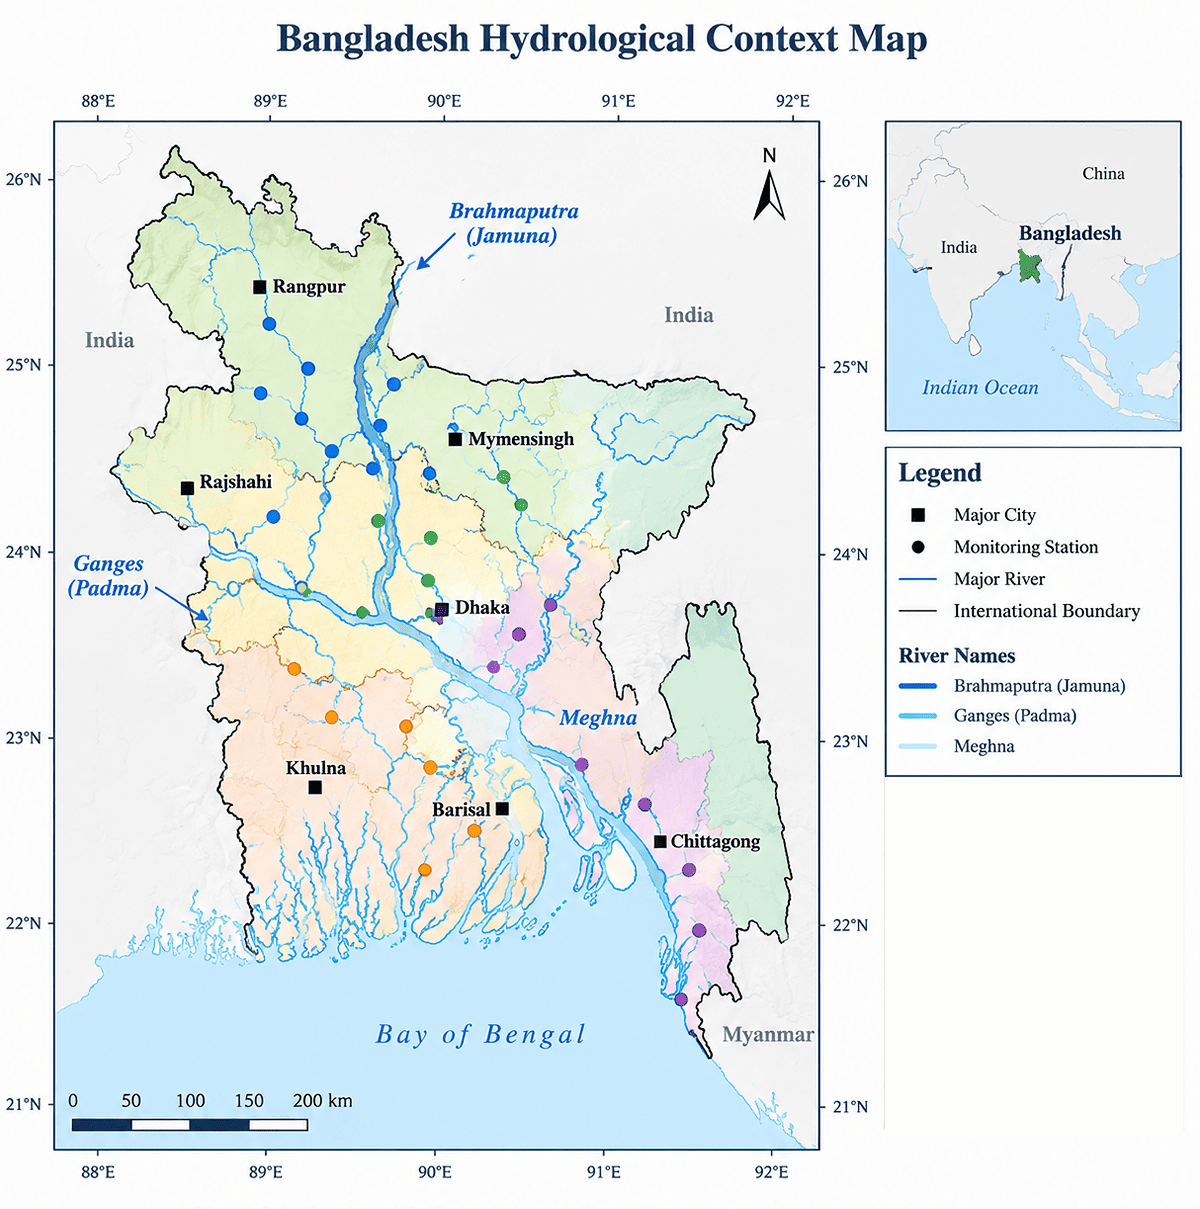
\includegraphics[width=0.85\textwidth]{figures2/fig1_1_hydro_context.png}
\caption{Bangladesh's hydrological context, showing major rivers, cities, and the study's monitoring stations.}
\label{fig:hydro-context}
\end{figure}

Figure~\ref{fig:hydro-context} gives a sense of the terrain this thesis is actually about, before the next section gets into why that terrain behaves so differently from place to place.

That risk is not distributed evenly. Rainfall, upstream discharge, the way the river network interacts with itself, and local drainage all vary from place to place, and this shows up as real differences in water-level behaviour across the country. A model built for one location will not necessarily transfer cleanly to another. This is, in effect, the starting point for the present thesis: any forecasting approach worth building for Bangladesh has to take that spatial variability seriously rather than treat it as noise.

\section{Flooding and Water-Logging in Bangladesh}

Part of what makes Bangladesh's flood problem so hard to get ahead of is that so much of it isn't generated inside the country at all. Bangladesh sits at the bottom of the Ganges--Brahmaputra--Meghna basin, and by most hydrological accounts, only a fraction of the water moving through its rivers falls as rain within its own borders --- the rest arrives from catchments upstream, across the border in India, Nepal, Bhutan, and China. In practical terms, that means a meaningful share of what shows up in a Bangladeshi river next week was already set in motion somewhere else, days earlier, by weather nobody here experienced.

The country's flood history makes this feel less abstract. In 1988, roughly 82,000 square kilometres went under water --- close to 60\% of Bangladesh --- in what's still considered a once-in-50-to-100-year event \cite{Banglapedia2023Flood}. Ten years later, 1998 went further still: more than two-thirds of the country stayed flooded, and the death toll passed 2,300 \cite{Banglapedia2023Flood,AbdullahAlam2024}. And it hasn't stopped there --- Bangladesh has seen significant flood events recur in 2004, 2007, most years between 2009 and 2014, and again in 2020, each serious enough to damage crops, roads, and household income nationally; in 2017 specifically, families in the worst-hit areas saw their annual income fall by more than a fifth \cite{AbdullahAlam2024}. None of this is distant history. It's closer to a pattern that keeps repeating, which is really the point --- this isn't a once-in-a-generation disaster this thesis is trying to help with, it's an ordinary, recurring part of life in the floodplain, and that's exactly why even a small improvement in forecast lead time or accuracy ends up mattering to a lot of people, a lot of the time.

Where the water actually causes trouble looks different depending on where you are. In rural floodplain areas, water-logging tends to follow the river fairly directly; in Bangladesh's fast-growing cities, weak drainage often turns the same rise in water level into something considerably worse. This isn't just intuition --- studies on Bangladesh back it up, showing that even neighbouring monitoring stations on the same river can behave quite differently from each other, let alone stations spread across the whole country \cite{Islam2026a,Islam2026b}. That makes sense once you think about what each part of the river is actually responding to. Upstream stations mostly react to discharge and rainfall coming down from further up the catchment. Further down, and especially around the cities, stations are shaped by a messier mix --- river flow, local rainfall, poor drainage, sometimes tidal pull as well. So there's no real basis for assuming flooding looks or behaves the same way at every station; it plainly doesn't.

None of this has gone unnoticed by researchers, to be fair. Ruma et al.\ forecast water levels across a wide network of Bangladeshi river stations using an optimized LSTM \cite{Ruma2023}. Others came at it from the meteorological side, pairing climatic variables with machine learning or deep learning to predict flooding \cite{Rakin2023,Rajab2023}, while more recent work has zeroed in on river discharge and broader hydrological modelling specifically in the Old Brahmaputra basin \cite{Islam2026a,Islam2026b}. Put together, these studies build a pretty convincing case that data-driven forecasting can work here --- but they also keep landing, sometimes explicitly, on the same conclusion: individual stations have their own character, and averaging that away loses something real.

\section{Importance of Water-Level Forecasting}

Given all this, forecasting that is reliable, timely, and sensitive to where a station actually sits in the river network is important for flood preparedness, early warning, and reducing disaster risk more generally. Different lead times are useful for different kinds of decisions: a forecast a few hours ahead supports an immediate response, while a forecast weeks ahead is more useful for planning.

The lead time itself matters a great deal, because the further out a forecast reaches, the harder it generally becomes to get right. Even so, machine-learning and deep-learning models have shown real potential for multi-step forecasting that extends to several days or weeks ahead \cite{Islam2026a,Ruma2023}. Encoder--Decoder architectures have specifically been explored for multi-step-ahead flood forecasting and offer a natural way of producing a whole sequence of future values rather than a single prediction at a time \cite{Kao2020,Cui2022}, though it is worth noting that both of these studies were evaluated at horizons of hours rather than days --- a distinction this thesis returns to in Chapter 2.

A framework that can forecast across several horizons at once, from the near-term to the longer-term, therefore offers a more complete picture of what is likely to happen than one built around a single lead time alone.

\section{Problem Statement}

Most of the water-level and flood-forecasting work done in Bangladesh so far leans on one particular type of data, or a fairly narrow combination of variables. Ruma et al. worked from water-level records alone \cite{Ruma2023}; more recent work on river discharge has largely done the same with discharge \cite{Islam2026a}; and a separate strand of research has approached flood prediction almost entirely through climatic and meteorological information \cite{Rakin2023,Rajab2023,HemelSakib2024}. Each of these lines of work is useful in its own right, but none of them really grapples with what happens when discharge, water level, and weather variables are brought together across a large and hydrologically varied network of stations.

There is a second, related issue: where the data actually comes from. Stations in different parts of a river network can behave quite differently from one another statistically, and a single model trained on pooled data from all of them may end up representing none of them particularly well. Bangladeshi hydrological studies have already applied machine-learning and deep-learning models across multiple sites, but almost always under the assumption that the data can first be brought together in one place \cite{Islam2026a,Islam2026b,Ruma2023}.

Federated learning offers a different way of thinking about this. Rather than pooling data, distributed clients train collaboratively while keeping their raw data where it is. McMahan et al.'s Federated Averaging (FedAvg) algorithm was the first to show, convincingly, how model updates from many separate clients could be combined into a single shared model without ever collecting their underlying data centrally \cite{McMahan2017}. The catch is that this works best when client data are reasonably similar to one another; when they are not --- when they are, in the technical sense, non-independent and identically distributed, or non-IID --- standard federated learning can struggle \cite{Zhu2021,Chen2025}. That kind of heterogeneity is exactly what one would expect across stations that sit in different parts of a river system.

Clustered Federated Learning (CFL) is one response to that problem: rather than forcing every client into a single shared model, clients that look similar to one another are grouped together and trained as a cluster. Work in this area has shown that this kind of grouping can produce more specialized, better-performing models than either a single global model or fully isolated local ones \cite{Ghosh2021,Harshvardhan2022,BenAli2026}. What is missing is any application of this idea to a real, multi-station, multi-horizon water-level forecasting problem in Bangladesh.

There is also a more practical concern. A forecast is only as useful as the trust placed in it, and that trust is harder to build when a model cannot explain why it predicted what it predicted. Explainable AI methods address this gap directly. SHAP, in particular, has become a widely used and theoretically well-grounded way of attributing a model's prediction to its individual inputs \cite{Lundberg2017}, and it has already been applied usefully in flood and water-level prediction \cite{Huang2024,Khorrami2025}.

Put together, the central problem this thesis addresses is how to forecast water levels accurately, across multiple horizons, for a network of Bangladeshi monitoring stations that are hydrologically quite different from one another, without needing to centralize their raw data, and while still being able to explain what is driving the model's predictions.

\section{Research Motivation}

Three strands of existing work, taken together, motivate this study.

The first concerns architecture. Deep sequence models, and LSTM in particular, have repeatedly proven effective for hydrological time series, including multi-step-ahead prediction \cite{Ruma2023,Kao2020,Cui2022}. Encoder--Decoder LSTM designs are especially well suited to this, since they naturally produce a sequence of future values rather than a single one \cite{Kao2020,Cui2022}, and more recent Seq2Seq and residual-LSTM variants confirm that this general approach remains relevant \cite{Lim2025,Yuan2023}. This is the main reason an Encoder--Decoder LSTM is chosen as the core forecasting architecture here.

The second strand is about how training happens rather than what is being trained. Federated learning makes it possible to train collaboratively while leaving raw observations where they are \cite{McMahan2017}, but non-IID data among clients is a genuine obstacle to doing this well \cite{Zhu2021,Chen2025}. Clustering clients before training, rather than after something has already gone wrong, is one practical way around this \cite{Ghosh2021,Harshvardhan2022,BenAli2026}, and there is at least one early example of federated learning being applied to hydrological forecasting specifically \cite{Amanzholova2026}, which suggests the idea is workable, even if not yet explored at any scale.

The third strand concerns trust and interpretability. As machine-learning models get folded into decisions that matter --- flood warnings among them --- being able to say why a model predicted what it did becomes as important as the prediction itself. SHAP provides a principled way of doing this \cite{Lundberg2017}, and its use in flood-related modelling has already shown that it can surface genuinely useful relationships between hydrometeorological inputs and model outputs \cite{Huang2024,Khorrami2025,Parasar2025}.

None of these three strands, on their own, is new. What has not been done is bringing them together --- multivariate hydrometeorological inputs, an Encoder--Decoder architecture, cluster-aware federated training, forecasting across multiple horizons, and interpretability --- into a single framework built for the Bangladeshi context.

\section{Research Gap}

Progress has clearly been made on each front separately: Bangladesh-specific forecasting, multi-step deep learning, federated learning, clustered federated learning, and explainable hydrological modelling all have a reasonably developed literature behind them. What they do not have, so far, is much overlap.

Bangladesh-focused studies have shown that machine learning and deep learning can forecast water level, discharge, and flood occurrence reasonably well \cite{Islam2026a,Islam2026b,Ruma2023,Rakin2023,Rajab2023,HemelSakib2024}. Separately, work on multi-step forecasting has established that Encoder--Decoder and Seq2Seq architectures are a sound way of generating forecasts across several future time steps \cite{Kao2020,Cui2022,Lim2025,Yuan2023}. Federated learning research has tackled decentralized training and the non-IID problem in general terms \cite{McMahan2017,Zhu2021,Chen2025}, and clustered federated learning has offered a specific mechanism --- grouping similar clients --- for handling that heterogeneity \cite{Ghosh2021,Harshvardhan2022,BenAli2026}. And SHAP-based explainability has already found its way into flood and hydrological modelling \cite{Lundberg2017,Huang2024,Khorrami2025}.

But no study identified in this review brings these threads together: multi-horizon water-level forecasting, across a large and multivariate network of Bangladeshi stations, using a cluster-aware federated architecture, with SHAP-based interpretation, and checked against an external reference such as the Flood Forecasting and Warning Centre (FFWC).

That is the gap this thesis sets out to close, with a Clustered Federated Learning framework built around an Encoder--Decoder LSTM (CFL-EDLSTM) for multi-horizon water-level forecasting in Bangladesh.

\section{Aim of the Study}

The aim of this study is to design, build, and evaluate a Clustered Federated Learning framework based on an Encoder--Decoder LSTM (CFL-EDLSTM), for privacy-preserving, multi-horizon, and interpretable water-level forecasting across 25 hydrologically diverse monitoring stations along the Brahmaputra River system in Bangladesh.

Alongside the forecasting framework itself, the study also demonstrates how these outputs might actually be presented to someone using them, through a web-based visualization platform. The platform gives station-level forecast information and lets a user compare CFL-EDLSTM's predictions against water-level information published by the Flood Forecasting and Warning Centre (FFWC), used here as an external point of comparison rather than as ground truth.

\section{Research Objectives}

The objectives of this study are:

\begin{enumerate}
    \item To develop a clustering strategy that groups 25 hydrologically diverse Bangladeshi monitoring stations within the Brahmaputra River system into four meaningful clusters: Upstream, Middle, Downstream, and Urban.

    \item To develop an Encoder--Decoder LSTM (EDLSTM) architecture capable of multivariate, multi-horizon water-level forecasting across seven lead times, ranging from 3 hours to 15 days.

    \item To integrate the EDLSTM architecture within a Clustered Federated Learning (CFL) framework using Federated Averaging (FedAvg) for cluster-specific parameter aggregation without centralizing raw station-level data.

    \item To benchmark the proposed CFL-EDLSTM framework against four baseline architectures --- Vanilla LSTM, GRU, XGBoost, and TCN --- across different station clusters and forecast horizons.

    \item To apply SHAP-based interpretability to the trained models in order to identify and rank the hydrometeorological variables contributing to model predictions.

    \item To develop a web-based visualization platform that presents CFL-EDLSTM forecasts and compares them against water-level information published by the Flood Forecasting and Warning Centre (FFWC) as an external reference.
\end{enumerate}

\section{Research Questions}

This study is guided by the following questions:

\begin{enumerate}
    \item How can 25 hydrologically diverse monitoring stations within the Brahmaputra River system in Bangladesh be grouped into clusters that are meaningful for federated training?

    \item How effectively can an Encoder--Decoder LSTM architecture forecast water levels across horizons ranging from short-term (3 hours) to long-term (15 days)?

    \item How well does the proposed Clustered Federated Learning approach handle heterogeneity among the four station clusters while keeping station-level data private?

    \item How does the proposed CFL-EDLSTM framework perform relative to Vanilla LSTM, GRU, XGBoost, and TCN baselines across different clusters and lead times?

    \item Which input variables --- water level, discharge, rainfall, temperature, or evaporation --- contribute most to model predictions according to SHAP, and do those contributions make hydrological sense?

    \item How closely do CFL-EDLSTM's forecasts, as shown through the web-based visualization platform, align with water-level information published by FFWC, used here as an external point of comparison rather than as ground truth?
\end{enumerate}

\section{Scope of the Study}

This study is built around 25 selected monitoring stations within the Brahmaputra River system in Bangladesh, grouped into four clusters --- Upstream, Middle, Downstream, and Urban --- based on their hydrological characteristics and where they sit within the river network.

Five variables are used: water level, discharge, rainfall, temperature, and evaporation, with water level as the target. Forecasts are generated across seven lead times: 3 hours, 6 hours, 12 hours, 1 day, 3 days, 7 days, and 15 days.

CFL-EDLSTM is compared against four baseline architectures --- Vanilla LSTM, GRU, XGBoost, and TCN --- reflecting the broader set of modelling approaches identified in recent flood-prediction literature \cite{Aghenda2025}, and interpreted using SHAP \cite{Lundberg2017,Huang2024}.

What this study does not attempt is real-time operational deployment, a mobile application, or forecasting of anything beyond water level. The web-based visualization interface is built to demonstrate and validate the framework, not to serve as an operational early-warning system in its own right.

\section{Contributions of the Study}

This thesis makes the following contributions:

\begin{enumerate}
    \item A clustering strategy that groups 25 monitoring stations within the Brahmaputra River system into four meaningful federated client groups: Upstream, Middle, Downstream, and Urban.

    \item A Clustered Federated Learning framework based on an Encoder--Decoder LSTM (CFL-EDLSTM), for privacy-preserving, multivariate, multi-horizon water-level forecasting across heterogeneous monitoring stations.

    \item A comparative evaluation of CFL-EDLSTM against four established baseline architectures across multiple station clusters and seven forecast horizons.

    \item A SHAP-based interpretability analysis identifying which hydrometeorological variables matter most, and where, across the different station clusters.

    \item A web-based visualization and comparison platform that presents CFL-EDLSTM forecasts alongside FFWC water-level information, showing how the framework's results might practically be used.
\end{enumerate}

\section{Overview of the Proposed Framework}

At a high level, CFL-EDLSTM combines a sequence-to-sequence Encoder--Decoder LSTM \cite{Kao2020,Cui2022} with a Clustered Federated Learning training procedure. The federated part of this borrows directly from McMahan et al.'s original idea: model updates travel from distributed clients to a central point of aggregation, but the raw data behind those updates never does \cite{McMahan2017}.

In this framework, the 25 monitoring stations are first grouped into four clusters based on their hydrological characteristics and position within the river network. Each station then acts as a local client within its cluster, training the EDLSTM model on its own multivariate data. Rather than being sent anywhere, that data stays local; only the resulting model parameters are shared, and Federated Averaging (FedAvg) is used to combine them into a single model per cluster \cite{McMahan2017}.

This is a deliberate departure from a conventional federated setup, where all clients would ultimately contribute to one shared global model. Here, each cluster keeps its own model. The reasoning follows directly from the literature reviewed above: non-IID data across clients can genuinely hurt standard federated learning \cite{Zhu2021,Chen2025}, whereas clustering clients with similar characteristics tends to produce better, more specialized models \cite{Ghosh2021,Harshvardhan2022,BenAli2026}.

Once trained, the four cluster models generate water-level forecasts across all seven horizons. SHAP is then applied to interpret those forecasts and see which variables are actually driving them \cite{Lundberg2017,Huang2024,Khorrami2025}. Finally, everything is made accessible through an interactive web-based map, with a separate section for comparing the model's output against FFWC's published water-level information.

The full implementation and experimental design behind this framework are described in Chapter 3.

\section{Organization of the Thesis}

The rest of this thesis is organized into four chapters.

\textbf{Chapter 2} reviews the literature underpinning this study --- Bangladesh-specific flood and water-level forecasting, hydrological and meteorological time-series modelling, machine learning and deep learning, Encoder--Decoder LSTM architectures, multi-horizon forecasting, federated learning, clustered federated learning, and explainable AI --- and closes with a critical synthesis that identifies the specific gap this thesis addresses.

\textbf{Chapter 3} sets out the methodology: the study area, monitoring stations, data sources, input and target variables, preprocessing, the station-clustering strategy, the forecasting setup, the proposed CFL-EDLSTM architecture and its federated aggregation procedure, the baseline models, the multi-horizon evaluation design, the performance metrics, the SHAP analysis, and the web-based visualization platform.

\textbf{Chapter 4}, once experiments have been run, will present and discuss the results --- the clustering outcomes, CFL-EDLSTM's overall performance, its comparison against the baselines, its performance across different horizons and clusters, the SHAP findings, station-level visualizations, and the comparison against FFWC.

\textbf{Chapter 5} will close the thesis with a summary of what was found, how well the objectives were met, the study's contributions and limitations, and directions for future work.



\chapter{Literature Review}
\label{Ch_Chapter2}

\section{Introduction}

This chapter works through the literature that sits behind the proposed Clustered Federated Learning Encoder--Decoder LSTM (CFL-EDLSTM) framework. It starts broad, with flood and water-level forecasting as a field and the kind of hydrological and meteorological data typically used to do it, then narrows step by step: traditional statistical methods, machine learning, deep learning, and within deep learning, the specific architectures --- Vanilla LSTM, GRU, XGBoost, and TCN --- that matter for this thesis. From there it moves into multi-horizon forecasting and station heterogeneity, which is really where the argument for federated and clustered learning begins, before covering explainable AI and, more briefly, visualization. The chapter closes with a critical comparison of everything covered and a clear statement of the gap this thesis is trying to fill.

\begin{figure}[h]
\centering
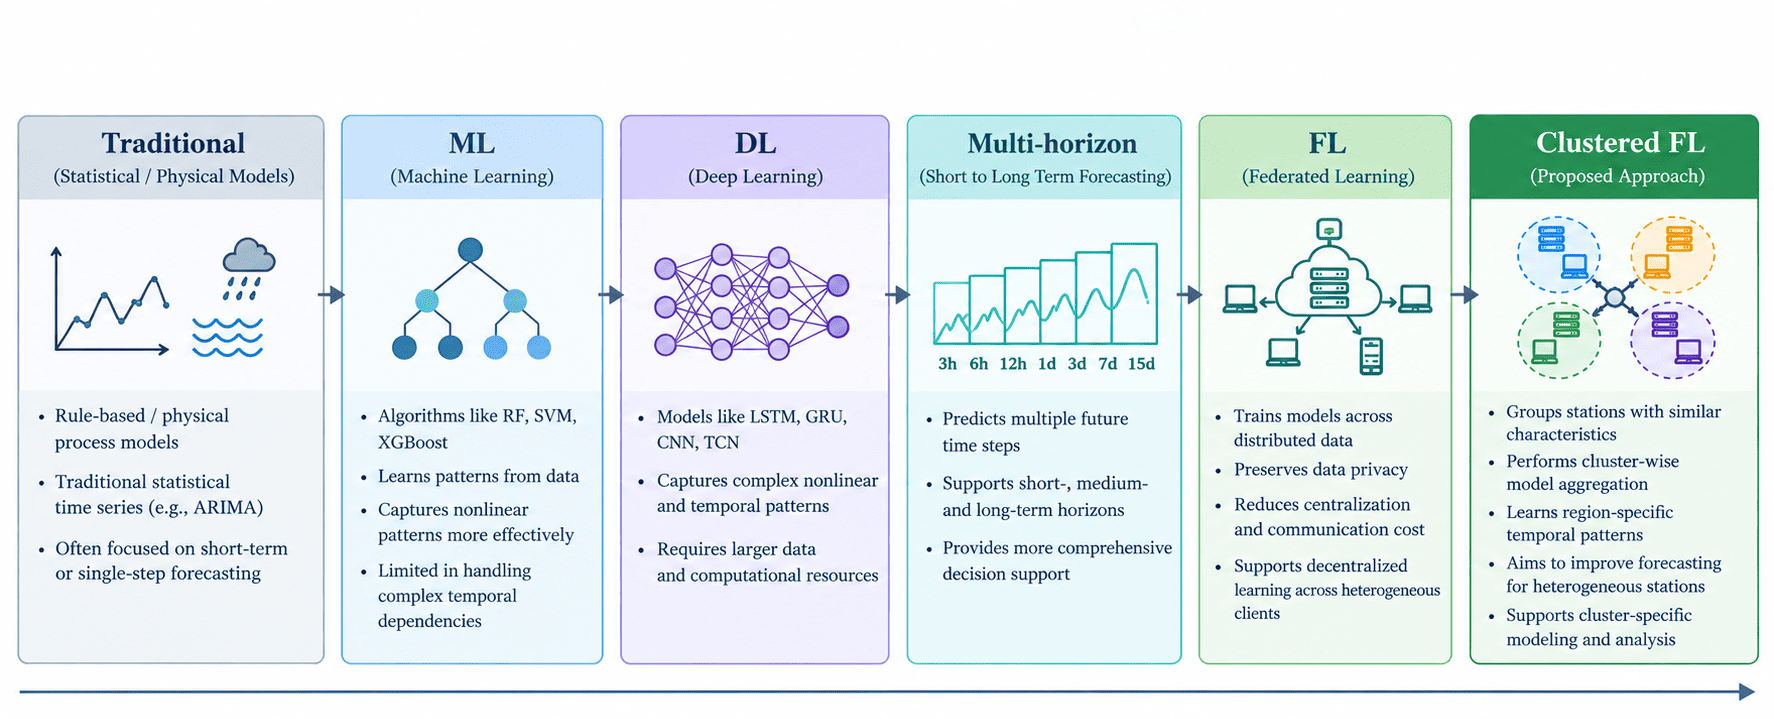
\includegraphics[width=\textwidth]{figures2/fig2_1_lit_evolution.png}
\caption{Conceptual evolution of water-level forecasting approaches, from traditional methods to the proposed CFL framework.}
\label{fig:lit-evolution}
\end{figure}

Figure~\ref{fig:lit-evolution} lays that progression out visually before the chapter walks through it section by section.

\section{Flood and Water-Level Forecasting}

Flood and water-level forecasting, in its broadest sense, means predicting future river or reservoir conditions --- water level, discharge, or the occurrence of a flood --- from historical hydrological and meteorological records, with early warning and risk management as the end goal. A systematic review covering 363 flood-prediction studies published between 2018 and 2025 found that data-driven methods, machine learning and deep learning in particular, now dominate the field across global and South Asian contexts, and, interestingly, that no single model architecture wins consistently across every study \cite{Aghenda2025}. A related review of deep-learning applications in flood forecasting reached much the same conclusion, noting that architectures ranging from feed-forward networks to convolutional and recurrent networks, along with various hybrids, have all been applied to river-flow, water-level, and flood-hazard problems, while data quality, interpretability, and computational cost remain recurring sticking points \cite{Kumar2023}.

Bangladesh has its own, fairly substantial body of work in this space, drawing mostly on records from the Bangladesh Water Development Board (BWDB) and the Bangladesh Meteorological Department (BMD), and combining hydrological and meteorological data in varying ways \cite{Islam2026a,Islam2026b,Ruma2023,Rakin2023,Rajab2023,HemelSakib2024}. Between them, these studies show that data-driven forecasting is genuinely feasible in the Bangladeshi context. What they use as input, though, differs quite a bit from one study to the next, which is where the next section picks up.

\section{Hydrological and Meteorological Data}

How much data a study actually uses, and of what kind, turns out to be one of the more telling differences across this literature --- and it is a large part of the motivation for this thesis. Some studies work from a single variable. Ruma et al. forecast water level using nothing but historical water-level records across a network of Bangladeshi river stations \cite{Ruma2023}; Islam et al., working the discharge side of things at two stations in the Old Brahmaputra basin, do much the same with discharge alone, and are upfront that leaving out meteorological variables such as precipitation is a real limitation of their study \cite{Islam2026a}.

Others combine variables. A separate study by Islam et al. brings together daily water level with rainfall and temperature at the Islampur and Sarishabari stations, using 1--5 day lag features to capture how the river responds to monsoon rainfall with a delay \cite{Islam2026b}. Cui et al. combine discharge and inflow with areal rainfall and evaporation, both computed with the Thiessen polygon method from several gauge stations \cite{Cui2022}. Rajab et al., forecasting rainfall itself as the target, use a correlation-based feature-selection step that trims an initial 18 meteorological features down to 16 \cite{Rajab2023}.

A third group skips hydrological data entirely and works only from meteorology. Rakin et al. and Hemel and Sakib both build their flood-occurrence classifiers purely from BMD weather records --- rainfall, temperature, and related variables --- with no discharge or water-level measurements involved at all \cite{Rakin2023,HemelSakib2024}. Put these three groups side by side and a fairly obvious gap appears: no Bangladeshi study reviewed here brings discharge, water level, rainfall, temperature, and evaporation together in one framework. Section 2.15 returns to this.

\section{Traditional Statistical Approaches}

Before machine learning took over, flood forecasting relied mostly on physically based hydrological models and classical statistical regression. Almost none of the literature collected for this thesis is purely statistical in that older sense --- it is nearly all machine-learning or deep-learning work --- but a couple of studies do include regression methods as part of their comparisons, and these are worth looking at for what they say about how far classical methods still get you. Rajab et al. tested Multiple Linear Regression and Polynomial Regression alongside a long list of machine-learning and deep-learning models for BMD rainfall forecasting, and found Random Forest ($R^2 = 0.768$ on the test set) and Polynomial Regression ($R^2 = 0.764$) among the stronger performers, not far off the reported LSTM results \cite{Rajab2023}. Islam et al. similarly kept Linear Regression in the mix alongside Random Forest, XGBoost, LightGBM, and LSTM when forecasting daily water level in the Old Brahmaputra basin \cite{Islam2026b}.

What this suggests, unsurprisingly, is that regression still has a place as a simple, interpretable baseline, but it tends to fall short of tree-based ensembles and deep learning once the relationships being modelled get properly nonlinear and time-dependent, which is exactly the case for hydrological data. That is the direction the rest of this chapter follows.

\section{Machine Learning-Based Forecasting}

Beyond plain regression, ensemble and kernel-based methods have been applied fairly widely to flood-related forecasting. Rakin et al. put ten machine-learning and deep-learning classifiers up against each other for Bangladesh flood occurrence, using 65 years of BMD weather data across 32 districts; LightGBM came out on top at 97.76\% accuracy, with Random Forest close behind at 97.71\% \cite{Rakin2023}. Hemel and Sakib ran a smaller comparison --- Logistic Regression, Random Forest, Gradient Boosting, XGBoost, and LSTM --- and found Gradient Boosting the strongest, at 95.38\% \cite{HemelSakib2024}.

For continuous targets, the picture is similar. Islam et al. compared Random Forest, LightGBM, and Support Vector Regression against LSTM and BiLSTM for discharge forecasting in the Old Brahmaputra basin, and while LSTM and BiLSTM ultimately came out ahead on composite performance, the tree-based and kernel-based models were not far off \cite{Islam2026a}. Hossain et al. ran a comparable comparison --- Linear Regression, Random Forest, XGBoost, MLP, LightGBM, and Polynomial Regression --- for monthly extreme water-level prediction at Islampur, using 34 years of records \cite{Hossain2025}. Perhaps the clearest single result here comes from Hameed et al., who found XGBoost beating both LSTM and Random Forest outright for monthly runoff forecasting in a glacierized catchment ($R^2 = 0.904$, NSE $= 0.797$) \cite{Hameed2025} --- a useful reminder that gradient-boosted trees are not just a fallback option when deep learning is unavailable, but a genuinely competitive method in their own right.

\section{Deep Learning for Water-Level Forecasting}

Even so, deep learning is where most of the recent activity in hydrological forecasting has gone. Aghenda et al.'s systematic review found LSTM to be the single most common architecture across the 363 studies they looked at, making up 21\% of all implementations \cite{Aghenda2025}. Kumar et al. reach a broadly similar conclusion, pointing to LSTM and GRU as particularly good at capturing temporal dependencies, with convolutional and hybrid variants such as ConvLSTM additionally able to pick up spatial patterns \cite{Kumar2023}. Waqas and Humphries explain why this works: ordinary RNNs suffer from vanishing and exploding gradients that make it hard for them to learn long-range dependencies, and LSTM's gating mechanism is specifically built to get around that \cite{Waqas2024}. The four subsections that follow look more closely at LSTM, GRU, Encoder--Decoder LSTM, and TCN in turn.

\subsection{LSTM}

Ruma et al. give a direct example of LSTM applied to Bangladesh: combined with particle swarm optimization (PSO-LSTM), their model forecasts water level across river stations on the Ganges, Brahmaputra, and Meghna, reaching an NSE of roughly 0.957 at a 15-day horizon \cite{Ruma2023}. Waqas and Humphries' review covers a much wider set of LSTM variants used in hydrology --- Bidirectional LSTM, Stacked LSTM, attention-based LSTM, and hybrids like LSTM-CNN, wavelet-LSTM, and LSTM-Transformer --- and conclude that LSTM architectures generally beat plain RNNs and GRUs on hydrological prediction, though hyperparameter sensitivity and weak generalization across different hydrological settings remain genuine problems \cite{Waqas2024}. This fits with Aghenda et al.'s finding that LSTM leads the field overall \cite{Aghenda2025}. What none of these studies do, though, is use LSTM as part of a sequence-to-sequence, multi-cluster, or federated setup --- each treats it as a single-station, single-step (or fixed-horizon) model, which is exactly the space the Encoder--Decoder and federated components of this thesis are meant to fill.

\subsection{GRU}

GRU trades some of LSTM's complexity for a simpler gating structure while still handling temporal dependencies reasonably well. Ni et al. paired GRU with TCN in a hybrid architecture that also used kernel density estimation for error bounds, and reported a 13\% RMSE reduction over standalone LSTM, GRU, and TCN \cite{Ni2024}. Li et al. included GRU as one of several baselines --- alongside RNN, LSTM, TCN, and Attention-TCN --- for streamflow forecasting in semi-arid basins, using around 20 years of daily hydrometeorological data \cite{Li2024}. Waqas and Humphries also note that GRU shows up combined with LSTM in hybrid forms elsewhere in the literature \cite{Waqas2024}. On the whole, GRU comes across as a reasonable, lighter alternative to LSTM rather than a clear improvement on it; this thesis treats it accordingly, as a baseline to compare CFL-EDLSTM against (Section 3.13) rather than as a candidate for the core architecture.

\subsection{Encoder--Decoder LSTM}

The Encoder--Decoder LSTM turns multi-step forecasting into a sequence-to-sequence problem: an encoder compresses a window of past observations into a fixed representation, and a decoder unrolls that into a sequence of future predictions. Kao et al. were among the first to apply this specifically to flood forecasting, working with hourly data from 23 typhoon events in Taiwan's Shihmen Reservoir catchment and rainfall from 10 gauge stations, forecasting reservoir inflow from one to six hours ahead. Their LSTM-ED beat a feed-forward encoder--decoder benchmark by about 3\% RMSE at the one-hour mark, and by roughly 38\% by the six-hour mark ($R^2$ around 0.98 and 0.88 respectively) --- a gap that widens with the horizon, which is itself a useful finding: the benefit of the encoder--decoder design over a simpler benchmark grows the further out you try to forecast \cite{Kao2020}.

Cui et al. took this a step further with an Encoder--Decoder that feeds an exogenous, process-model-derived forecast into the decoder (LSTM-EDE), tested across 3-, 6-, 9-, and 12-hour horizons in two Chinese basins. It came out ahead of the alternatives they compared it against, and, notably, degraded the least as the horizon lengthened, with NSE of 0.81 (Lushui) and 0.93 (Jianxi) at 12 hours \cite{Cui2022}. More recently, Lim et al. built a Seq2Seq LSTM surrogate model for real-time, multi-step flood forecasting in a coastal-urban setting and found it outperformed a standard LSTM \cite{Lim2025}, and Yuan et al. proposed a Time Residual LSTM aimed directly at fixing the degradation problem observed in Kao et al.'s original LSTM-ED baseline \cite{Kao2020,Yuan2023}. Across all four studies, the pattern holds: encoder--decoder designs consistently hold up better at longer horizons than the alternatives they are compared against. What none of them do is push past a 12-hour horizon, or train across more than one site at a time --- both of which this thesis attempts, extending the same architectural idea out to 15 days and across 26 stations grouped into four clusters.

\subsection{TCN}

The Temporal Convolutional Network takes a different route entirely, using dilated causal convolutions instead of recurrence. Lin et al. compared TCN against ANN, LSTM, and EIESM for multi-lead-time flood forecasting and found it held its own against LSTM on NSE, RMSE, and bias, though it lost ground at longer lead times \cite{Lin2021}. Li et al.'s attention-augmented version, Attention-TCN, did better still, cutting MAE by 6.9--25\% relative to a standard LSTM on heterogeneous semi-arid streamflow data \cite{Li2024}, and Ni et al.'s GRU-TCN hybrid, mentioned above, outperformed a standalone TCN as well as standalone LSTM and GRU \cite{Ni2024}. At the far end of the horizon range, Li et al. reported a hybrid combining Empirical Mode Decomposition with TCN and GRU that reached very high accuracy ($R^2 = 0.9922$, MAPE $= 3.25\%$) for 15-day streamflow forecasting, though at considerably more architectural complexity than a plain TCN \cite{Li2025}. TCN, then, is a credible non-recurrent alternative to LSTM, and it earns its place in this thesis as one of the four baseline models (Section 3.13), even though --- like the studies above --- it has not previously been tested in a multi-station or federated setting.

\section{Tree-Based Models}

Gradient-boosted decision trees sit apart from both the classical regression methods discussed in Section 2.4 and the neural architectures above, and, as already noted in Section 2.5, hold up surprisingly well in hydrological forecasting.

\subsection{XGBoost}

XGBoost in particular shows up repeatedly across this literature, both as a standalone model and as a comparison baseline. Hameed et al.'s finding that it outperforms LSTM and Random Forest for monthly runoff forecasting ($R^2 = 0.904$, NSE $= 0.797$) is probably the strongest single piece of evidence for this \cite{Hameed2025}. Within Bangladesh specifically, Hossain et al. include it among six models compared for monthly extreme water-level prediction at Islampur \cite{Hossain2025}, and Islam et al. include it in their daily water-level comparison at Islampur and Sarishabari \cite{Islam2026b}. Rakin et al. and Hemel and Sakib both use it as one of several classifiers for Bangladesh flood occurrence, with Hemel and Sakib reporting 94.47\% accuracy for it specifically \cite{Rakin2023,HemelSakib2024}. Every one of these evaluations, though, is confined to a single station or a single-site classification problem. This thesis instead runs XGBoost consistently as a baseline across all four clusters and all seven horizons (Section 3.13) --- a scale of comparison none of the studies above attempt.

\section{Multi-Horizon Forecasting}

Forecast accuracy tends to drop as the horizon lengthens, and several studies document this directly rather than just assuming it. Kao et al.'s LSTM-ED advantage over a feed-forward benchmark widened from 3\% at one hour to 38\% at six hours \cite{Kao2020}; Cui et al. found their exogenous-input design degraded the least, of the architectures they tested, up to 12 hours \cite{Cui2022}; and Yuan et al. built a Time Residual LSTM specifically to address the degradation seen in Kao et al.'s baseline at longer horizons \cite{Kao2020,Yuan2023}.

At the longer end, the evidence gets thinner but still points in a useful direction. Ruma et al. showed that 15-day water-level forecasting is achievable in Bangladesh (NSE $\approx 0.957$) \cite{Ruma2023}, and Islam et al. tested discharge forecasting across six horizons out to 30 days, finding LSTM strongest specifically at the 15- and 30-day marks \cite{Islam2026a}. Li et al.'s hybrid decomposition model reached $R^2 = 0.9922$ at a 15-day streamflow horizon \cite{Li2025}, which is a useful benchmark to keep in mind for what "good" might look like at the longest horizon considered here. None of these studies, though, evaluates one architecture across a range as wide as 3 hours to 15 days, which is precisely the design adopted in this thesis.

\section{Heterogeneity in Monitoring Stations}

There is also fairly direct evidence that station behaviour differs, sometimes considerably, even within a single river system. Islam et al. trained a discharge model at Mymensingh and tested it at the nearby Islampur station without retraining; performance held up reasonably well overall, but it varied by location and by horizon \cite{Islam2026a}. A related study by Islam et al. did much the same between Islampur and Sarishabari, again finding that how well a model transferred depended on the input scenario and the specific target station \cite{Islam2026b}. What this really shows is that even geographically close stations within the same sub-basin are different enough, statistically, for model performance to shift noticeably between them --- which is more or less the non-IID problem that federated learning research describes in general terms \cite{Zhu2021,Chen2025}, covered next.

\section{Federated Learning}

Federated learning lets distributed parties train a model together without any of them having to hand over their raw data --- a natural fit for a setting where hydrological and meteorological records are held separately by different stations or offices, as they typically are in Bangladesh.

\subsection{Conventional FL}

McMahan et al.'s Federated Averaging (FedAvg) algorithm is where this line of work begins. Clients run several rounds of local training before a central server averages their model parameters into a shared model; tested on MNIST, CIFAR-10, and language-modelling tasks, this cut the number of communication rounds needed to reach a target accuracy by roughly one to two orders of magnitude compared with plain federated SGD \cite{McMahan2017}. That basic idea --- train locally, share only the parameters, never the data --- is the mechanism this thesis borrows for training across monitoring stations. It is worth being clear, though, that FedAvg itself was built and tested on generic image and language benchmarks, under the assumption of a single shared model; it says nothing about hydrology, and nothing about what happens when the clients involved are genuinely dissimilar from one another, which is exactly the problem taken up in Section 2.10.3.

\subsection{FL for Time-Series}

Federated learning applied specifically to hydrological time series is still fairly rare, but there is at least one direct precedent. Amanzholova et al. built a federated LSTM for next-day discharge forecasting at two stations in the transboundary Chu--Talas basin, comparing it against centralized and local-only versions. At the more homogeneous of the two stations, the federated model came within about 1\% of the centralized one (NSE $0.948$ versus $0.956$); at the station with more divergent behaviour, it clearly outperformed both alternatives (NSE $0.903$, against $0.528$ centralized and $-4.230$ local-only) \cite{Amanzholova2026}. Chen et al. make a similar point more generally, using non-hydrological time-series benchmarks to show that standard federated learning struggles once client data become properly heterogeneous \cite{Chen2025}. Amanzholova et al.'s result is encouraging, but it covers only two stations, one variable, and a single one-day horizon, with no clustering involved; this thesis is, in effect, an attempt to see whether the same basic approach holds up at a rather larger scale --- 26 stations, five variables, seven horizons, and an explicit clustering step.

\subsection{Non-IID Data}

The practical difficulty with federated learning is that client data are rarely as similar to one another as the theory would like. Zhu et al.'s survey lays this out clearly: non-IID data across clients can cause slower convergence, degraded accuracy, and outright divergence under standard FedAvg, and they review a range of data-based and algorithmic fixes across both horizontal and vertical federated learning \cite{Zhu2021}. Chen et al. show much the same thing for time-series data specifically \cite{Chen2025}. This maps quite directly onto the station heterogeneity discussed in Section 2.9, where forecasting performance was shown to shift even between neighbouring stations on the same river \cite{Islam2026a,Islam2026b}. Neither Zhu et al. nor Chen et al. propose a hydrology-specific fix, though --- they describe the problem rather than solve it for this domain, which leaves the actual mitigation strategy, clustering clients before training, to the next section.

\section{Clustered and Federated Learning}

Clustered Federated Learning takes a fairly intuitive approach to the non-IID problem: instead of forcing every client into one shared model, group clients that look similar and train a model per group. Ghosh et al.'s Iterative Federated Clustering Algorithm (IFCA) does this by repeatedly estimating which cluster each client belongs to and updating that cluster's model accordingly, and it clearly beats both a single global model and fully local training on heterogeneous benchmarks --- 95.25\% accuracy versus 89.73\% and 80.05\% on a four-cluster Rotated MNIST setup, and 81.51\% versus 77.87\% and 33.97\% on a two-cluster Rotated CIFAR setup \cite{Ghosh2021}.

Harshvardhan et al.'s Successive Refine Federated Clustering Algorithm (SR-FCA) improves on this in one important way: it does not need to know the number of clusters in advance, unlike IFCA. It also comes out ahead of Local, Global, and IFCA baselines across several benchmarks --- 92.84\% on inverted MNIST, 91.83\% on rotated MNIST, 88.70\% on rotated CIFAR-10, and 84.93\% on FEMNIST \cite{Harshvardhan2022}. Ben Ali et al. step back from individual algorithms and organize the field into a taxonomy --- server-side clustering (based on model weights or gradients), client-side clustering (based on training loss or model selection), and metadata-based clustering (based on shared statistical descriptors) --- while pointing out that cluster-quality metrics such as the Adjusted Rand Index, Cluster Purity, and Silhouette Score exist but that choosing the right number of clusters in the first place remains an open problem \cite{BenAli2026}.

None of these three studies has anything to do with hydrology; all of them rely on image or text benchmarks with artificially constructed heterogeneity. That leaves an obvious question unanswered: what does a "cluster" even mean when the clients are river-monitoring stations rather than benchmark partitions? The CFL literature clusters clients by model similarity or by statistical metadata; this thesis instead defines its four clusters --- Upstream, Middle, Downstream, Urban --- using hydrological domain knowledge, an approach none of the algorithms above were tested against.

\section{Explainable AI}

The more accurate hydrological forecasting models have become, the more it has mattered that someone can actually explain their predictions, particularly where those predictions feed into early-warning decisions. Khorrami et al. reviewed 83 studies applying explainable AI to runoff and water-level forecasting, spanning both ante-hoc and post-hoc methods across several model types including LSTM, and their headline finding is that SHAP is, by a clear margin, the dominant post-hoc method in this space \cite{Khorrami2025}.

\subsection{SHAP}

SHAP itself, introduced by Lundberg and Lee, gives a theoretically grounded way of attributing a model's output to its individual input features. It unifies a number of earlier feature-attribution methods and proves that the resulting Shapley-value attribution is the only one satisfying three desirable properties --- local accuracy, missingness, and consistency; the original paper also shows SHAP to be more sample-efficient than LIME and Shapley sampling across several model types, including a CNN \cite{Lundberg2017}. It was never built with hydrology in mind, but being model-agnostic, it applies just as well there as anywhere else.

Huang et al. put this into practice, integrating SHAP (via a Gradient Explainer) into a coupled CNN-LSTM flood model for the Beijiang River Basin, built from rainfall and runoff data at 17 stations. Their model reached NSE $= 0.838$ at a 25-hour horizon, ahead of standalone CNN (0.737) and LSTM (0.745), and the SHAP analysis found that recent downstream runoff dominated the predictions, with rainfall contributing comparatively little \cite{Huang2024}. Hemel and Sakib applied SHAP and LIME together to a Gradient Boosting flood classifier for Bangladesh and identified rainfall as a particularly strong predictor \cite{HemelSakib2024}. Parasar et al. used SHAP on a hydroclimatic discharge model in a monsoon-dominated river system, and were able to show how the relative influence of rainfall versus antecedent discharge shifted under monsoon conditions not unlike those found in Bangladesh \cite{Parasar2025}. None of these three applications, though, sits inside a clustered or federated model, and none asks whether feature importance actually looks different from one part of a river network to another. That is exactly the question this thesis puts to SHAP in Section 3.16 --- computing it separately for each of the four clusters, rather than once for the whole network, to see whether the patterns Huang et al. and Parasar et al. found at single sites hold consistently, or not, across Upstream, Middle, Downstream, and Urban stations.

\section{Visualization and Decision-Support Systems}

This is, honestly, the thinnest part of the literature collected for this thesis. Lim et al.'s Seq2Seq LSTM surrogate model was explicitly built with real-time, operational use in mind for a coastal-urban flood context \cite{Lim2025}, which at least signals that practical, decision-relevant delivery is a recognized concern, even if it is rarely the main focus of a study. A number of the Bangladesh-focused papers gesture in this direction without quite getting there: Ruma et al. and Islam et al. both flag real-time, operationally grounded forecasting as a natural next step for their work \cite{Islam2026a,Ruma2023}, and Hemel and Sakib note that their classification-based approach does not incorporate real-time hydrological data \cite{HemelSakib2024}. This thesis addresses that gap fairly directly, by building an interactive web-based visualization interface (Chapter 3) that presents station-level forecasts and sets them alongside water-level information published by the FFWC, used here as an external point of comparison rather than as a validated ground truth.

\section{Critical Comparison of Existing Studies}

Stepping back, the literature reviewed in this chapter falls into four groups that, so far, have not had much to do with one another. Bangladesh-specific forecasting studies work with a single data modality at a time, ranging from a handful of specific hydrological stations to much larger pooled networks of stations or districts, but always in a centralized setting \cite{Islam2026a,Islam2026b,Ruma2023,Rakin2023,Rajab2023,HemelSakib2024,Hossain2025}. Deep-learning architecture research --- Encoder--Decoder LSTM, TCN, gradient-boosted trees --- establishes strong methods for multi-step forecasting, but almost entirely outside Bangladesh and always in a centralized setup \cite{Kao2020,Cui2022,Lim2025,Yuan2023,Ni2024,Kumar2023,Hameed2025,Waqas2024,Aghenda2025,Li2024,Lin2021,Li2025}. Federated and clustered federated learning research shows that FedAvg and cluster-specific training deal with client heterogeneity reasonably well, but only on generic benchmarks or, at most, a two-station hydrological case \cite{McMahan2017,Zhu2021,Chen2025,Ghosh2021,Harshvardhan2022,BenAli2026,Amanzholova2026}. And explainable-AI research has established SHAP as the go-to interpretability method for hydrological deep learning, without yet putting it inside a clustered or federated model \cite{Lundberg2017,Huang2024,Khorrami2025,Parasar2025}.

Table~\ref{tab:lit-comparison} lays this out more concretely, showing where each strand sits on data modality, scale and architecture, and its main limitation as far as this thesis is concerned.

\vspace{-0.3cm}
\begin{table}[htbp]
\centering
\caption{Critical comparison of the four reviewed research strands}
\label{tab:lit-comparison}
\small
\setlength{\tabcolsep}{4pt}
\renewcommand{\arraystretch}{1.25}

\begin{tabularx}{\textwidth}{
    >{\raggedright\arraybackslash}p{3.0cm}
    >{\raggedright\arraybackslash}X
    >{\raggedright\arraybackslash}X
    >{\raggedright\arraybackslash}X
}
\toprule
\textbf{Research Strand} &
\textbf{Data Modality} &
\textbf{Scale / Architecture} &
\textbf{Key Limitation} \\
\midrule

\textbf{Bangladesh-specific forecasting}
\cite{Islam2026a,Islam2026b,Ruma2023,Rakin2023,Rajab2023,HemelSakib2024,Hossain2025}
&
Single or limited data modality, including water level, discharge, rainfall, and meteorological variables
&
Ranges from 1--3 specific stations to large pooled networks (20+ stations or districts), but always trained as a single centralized model
&
No multivariate (hydrological + meteorological) integration and no cluster-specific or federated modeling, regardless of network size
\\[0.8em]

\textbf{Deep-learning architectures}
\cite{Kao2020,Cui2022,Lim2025,Yuan2023,Ni2024,Li2024,Lin2021,Li2025}
&
Hydrological and hydro-meteorological time-series data, mainly from non-Bangladesh studies
&
Mostly centralized forecasting at individual sites or datasets using LSTM, GRU, Encoder--Decoder LSTM, TCN, and related architectures
&
Limited evaluation in distributed or federated multi-station hydrological forecasting
\\[0.8em]

\textbf{Federated / Clustered Federated Learning}
\cite{McMahan2017,Zhu2021,Chen2025,Ghosh2021,Harshvardhan2022,BenAli2026,Amanzholova2026}
&
Benchmark datasets and limited hydrological applications
&
Distributed clients using federated, clustered, or personalized aggregation approaches
&
Limited application to multi-station, multi-horizon hydrological forecasting with heterogeneous stations
\\[0.8em]

\textbf{Explainable AI}
\cite{Lundberg2017,Huang2024,Khorrami2025,Parasar2025}
&
Hydrological and hydro-climatic forecasting or classification data
&
Mainly centralized models using SHAP, LIME, and related feature-attribution methods
&
Generally not integrated with federated or clustered federated learning across heterogeneous stations
\\

\bottomrule
\end{tabularx}
\end{table}
\vspace{-0.3cm}

\section{Research Gap}

No study identified in this review brings all four of these strands together: multivariate inputs (discharge, water level, rainfall, temperature, evaporation), a multi-station, multi-cluster network (26 stations across four hydrologically defined groups), a wide range of horizons (3 hours to 15 days), federated and cluster-aware training, and SHAP-based interpretation, compared against an external reference (FFWC) through an accessible visualization platform. More specifically:

\begin{itemize}
    \item No Bangladesh-focused study combines all five hydrometeorological variables used in this thesis within a single forecasting framework (Section 2.3).
    \item No reviewed study tests one architecture across a horizon range as wide as 3 hours to 15 days (Section 2.8).
    \item No reviewed study applies clustered federated learning --- as distinct from a single global federated model, or a purely centralized cross-station transfer-learning setup --- to a hydrological forecasting network (Sections 2.9--2.11).
    \item No reviewed study applies SHAP within a clustered or federated hydrological model, or compares feature importance across hydrologically distinct station clusters (Section 2.12).
    \item Dedicated visualization or decision-support tooling for Bangladesh water-level forecasting, compared against an external reference such as the FFWC, is largely absent from the literature identified in this review (Section 2.13).
\end{itemize}

Chapter 3 sets out the CFL-EDLSTM framework built to address this gap.

\section{Summary}

This chapter moved from the general problem of flood and water-level forecasting, and the hydrological and meteorological data used to tackle it, through traditional statistical and machine-learning methods, into the deep-learning architectures --- Vanilla LSTM, GRU, Encoder--Decoder LSTM, and TCN --- and tree-based models that are most relevant to this thesis. It then turned to multi-horizon forecasting and station heterogeneity, which together motivate the case for federated and, more specifically, clustered federated learning, before covering explainable AI, and SHAP in particular, as a way of making the resulting models interpretable. A critical comparison of these four strands --- Bangladesh-specific forecasting, deep-learning architectures, federated/clustered learning, and explainable AI --- showed that they have, so far, developed largely in isolation from one another. The chapter closed by setting out, precisely, where that leaves an opening: a multivariate, multi-cluster, multi-horizon, federated, and interpretable forecasting framework for Bangladesh, which is what Chapter 3 now sets out to build.
\chapter{Methodology}
\label{ch:methodology}

\section{Introduction}
\label{sec:3.1}

This chapter sets out how the CFL-EDLSTM framework introduced in Chapter~1 and motivated by the gaps identified in Chapter~2 was actually built. It starts with the overall research design and a high-level picture of the proposed framework, then narrows into the concrete details: the study area, the 26 monitoring stations, where the data came from, what the five variables actually look like, how the raw records were cleaned and aligned, how the stations were grouped into clusters, and how the time-series inputs and forecasting horizons were set up. The architecture itself, the baseline models, the evaluation design, the SHAP procedure, and the visualization platform are covered in the sections that follow this one.

% ------------------------------------------------------------
\section{Research Design}
\label{sec:3.2}

This is a quantitative, experimental study built around a comparative design: one proposed framework (CFL-EDLSTM) evaluated against four baseline architectures, across four station clusters and seven forecasting horizons, using historical observational data rather than data generated for the purpose of the study. The work is applied rather than purely theoretical --- the goal is a forecasting system that could plausibly be used, not just a proof of concept --- which is also why a web-based visualization platform and an external comparison against FFWC are part of the design rather than an afterthought.

% ------------------------------------------------------------
\section{Overall Proposed Framework}
\label{sec:3.3}

At its core, the framework combines two ideas that Chapter~2 examined separately: a sequence-to-sequence Encoder--Decoder LSTM for multi-step forecasting \cite{Kao2020,Cui2022}, and a clustered federated training procedure in which stations are grouped by hydrological similarity and each group trains its own model via Federated Averaging \cite{McMahan2017,Ghosh2021,Harshvardhan2022}. Rather than pooling every station's data into one central model, each of the 26 stations trains locally within its assigned cluster, and only model parameters --- never raw station data --- are shared and aggregated.

\vspace{0.3cm}
\begin{figure}[htbp]
    \centering
    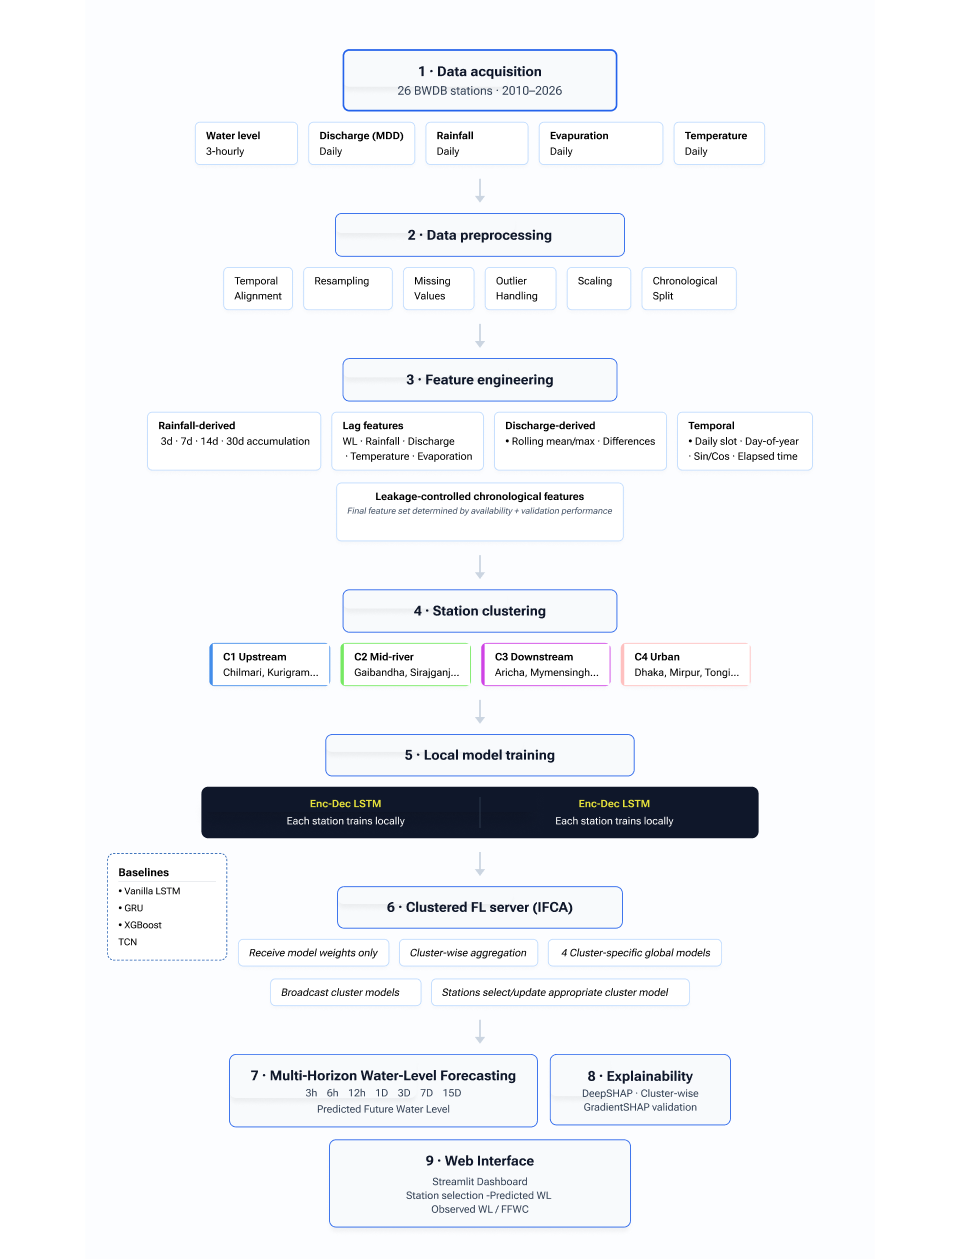
\includegraphics[
        width=0.92\textwidth
    ]{figures2/fig3-1-framework.png}

    \caption{Overall CFL-EDLSTM framework diagram.}
    \label{fig:3.1}
\end{figure}

% ------------------------------------------------------------
\section{Study Area}
\label{sec:3.4}

The study covers 25 water-level monitoring stations distributed across northern, central, western, and Dhaka-metropolitan parts of Bangladesh, spanning a network of 13 named river systems: the Teesta and Dharla in the north; the Deonai-Charalkata-Jamuneswari-Karatoa system; the Brahmaputra-Jamuna mainstem, which contains the largest number of monitoring stations in the study; the Ghagot; the Old Brahmaputra; the interconnected Karatoa-Atrai-Gur-Gumani-Hurasagar system; the Dhaleswari and Kaliganga-Bethua further downstream; and, around the greater Dhaka area, the Buriganga, Turag, Lakhya, and Balu.
BWDB classifies each station as tidal or non-tidal: 5 of the 25 stations, all of them in the Urban cluster and located on the Buriganga, Turag, Lakhya, and Balu channels around Dhaka, are tidal; the remaining 20 are non-tidal. This distinction is reported here as descriptive context about the study area rather than as a formal input to the clustering procedure itself, which is defined separately in \S\ref{sec:3.10.1}.

\setcounter{table}{-1}
\begin{table}[htbp]
  \centering
  \caption{River System Distribution}
  \label{tab:3.0}
  \small
  \begin{tabular}{@{}L{5.0cm} C{1.7cm} L{3.8cm} L{2.2cm}@{}}
    \toprule
    \textbf{River System} & \textbf{No. of Stations} & \textbf{General Location} & \textbf{Tidal Status} \\
    \midrule
    Teesta & 2 & Northern Bangladesh & Non-tidal \\
    Dharla & 1 & Northern Bangladesh & Non-tidal \\
    Deonai--Charalkata--Jamuneswari--Karatoa & 3 & Northern Bangladesh & Non-tidal \\
    Brahmaputra--Jamuna & 6 & Northern and central Bangladesh & Non-tidal \\
    Ghagot & 1 & Northern Bangladesh & Non-tidal \\
    Old Brahmaputra & 2 & Central Bangladesh & Non-tidal \\
    Karatoa--Atrai--Gur--Gumani--Hurasagar & 2 & Central and downstream Bangladesh & Non-tidal \\
    Dhaleswari & 2 & Central and downstream Bangladesh & Non-tidal \\
    Kaliganga--Bethua & 1 & Central and downstream Bangladesh & Non-tidal \\
    Buriganga & 1 & Greater Dhaka & Tidal \\
    Turag & 1 & Greater Dhaka & Tidal \\
    Lakhya & 2 & Greater Dhaka & Tidal \\
    Balu & 1 & Greater Dhaka & Tidal \\
    \midrule
    \textbf{Total} & \textbf{25} & \textbf{Bangladesh} & \textbf{20 Non-tidal / 5 Tidal} \\
    \bottomrule
  \end{tabular}
\end{table}


\begin{figure}[htbp]
    \centering
    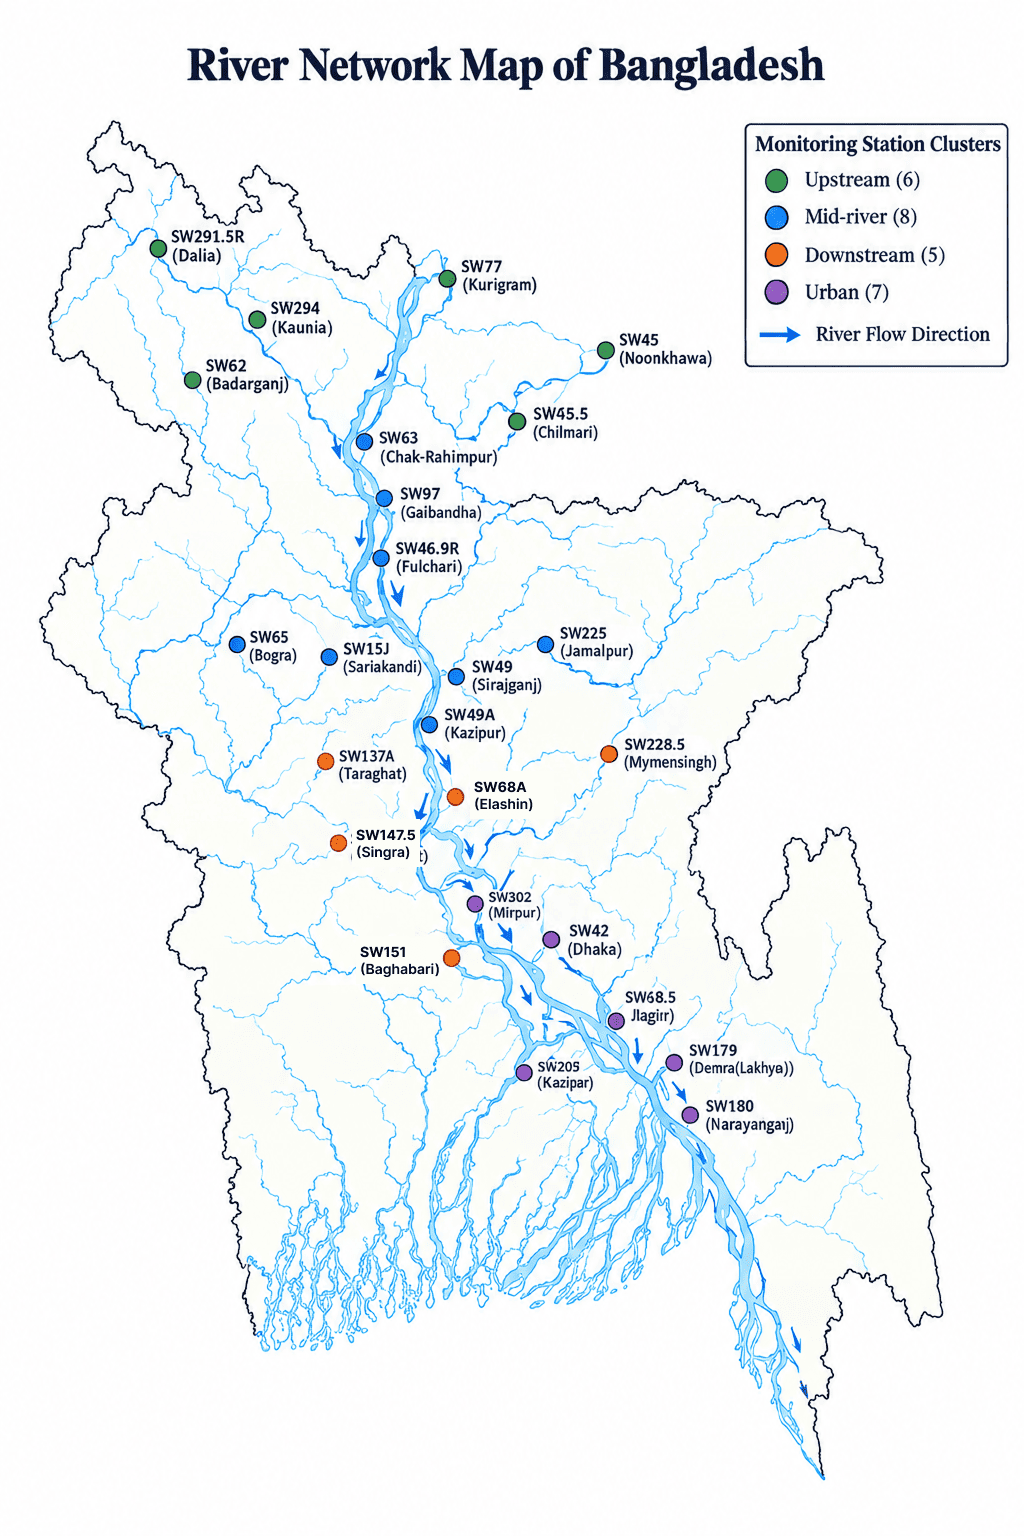
\includegraphics[
        width=0.85\textwidth
    ]{figures2/fig3-2a-river-connectivity.png}

    \caption{River system connectivity within the study area.}
    \label{fig:3.2a}
\end{figure}

\begin{figure}[htbp]
    \centering
    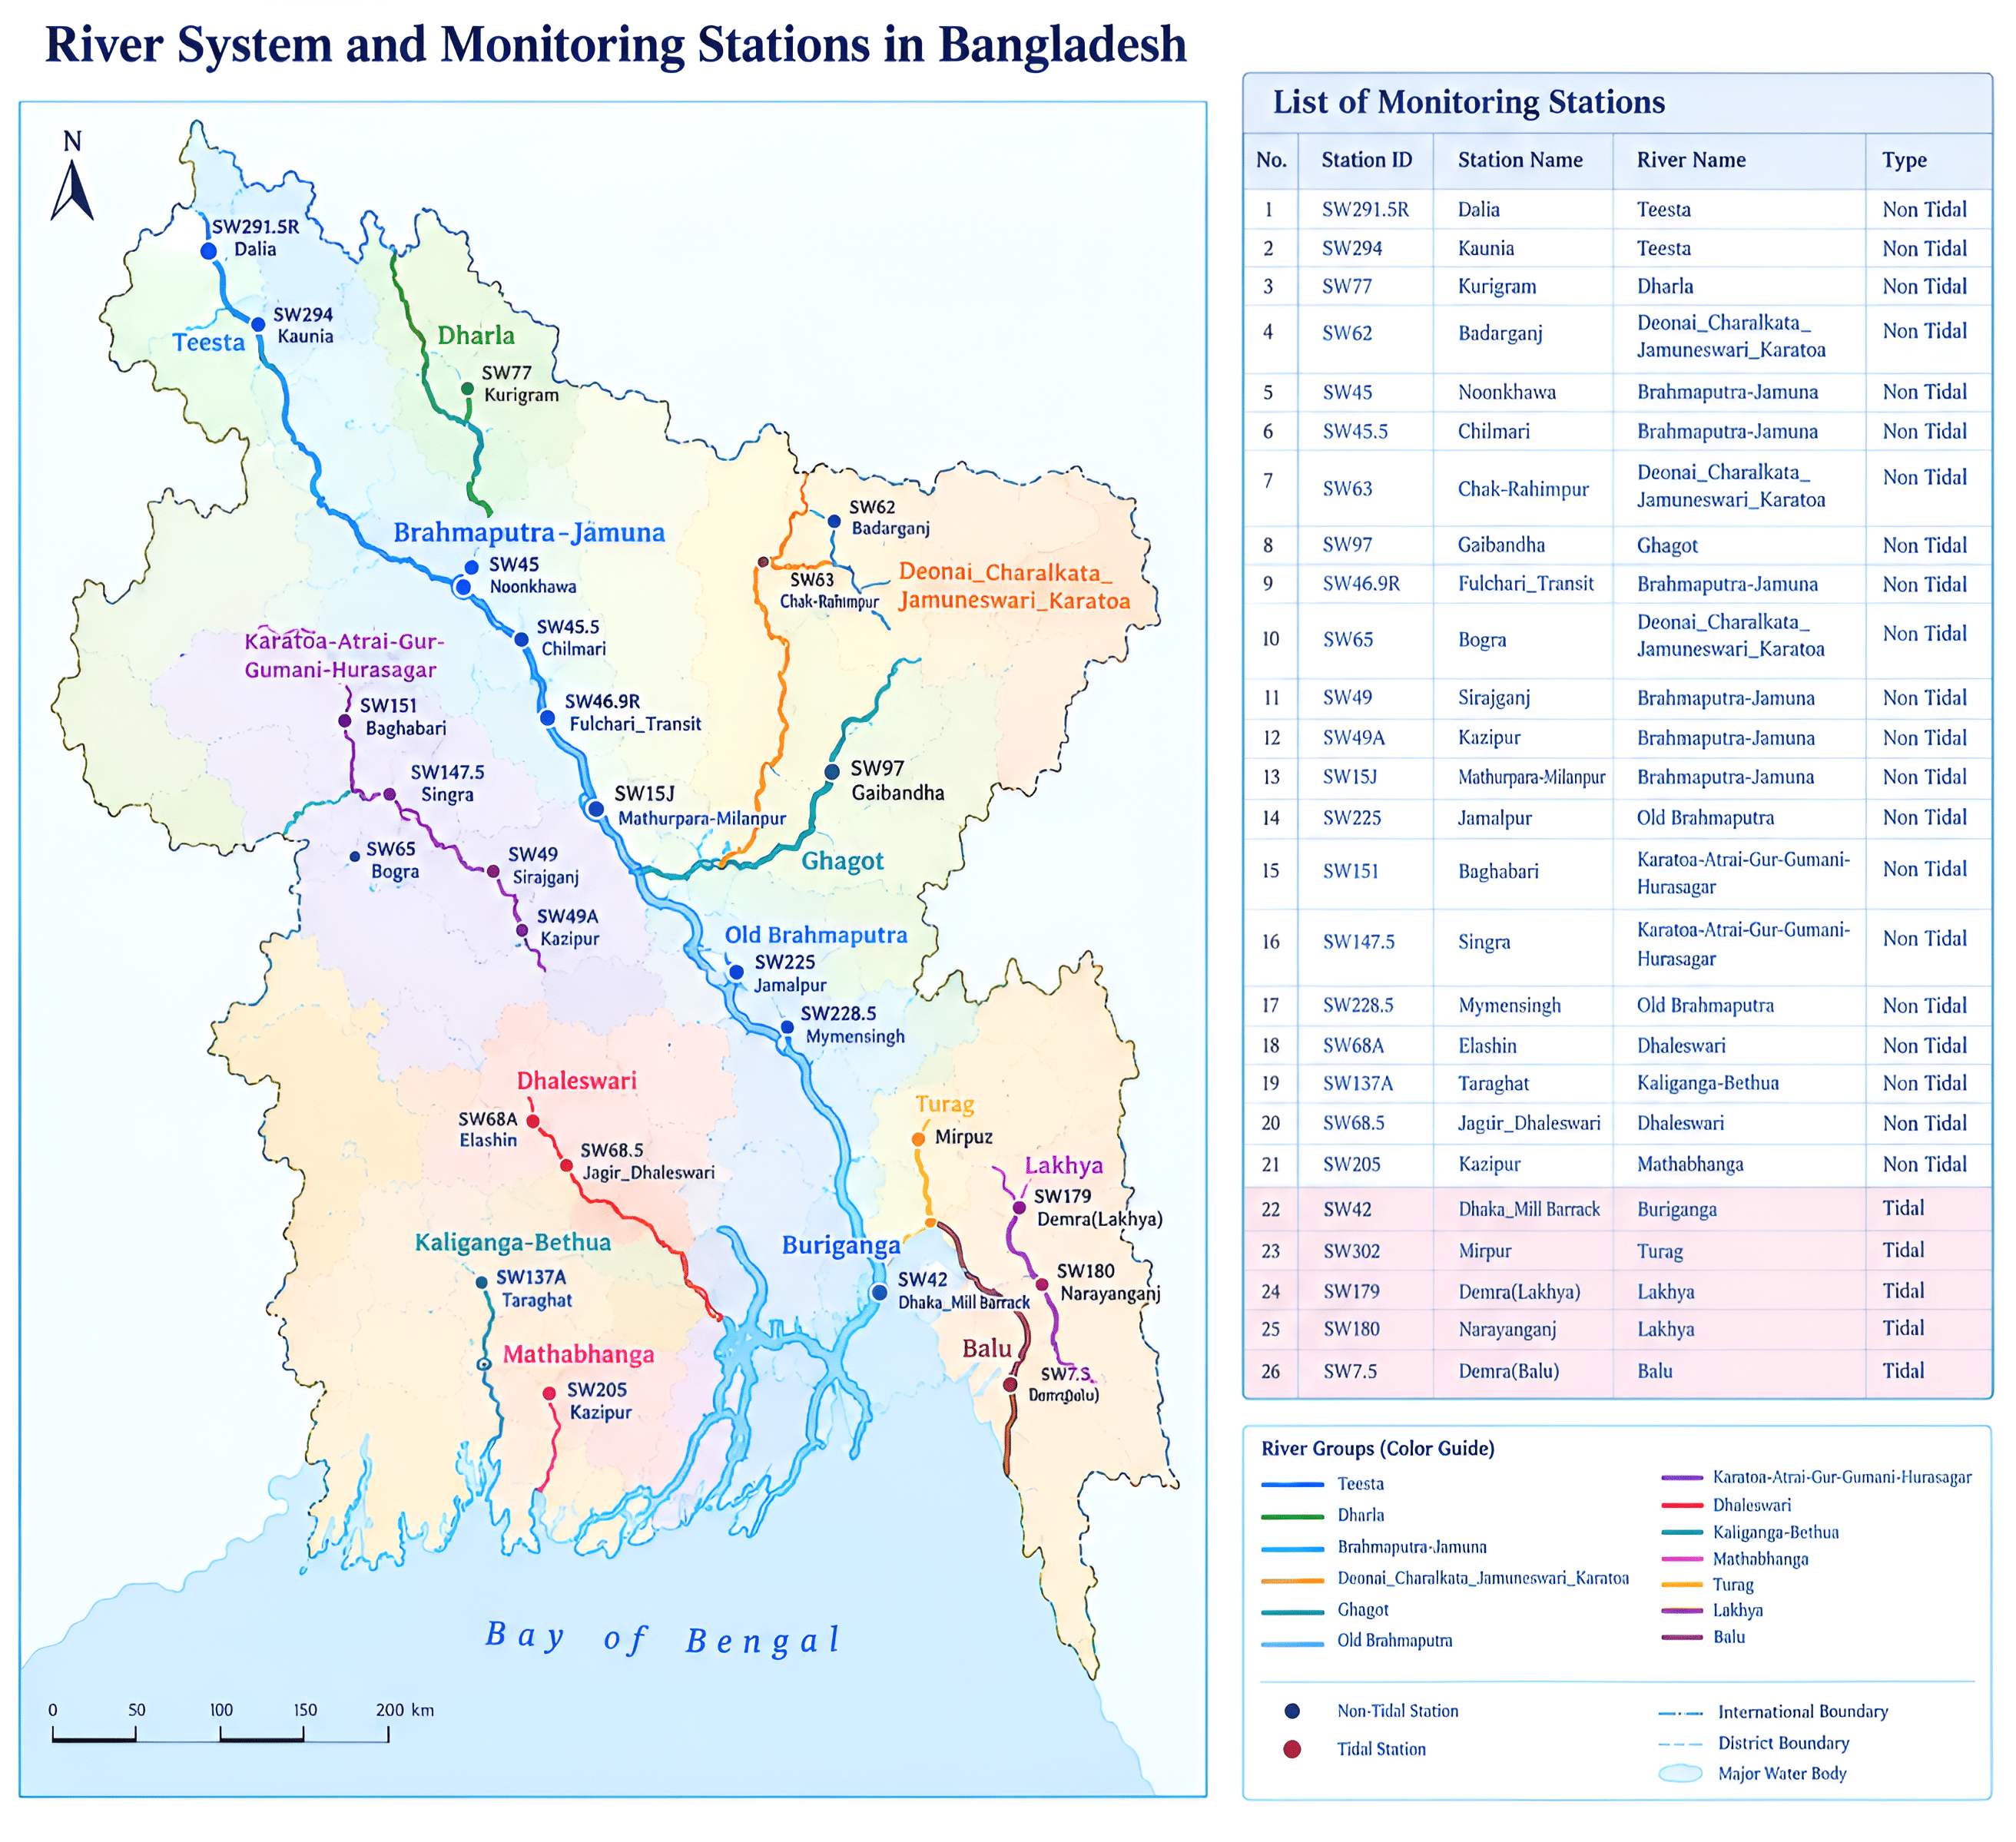
\includegraphics[
        width=0.75\textwidth
    ]{figures2/fig3-2b-station-distribution.png}

    \caption{Geographical distribution of the 25 monitoring stations.}
    \label{fig:3.2b}
\end{figure}

% ------------------------------------------------------------
\section{Monitoring Stations}
\label{sec:3.5}

Water level is the variable with the widest coverage in this study and effectively defines the station network: 25 stations report water level, and every other variable is a subset of that same 25. Table~\ref{tab:3.1} lists them.

\begin{landscape}
\begin{table}[htbp]
  \centering
  \caption{Station Inventory}
  \label{tab:3.1}
  \scriptsize
  \setlength{\tabcolsep}{3pt}
  \begin{tabularx}{\linewidth}{@{}c l X X l X X r r l@{}}
    \toprule
    \textbf{\#} & \textbf{Station ID} & \textbf{Station Name} & \textbf{River} & \textbf{Type} &
    \textbf{District} & \textbf{Upazila} & \textbf{Lat} & \textbf{Long} & \textbf{Cluster} \\
    \midrule
    1 & SW291.5R & Dalia & Teesta & Non-Tidal & Nilphamari & Dimla & 26.176 & 89.051 & Upstream \\
    2 & SW294 & Kaunia & Teesta & Non-Tidal & Rangpur & Kaunia & 25.789 & 89.439 & Upstream \\
    3 & SW77 & Kurigram & Dharla & Non-Tidal & Kurigram & Kurigram Sadar & 25.823 & 89.665 & Upstream \\
    4 & SW62 & Badarganj & Deonai-Charalkata-Jamuneswari-Karatoa & Non-Tidal & Rangpur & Badarganj & 25.682 & 89.076 & Upstream \\
    5 & SW45 & Noonkhawa & Brahmaputra-Jamuna & Non-Tidal & Kurigram & Kurigram Sadar & 25.920 & 89.770 & Upstream \\
    6 & SW45.5 & Chilmari & Brahmaputra-Jamuna & Non-Tidal & Kurigram & Chilmari & 25.568 & 89.679 & Upstream \\
    7 & SW63 & Chak-Rahimpur & Deonai-Charalkata-Jamuneswari-Karatoa & Non-Tidal & Gaibandha & Gobindaganj & 25.147 & 89.360 & Middle \\
    8 & SW97 & Gaibandha & Ghagot & Non-Tidal & Gaibandha & Gaibandha Sadar & 25.339 & 89.551 & Middle \\
    9 & SW46.9R & Fulchari (Transit) & Brahmaputra-Jamuna & Non-Tidal & Gaibandha & Fulchhari & 25.187 & 89.599 & Middle \\
    10 & SW65 & Bogra & Deonai-Charalkata-Jamuneswari-Karatoa & Non-Tidal & Bogura & Bogura Sadar & 24.846 & 89.379 & Middle \\
    11 & SW49 & Sirajganj & Brahmaputra-Jamuna & Non-Tidal & Sirajganj & Sirajganj Sadar & 24.468 & 89.720 & Middle \\
    12 & SW49A & Kazipur & Brahmaputra-Jamuna & Non-Tidal & Sirajganj & Kazipur & 24.670 & 89.649 & Middle \\
    13 & SW15J & Mathurpara-Milanpur & Brahmaputra-Jamuna & Non-Tidal & Bogura & Shariakandi & 24.837 & 89.587 & Middle \\
    14 & SW225 & Jamalpur & Old Brahmaputra & Non-Tidal & Jamalpur & Jamalpur Sadar & 24.922 & 89.968 & Middle \\
    15 & SW151 & Baghabari & Karatoa-Atrai-Gur-Gumani-Hurasagar & Non-Tidal & Sirajganj & Shahjadpur & 24.131 & 89.581 & Downstream \\
    16 & SW147.5 & Singra & Karatoa-Atrai-Gur-Gumani-Hurasagar & Non-Tidal & Natore & Singra & 24.498 & 89.139 & Downstream \\
    17 & SW228.5 & Mymensingh & Old Brahmaputra & Non-Tidal & Mymensingh & Mymensingh Sadar & 24.737 & 90.430 & Downstream \\
    18 & SW68A & Elashin & Dhaleswari & Non-Tidal & Tangail & Delduar & 24.119 & 89.888 & Downstream \\
    19 & SW137A & Taraghat & Kaliganga-Bethua & Non-Tidal & Manikganj & Ghior & 23.858 & 89.956 & Downstream \\
    20 & SW68.5 & Jagir (Dhaleswari) & Dhaleswari & Non-Tidal & Manikganj & Manikganj Sadar & 23.879 & 90.025 & Urban \\
    21 & SW42 & Dhaka (Mill Barrack) & Buriganga & Tidal & Dhaka & Dhaka Sadar (Kotwali) & 23.697 & 90.420 & Urban \\
    22 & SW302 & Mirpur & Turag & Tidal & Dhaka & Mirpur & 23.785 & 90.336 & Urban \\
    23 & SW179 & Demra (Lakhya) & Lakhya & Tidal & Dhaka & Demra & 23.728 & 90.506 & Urban \\
    24 & SW180 & Narayanganj & Lakhya & Tidal & Narayanganj & Narayanganj Sadar & 23.630 & 90.515 & Urban \\
    25 & SW7.5 & Demra (Balu) & Balu & Tidal & Dhaka & Demra & 23.733 & 90.496 & Urban \\
    \bottomrule
  \end{tabularx}
\end{table}
\end{landscape}




% \begin{figure}[htbp]
%     \centering

%     \includegraphics[
%         width=0.85\textwidth
%     ]{figures/fig3-3-cluster-map.png}

%     \caption{25-station, four-cluster spatial map of Bangladesh.}
%     \label{fig:3.3}
% \end{figure}

% ------------------------------------------------------------
\section{Data Sources}
\label{sec:3.6}

\begin{landscape}
\begin{table}[htbp]
  \centering
  \caption{Data Sources by Variable}
  \label{tab:3.2}
  \footnotesize
  \setlength{\tabcolsep}{4pt}
  \renewcommand{\arraystretch}{1.25}
  \begin{tabularx}{\linewidth}{@{}L{2.0cm} L{1.3cm} L{1.9cm} X L{2.2cm} L{1.3cm}@{}}
    \toprule
    \textbf{Variable} & \textbf{Source} & \textbf{Station Coverage} &
    \textbf{How Used} & \textbf{Collection Period} & \textbf{Unit} \\
    \midrule
    Water Level & BWDB gauge stations & 25 stations &
    Retained at native 5-obs/day resolution as the study's master timeline (\S\ref{sec:3.9.3}) &
    1 Jan 2010 -- 31 Mar 2026 & WL (mMSL) \\

    Discharge & BWDB & 15 stations &
    Used directly + trend features; mapped across the 5 WL slots per date &
    1 Jan 2010 -- 31 Dec 2024 & MDD (m\textsuperscript{3}/s) \\

    Rainfall & BWDB / BMD & 13 stations &
    Used directly + cumulative windows; mapped across the 5 WL slots per date &
    1 Jan 2010 -- $\sim$30 Apr 2026 & mm \\

    Temperature & Mendeley dataset + NASA POWER & 11 districts (district-level) &
    Gaps filled via interpolation, mapped to stations by district, then mapped across the 5 WL slots &
    2012 -- 2024 & \textdegree C \\

    Evaporation & BWDB & 7 stations (station-level) &
    Linearly interpolated to fill gaps; mapped across the 5 WL slots per date &
    1 Jan 2010 -- 28 Feb 2026 & mm/day \\
    \bottomrule
  \end{tabularx}
\end{table}
\end{landscape}

Not every station carries every variable. Water level has by far the widest footprint, at 25 stations; evaporation is the narrowest, at 7. Temperature is district-level rather than station-level, so it has to be mapped onto individual stations by district rather than read directly from a gauge --- this is discussed further in \S\ref{sec:3.9.1} and \S\ref{sec:3.9.3}.

% ------------------------------------------------------------
\section{Dataset Description}
\label{sec:3.7}

Across the five variables, the dataset totals 1,092,687 raw observations before any cleaning or alignment: 762,813 for water level, 46,812 for discharge, 71,110 for rainfall, 40,761 for evaporation, and 171,191 for temperature. Water level's much larger share reflects both its wider station coverage and its finer native resolution (5 observations/day, against daily for discharge, rainfall, temperature, and evaporation).

Coverage across variables is genuinely uneven rather than a uniform grid. Of the 13 districts represented anywhere in the dataset, only four --- Bogura, Dhaka, Rangpur, and Sirajganj --- have all five variables present. Most districts have three or four, and one (Narayanganj) have only water level and one other variable. This unevenness is exactly why station clustering (\S\ref{sec:3.10}) and careful preprocessing (\S\ref{sec:3.9}) matter as much as they do here --- a model can't assume every station looks like every other station going in.

% ------------------------------------------------------------
\section{Input and Target Variables}
\label{sec:3.8}

Five variables make up the modeling input, one of which --- water level --- is also the forecasting target. Combining them this way directly answers the single-variable limitation flagged repeatedly in Chapter~2 \cite{Islam2026b,Ruma2023,Rakin2023,HemelSakib2024}, none of which brought discharge, water level, rainfall, temperature, and evaporation together in one framework.

\begin{table}[htbp]
  \centering
  \caption{Input and Target Variables}
  \label{tab:3.3}
  \small
  \renewcommand{\arraystretch}{1.2}
  \setlength{\tabcolsep}{5pt}
  \begin{tabular}{@{}L{2.1cm} L{2.2cm} L{4.0cm} L{2.7cm} L{1.7cm}@{}}
    \toprule
    \textbf{Variable} & \textbf{Type} & \textbf{Original Resolution} & \textbf{Role} & \textbf{Unit} \\
    \midrule
    Water Level & Hydrological & 3-hourly, 5 obs/day (06:00--18:00) & Target (and input, via lag) & mMSL \\
    Discharge & Hydrological & Daily (mean) & Input & m\textsuperscript{3}/s (MDD) \\
    Rainfall & Meteorological & Daily & Input & mm \\
    Temperature & Meteorological & Daily (district-level) & Input & \textdegree C \\
    Evaporation & Meteorological & Daily (with gaps) & Input & mm/day \\
    \bottomrule
  \end{tabular}
\end{table}

\subsection{Water Level}
\label{sec:3.8.1}

Water level is the target variable throughout this thesis. It is recorded at 25 BWDB gauge stations five times a day --- 06:00, 09:00, 12:00, 15:00, and 18:00, three hours apart during the day with a twelve-hour gap overnight --- the finest native resolution of any variable in the dataset, and it is retained at that native resolution as the study's master modelling timeline (\S\ref{sec:3.9.3}), rather than being collapsed down to a single daily value. Measured in metres above mean sea level (mMSL), it is the quantity every forecast horizon in this thesis ultimately predicts, following the same target-variable choice made by \cite{Ruma2023} and, for a smaller station set, \cite{Islam2026b}.

\subsection{Discharge}
\label{sec:3.8.2}

Discharge (mean daily discharge, MDD) is recorded at 15 of the 25 stations, in cubic metres per second, and used both directly and through derived trend features. Discharge is the input variable \cite{Islam2026a} relied on exclusively for their Old Brahmaputra forecasting work --- and one of the two limitations they themselves flagged was the exclusion of exactly the kind of meteorological variables (rainfall, temperature) this thesis adds alongside it.

\subsection{Rainfall}
\label{sec:3.8.3}

Rainfall is recorded daily at 13 stations, in millimetres, and used both directly and as cumulative windows to capture delayed catchment response. This mirrors the lag-based and cumulative-rainfall treatment used by \cite{Islam2026b} and the areal-rainfall approach of \cite{Cui2022}, both of which found rainfall to carry real, if secondary, predictive weight relative to antecedent discharge or water level.

\subsection{Temperature}
\label{sec:3.8.4}

Temperature is the one variable in this dataset that is not station-specific: it comes from a combination of a Mendeley dataset and NASA POWER reanalysis data, at daily resolution, covering 11 districts, with gaps filled via interpolation and values mapped onto stations by district. Because temperature is district-level rather than station-level, it still carries less direct/observational weight than the station-specific variables, and any gap-filling interpolation should be treated with the same caution as elsewhere in the dataset --- worth being explicit about in any later discussion of SHAP-based feature importance (\S3.16 / Chapter~4), since a variable mapped from district to station shouldn't be interpreted quite the same way as one measured directly at the station.

\subsection{Evaporation}
\label{sec:3.8.5}

Evaporation is recorded daily at 7 stations --- the narrowest coverage of any variable --- and, like temperature, is linearly interpolated to daily values where gaps exist. Its inclusion follows the precedent of \cite{Cui2022}, who found that adding evaporation alongside rainfall improved multi-step forecasting accuracy in their Encoder--Decoder framework, even though its coverage in that study was similarly narrower than the other inputs.

% ------------------------------------------------------------
\section{Data Preprocessing}
\label{sec:3.9}

\begin{figure}[htbp]
    \centering

    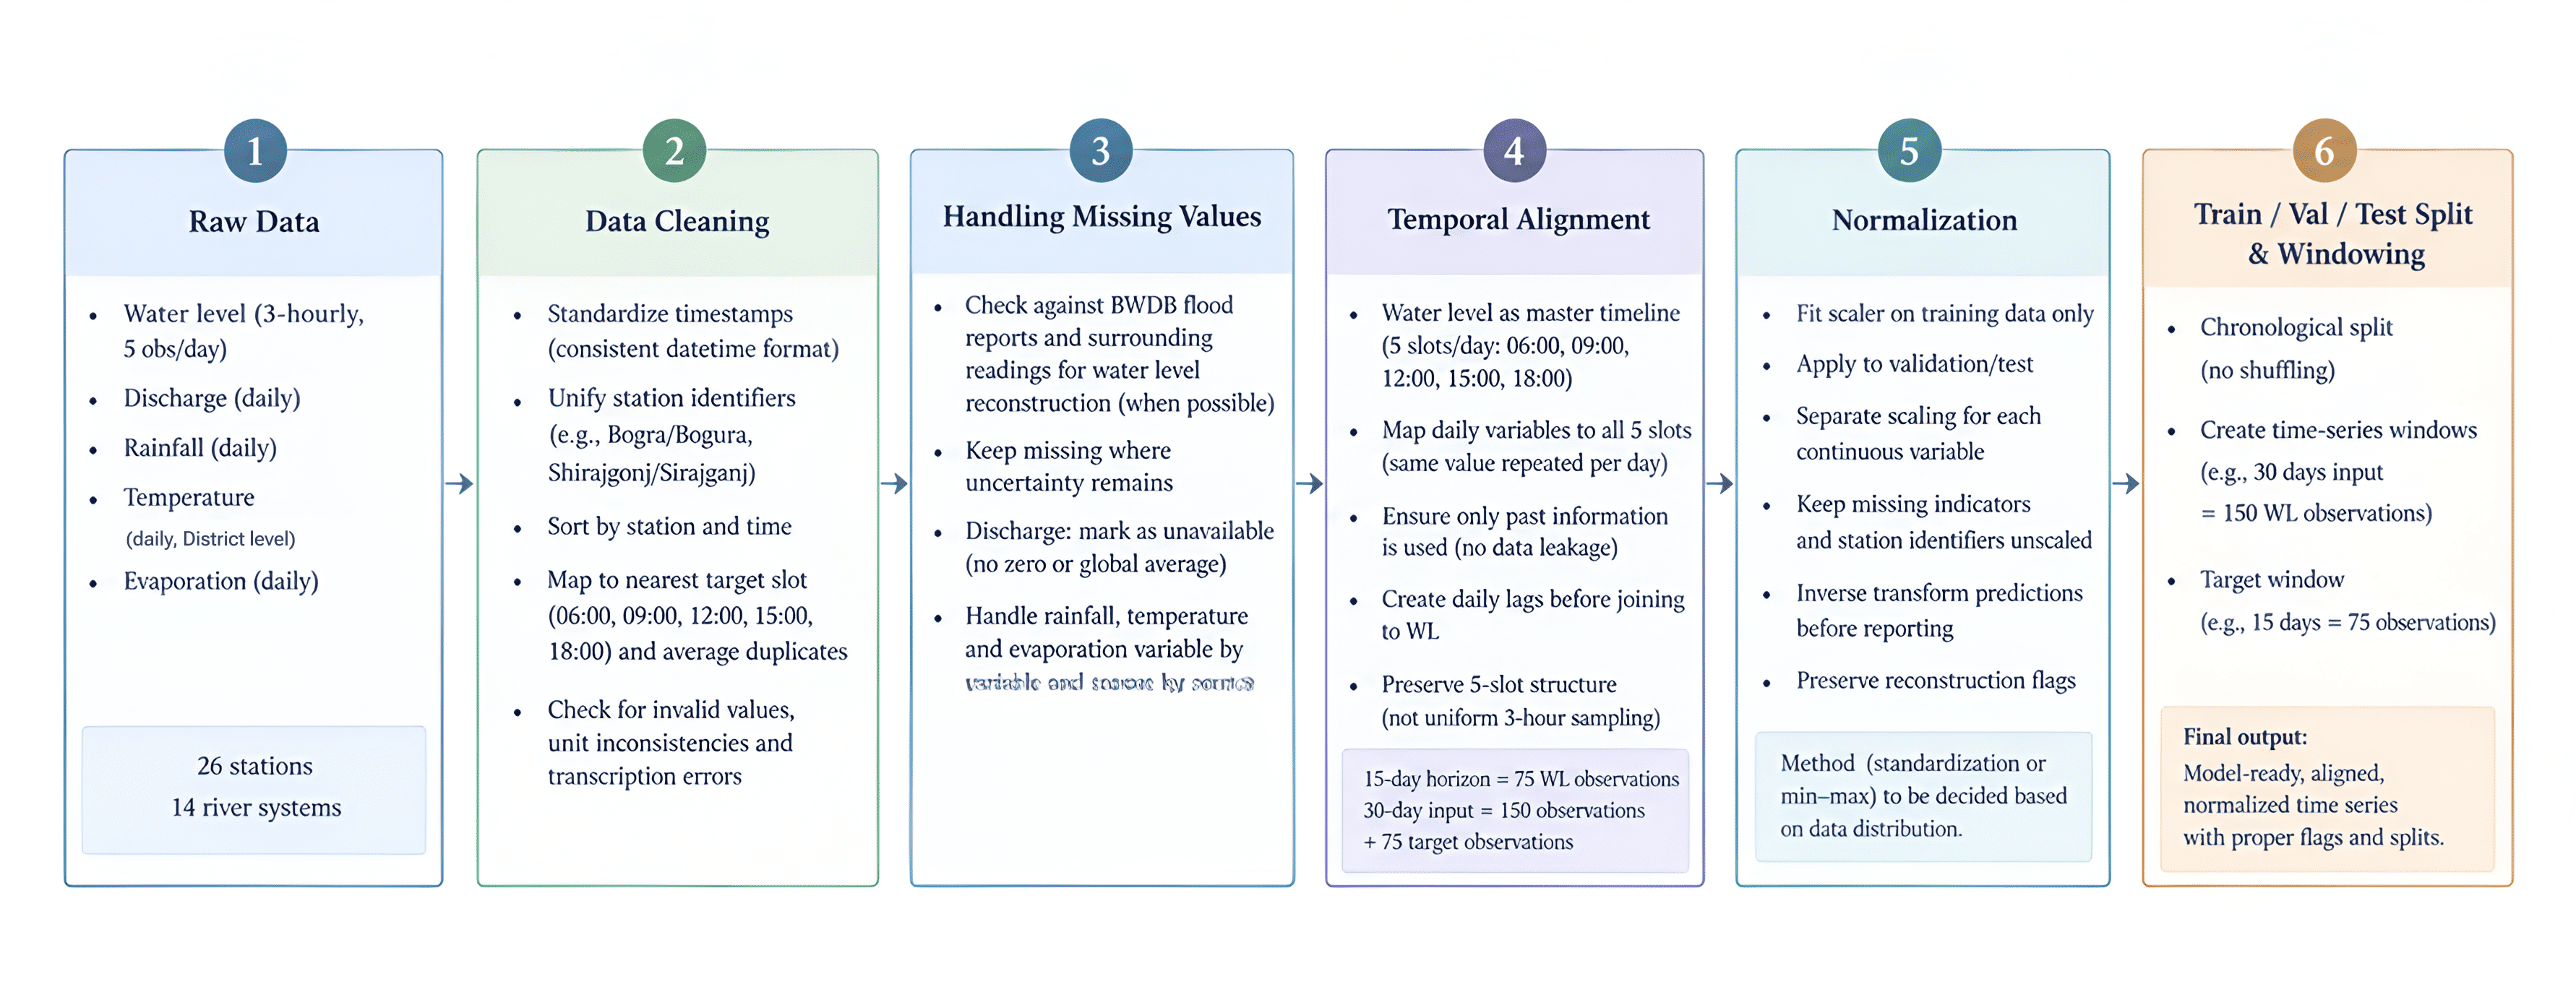
\includegraphics[
        width=0.9\textwidth
    ]{figures2/fig3-4-preprocessing-pipeline.png}

    \caption{Data preprocessing pipeline flowchart.}
    \label{fig:3.4}
\end{figure}

\subsection{Data Cleaning}
\label{sec:3.9.1}

Before anything else, timestamps across all five sources are parsed into one consistent datetime format, station identifiers are standardized against the naming inconsistencies already flagged in \S\ref{sec:3.5} (Bogra/Bogura, Shirajgonj/Sirajganj, and similar), and every record is sorted by station and time. Water-level readings are mapped to the nearest of the five target slots --- 06:00, 09:00, 12:00, 15:00, or 18:00 --- by closest value alone, with no separate tolerance threshold applied. Where more than one reading lands in the same station-slot, they're combined by taking the mean. Duplicate records, impossible numeric values, inconsistent units, and likely transcription errors are all checked for --- but extreme water-level values are inspected rather than dropped automatically, since an extreme reading during this kind of study is just as likely to be a real flood as it is to be an error.

Before any of the four supporting variables get merged in, the station metadata itself is checked. Rainfall, temperature, and evaporation are assigned to the 25 water-level stations primarily by district match --- whatever district a station is recorded under is used to find the corresponding rainfall/temperature/evaporation source for that same district --- and where no matching source exists in that station's own district, the nearest available station geographically is used instead. Discharge (MDD) is mapped directly to its corresponding water-level station wherever a measurement exists. Which source gauge fed which station is kept on record throughout, rather than discarded once the merge is done.

\subsection{Handling Missing Values}
\label{sec:3.9.2}

Missing water-level readings aren't treated as random noise. A large share of them are almost certainly tied to flooding itself, since gauges can fail or go unread precisely when water levels spike --- which means the gaps that matter most are exactly the ones a careless imputation method would handle worst. Where a gap coincides with a known event, it's checked against BWDB flood reports and the surrounding water-level trajectory at that station, and only reconstructed where both the report and the neighboring readings genuinely support a specific value --- with reconstructed points flagged separately from directly observed ones from that point on. Where the evidence isn't strong enough to reconstruct with any confidence, the gap stays marked as missing rather than being papered over.

Discharge is handled more conservatively, since it maps directly to specific stations and simply isn't available at all of them. A missing MDD value is recorded as unavailable, never as zero, and is never filled in from a global average or borrowed from another station. Gaps in rainfall, temperature, and evaporation are handled on the same principle --- assessed variable by variable and source by source.

One station needs an explicit note rather than silent handling: the Narayanganj Sadar rainfall record contains only 61 entries, against roughly 5,900 for every other rainfall station. It is retained in the dataset --- removing it now would require re-touching totals and figures already finalized elsewhere in this thesis, and no alternative or supplementary source is currently available for it --- but its extremely limited coverage means it should be treated with caution in any rainfall-dependent feature or result specific to that station, and this limitation is stated explicitly here rather than left for a reader to discover on their own.

\subsection{Temporal Alignment}
\label{sec:3.9.3}

Water level defines the modelling timeline here, at its native five-observations-a-day schedule (06:00, 09:00, 12:00, 15:00, 18:00), rather than being collapsed down to a single daily value. The four supporting variables --- rainfall, temperature, evaporation, and discharge --- are all daily, so each one is mapped to its corresponding station and matched by date across all five of that date's water-level slots; a given day's rainfall total, for instance, appears identically in all five rows for that date. That repetition is there to align the feature matrix, not to imply five independent rainfall measurements were actually taken.

The definition and reporting window of each daily variable are checked before use. A daily total that includes measurements occurring after a WL prediction time must not be treated as already known at that time. Inputs must reflect only information available at the forecast origin. Where suitable, daily lags are generated by shifting the original daily series by calendar days before joining it to WL, rather than shifting rows in the expanded five-observation dataset.

Daytime observations are approximately three hours apart, but the interval from 18:00 to the following 06:00 is twelve hours. The series is therefore not uniformly sampled every three hours. Preprocessing preserves the five-slot daily structure or represents elapsed time explicitly where supported by the model. A 15-day horizon corresponds to 75 WL observations; for example, a 30-day input window contains 150 WL observations followed by a 75-observation target.


\begin{figure}[htbp]
    \centering

    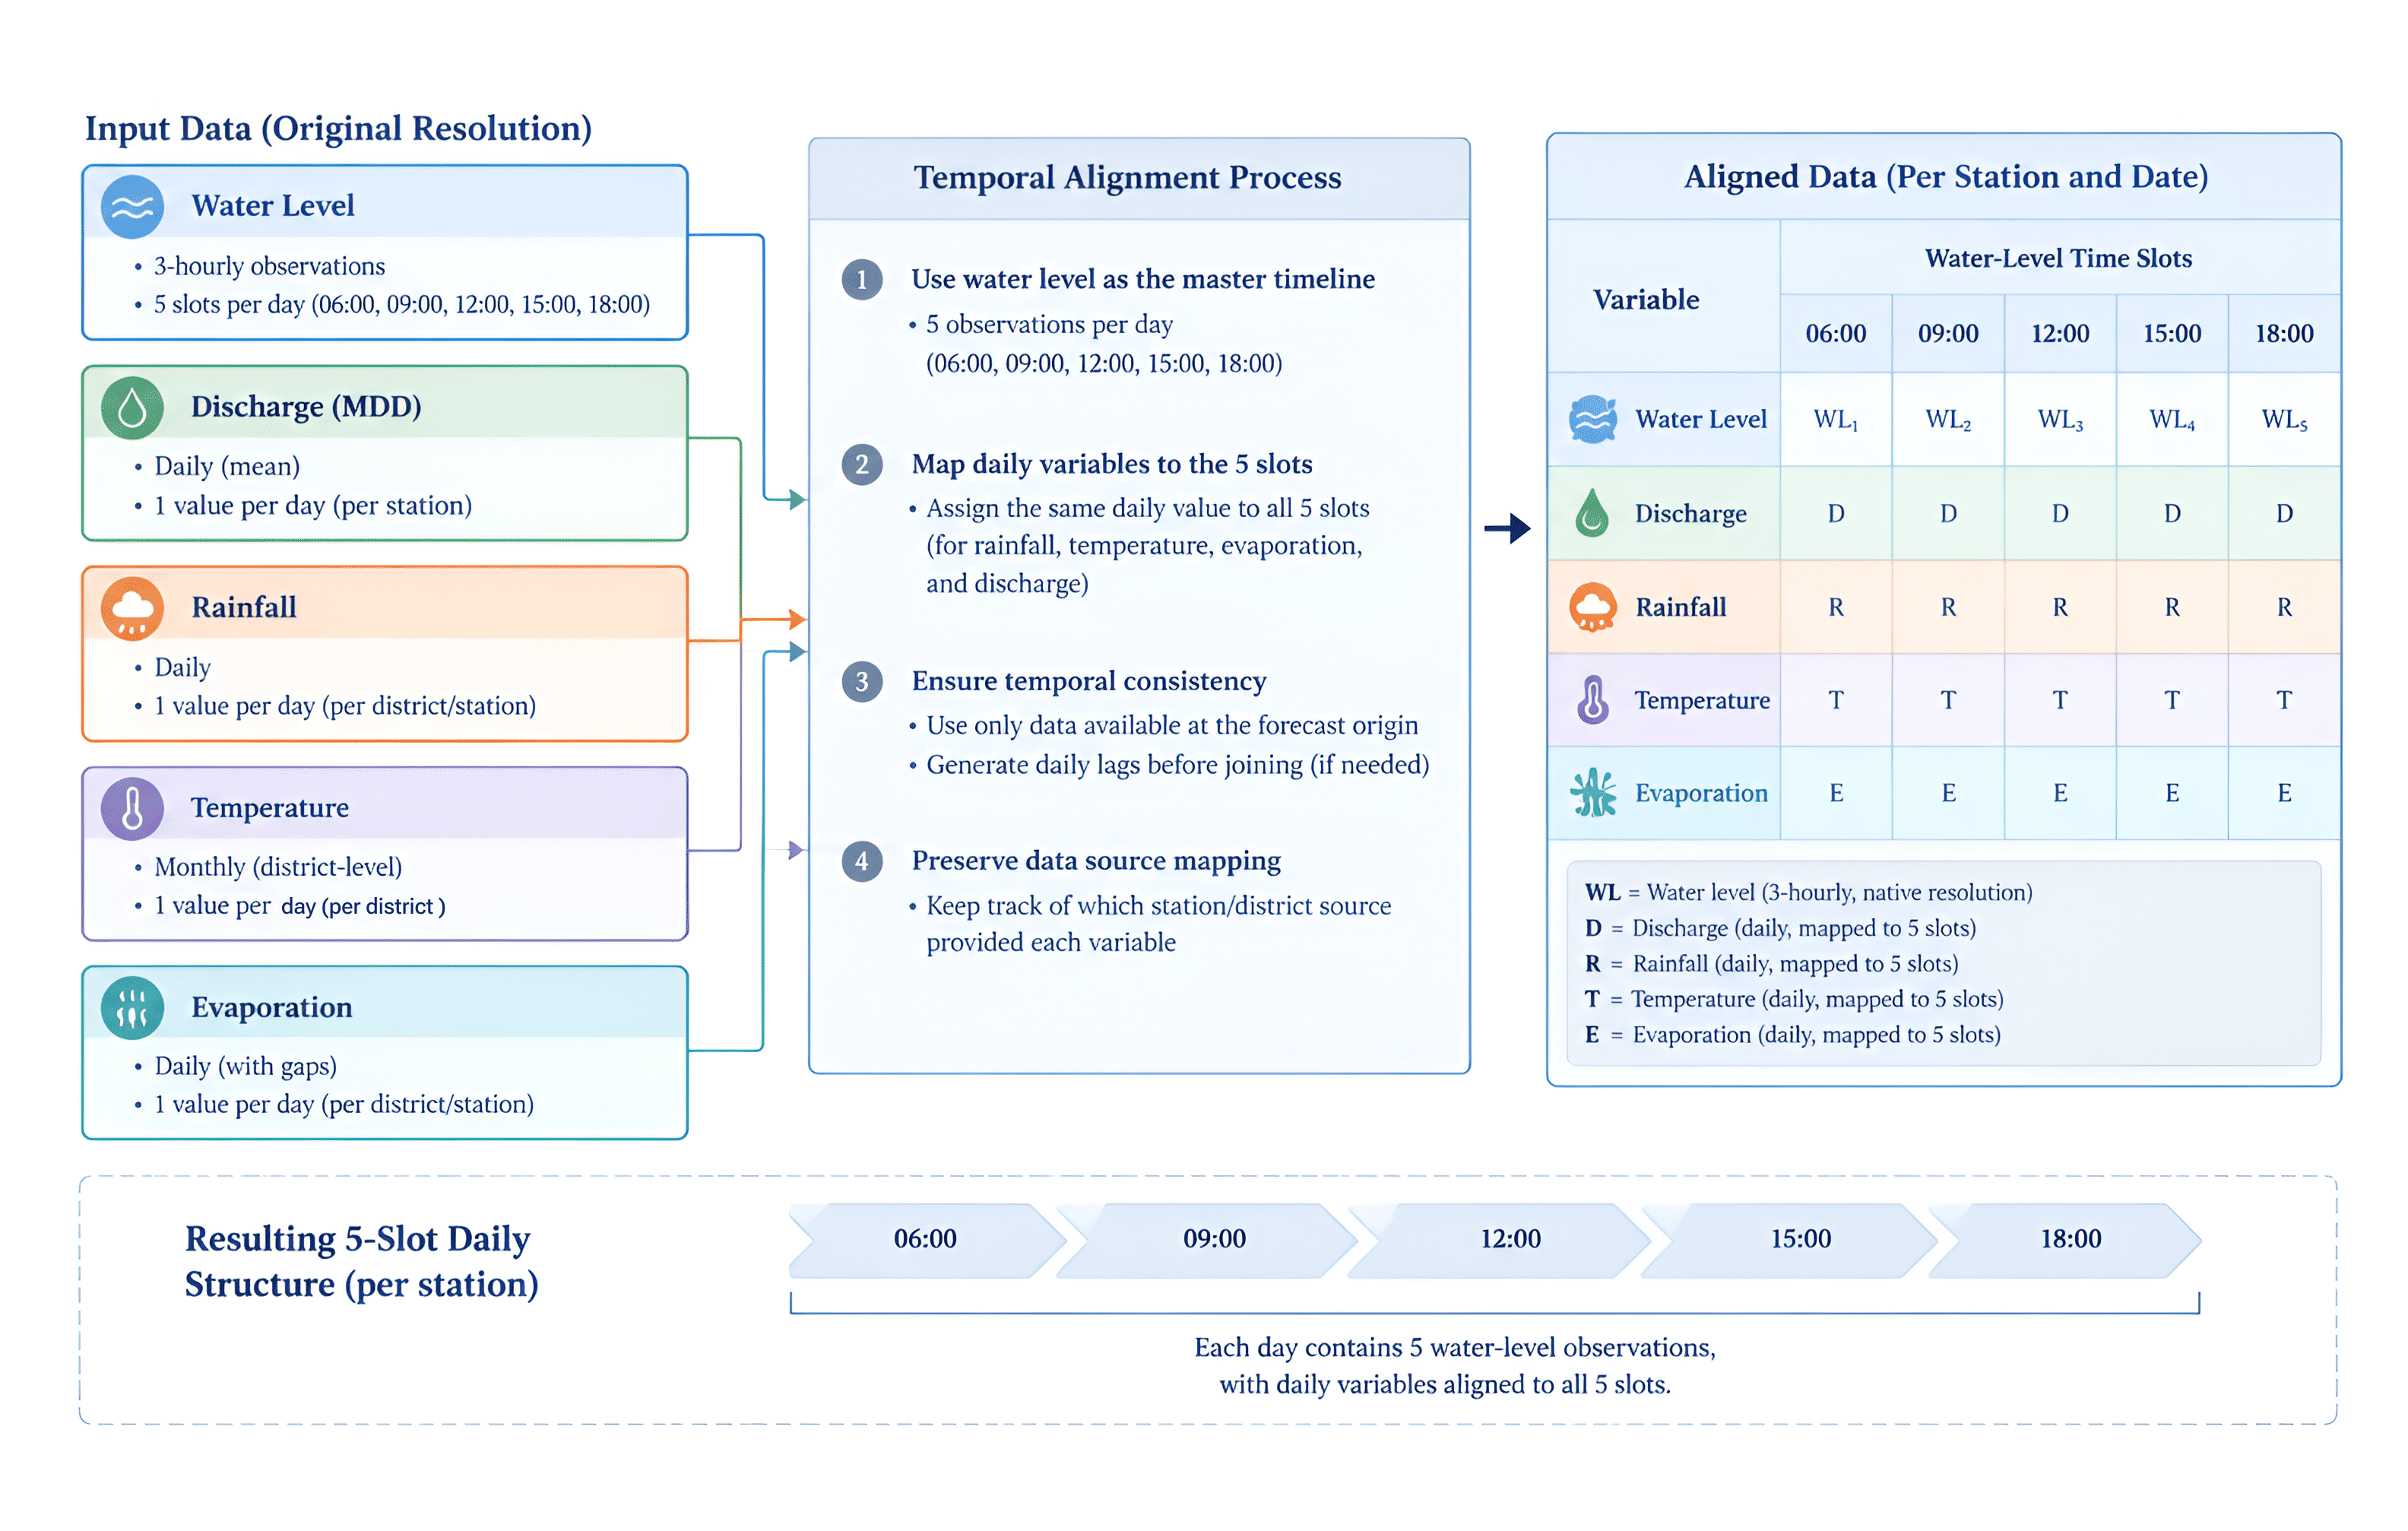
\includegraphics[
        width=0.9\textwidth
    ]{figures2/fig3-5-temporal-alignment.png}

    \caption{Temporal alignment and data-resolution diagram.}
    \label{fig:3.5}
\end{figure}

\begin{table}[htbp]
  \centering
  \caption{Preprocessing Summary}
  \label{tab:3.4}
  \small
  \renewcommand{\arraystretch}{1.2}
  \begin{tabular}{@{}L{2.1cm} L{2.7cm} L{5.1cm} L{3.1cm}@{}}
    \toprule
    \textbf{Variable} & \textbf{Original Resolution} & \textbf{Processing Applied} & \textbf{Final Resolution} \\
    \midrule
    Water Level & 3-hourly, 5 obs/day (06:00--18:00) &
    Retained at native resolution as the master modelling timeline & 5 obs/day (native) \\

    Discharge & Daily (mean) &
    Used directly; trend/rolling features derived; mapped across the 5 WL slots per date &
    Daily value, mapped to 5 WL slots \\

    Rainfall & Daily &
    Used directly; cumulative/lag features derived; mapped across the 5 WL slots per date &
    Daily value, mapped to 5 WL slots \\

    Temperature & Daily, district-level &
    Gaps filled via interpolation; mapped to stations by district; then mapped across the 5 WL slots &
    Daily value, mapped to 5 WL slots \\

    Evaporation & Daily (with gaps) &
    Linearly interpolated to fill gaps; mapped across the 5 WL slots per date &
    Daily value, mapped to 5 WL slots \\
    \bottomrule
  \end{tabular}
\end{table}

\subsection{Normalization}
\label{sec:3.9.4}

Every continuous variable is scaled before it reaches the model, since stable optimization depends on it. Water level, discharge, rainfall, temperature, and evaporation are all scaled separately, since none of them share units or ranges, and the exact method --- standardization or min--max, consistent with the approaches used by \cite{Ruma2023} and \cite{Rakin2023} --- will be chosen once the actual data distributions are in front of us rather than picked in advance. Whether water level needs station-wise scaling is still an open question too; if local baselines differ enough between stations, scaling per station may be worth it, but that decision has to weigh its effect on later cross-station and cross-cluster comparisons, not just on model convergence.

Whatever method is chosen, its parameters are fit on the training data only, then applied unchanged to validation and test. Missingness indicators and station identifiers are left alone rather than scaled as if they were ordinary continuous measurements. Every fitted scaler is saved, predictions are inverse-transformed back into physical units before they're reported, and reconstructed water-level values keep their flag all the way through, so a reconstructed point is never mistaken for a directly observed one downstream.

\subsection{Data Splitting}
\label{sec:3.9.5}

The data is split chronologically, never randomly --- a random split would scatter temporally adjacent, and even future, observations across training and test sets, which defeats the point of a forecasting evaluation. Rather than committing to a single split up front, several chronological configurations are being tried, with the boundary between training, validation, and test moved and re-evaluated to see which split actually yields the most reliable performance, consistent with the chronological (not random) approach used by \cite{Cui2022}. Each candidate boundary is chosen with the same considerations in mind --- what dates are actually available, how station coverage changes across the period, and how flood events are distributed across the timeline --- and whichever configuration is used, it's documented rather than left implicit.

Input and target windows are always built in temporal order, with every target strictly following its input, and the model, scalers, and any imputation parameters are fit using training data alone regardless of which split is being tested. Validation is reserved for model selection, and the test period only ever gets used for a final evaluation. Across all of this, the 15-day horizon (75 water-level observations) is the evaluation point, and errors are reported back in the original water-level units rather than left in scaled form.

\subsection{Feature Engineering}
\label{sec:3.9.6}

Beyond the five raw variables, a set of derived features is built from the cleaned, aligned dataset to make the delayed and cumulative nature of hydrological response more directly visible to the model than the raw series alone would.

\begin{figure}[htbp]
    \centering
    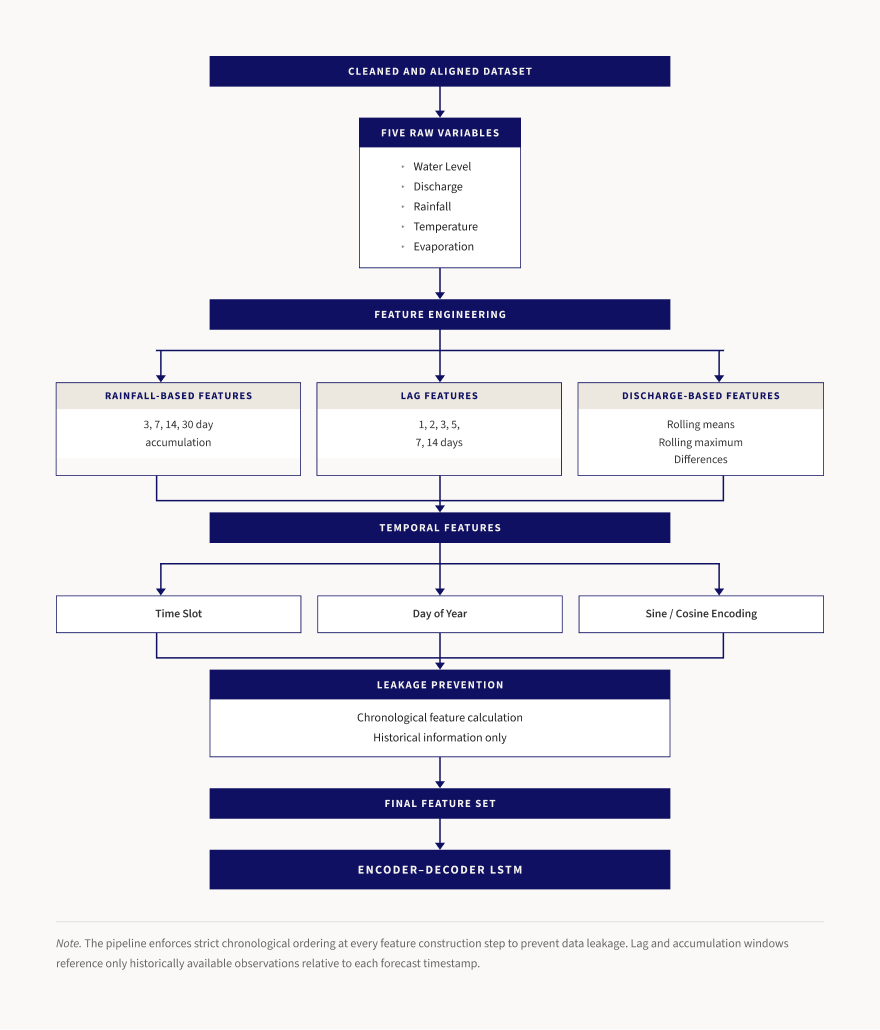
\includegraphics[
        width=0.85\textwidth
    ]{figures2/feature-eng.png}

    \caption{Feature Engineering Workflow}
    \label{fig:3.9.6a}
\end{figure}


\paragraph{Rainfall accumulation.}
To capture how antecedent rainfall builds up before it shows in the river, rainfall is accumulated over look-back windows of 3, 7, 14, and 30 days. For a rainfall series $R$, the accumulated rainfall over the $k$ preceding days is:

\begin{equation}
  R_{\mathrm{acc},k}(t) \;=\; \sum_{i=1}^{k} R(t - i),
  \qquad k \in \{3,\, 7,\, 14,\, 30\}
  \label{eq:3.1}
\end{equation}

which captures both short, sharp rainfall events and longer wet spells, using only rainfall that occurred strictly before the forecast origin.

\paragraph{Lag features.}
Rainfall, discharge, temperature, and evaporation are each given lagged versions at offsets of roughly 1, 2, 3, 5, 7, and 14 days, depending on what the data actually supports, and water-level lags are built from its own preceding observations or matching daily slots. These daily-variable lags are computed on the original daily series first, before that series gets expanded across the five water-level slots --- doing it the other way around would treat five copies of the same value as five independent lags and quietly produce the wrong interval.

\paragraph{Discharge-derived features.}
Recent flow conditions are represented through rolling means of discharge over 3-, 7-, 14-, and, where the data allows, 30-day windows, along with rolling maximum discharge over 7- and 14-day windows to flag recent high-flow periods. One- and three-day discharge differences are also included. None of these are computed where the underlying discharge observations don't meet the completeness rules already set in \S\ref{sec:3.9.2} --- a missing discharge value is never treated as zero for the purpose of building a rolling feature.

\paragraph{Temporal features.}
Calendar and observation-time information is folded in as well --- which of the five daily slots an observation falls in, day of year, and related calendar variables --- with cyclical quantities like time-of-day and day-of-year encoded via sine/cosine transforms. The elapsed time between consecutive observations is also carried through explicitly, given the schedule's own 12-hour overnight gap against the roughly 3-hour daytime gaps established in \S\ref{sec:3.9.3}.

\paragraph{Leakage prevention.}
All of the above is computed strictly chronologically, using only information that would genuinely have been available at each forecast origin. The reporting window of every daily variable is checked specifically for this. The final feature set is decided based on data availability and validation performance, not fixed in advance. The forecasting task itself targets 15 days ahead, or 75 water-level observations under the five-observations-per-day schedule.

% ------------------------------------------------------------
\section{Station Clustering}
\label{sec:3.10}

\subsection{Clustering Criteria}
\label{sec:3.10.1}

Stations were grouped into four clusters using a combination of hydrological/geographic position and a manual cross-check against how stations are actually grouped for operational use on Bangladesh's real-time flood forecasting platform (FFWC). Three factors informed the grouping: position along the river system (upstream tributary, mid-river/mainstem, or downstream distributary reach); proximity to the Dhaka metropolitan area; and, where a station's geographic placement alone was ambiguous, its treatment within FFWC's own operational station groupings, checked and applied manually rather than derived from a statistical clustering algorithm. This domain-knowledge-based approach responds directly to the gap flagged in Chapter~2's review of the general CFL literature \cite{Ghosh2021,Harshvardhan2022,BenAli2026}, none of which were built for a real hydrological network.

\begin{figure}[htbp]
    \centering
    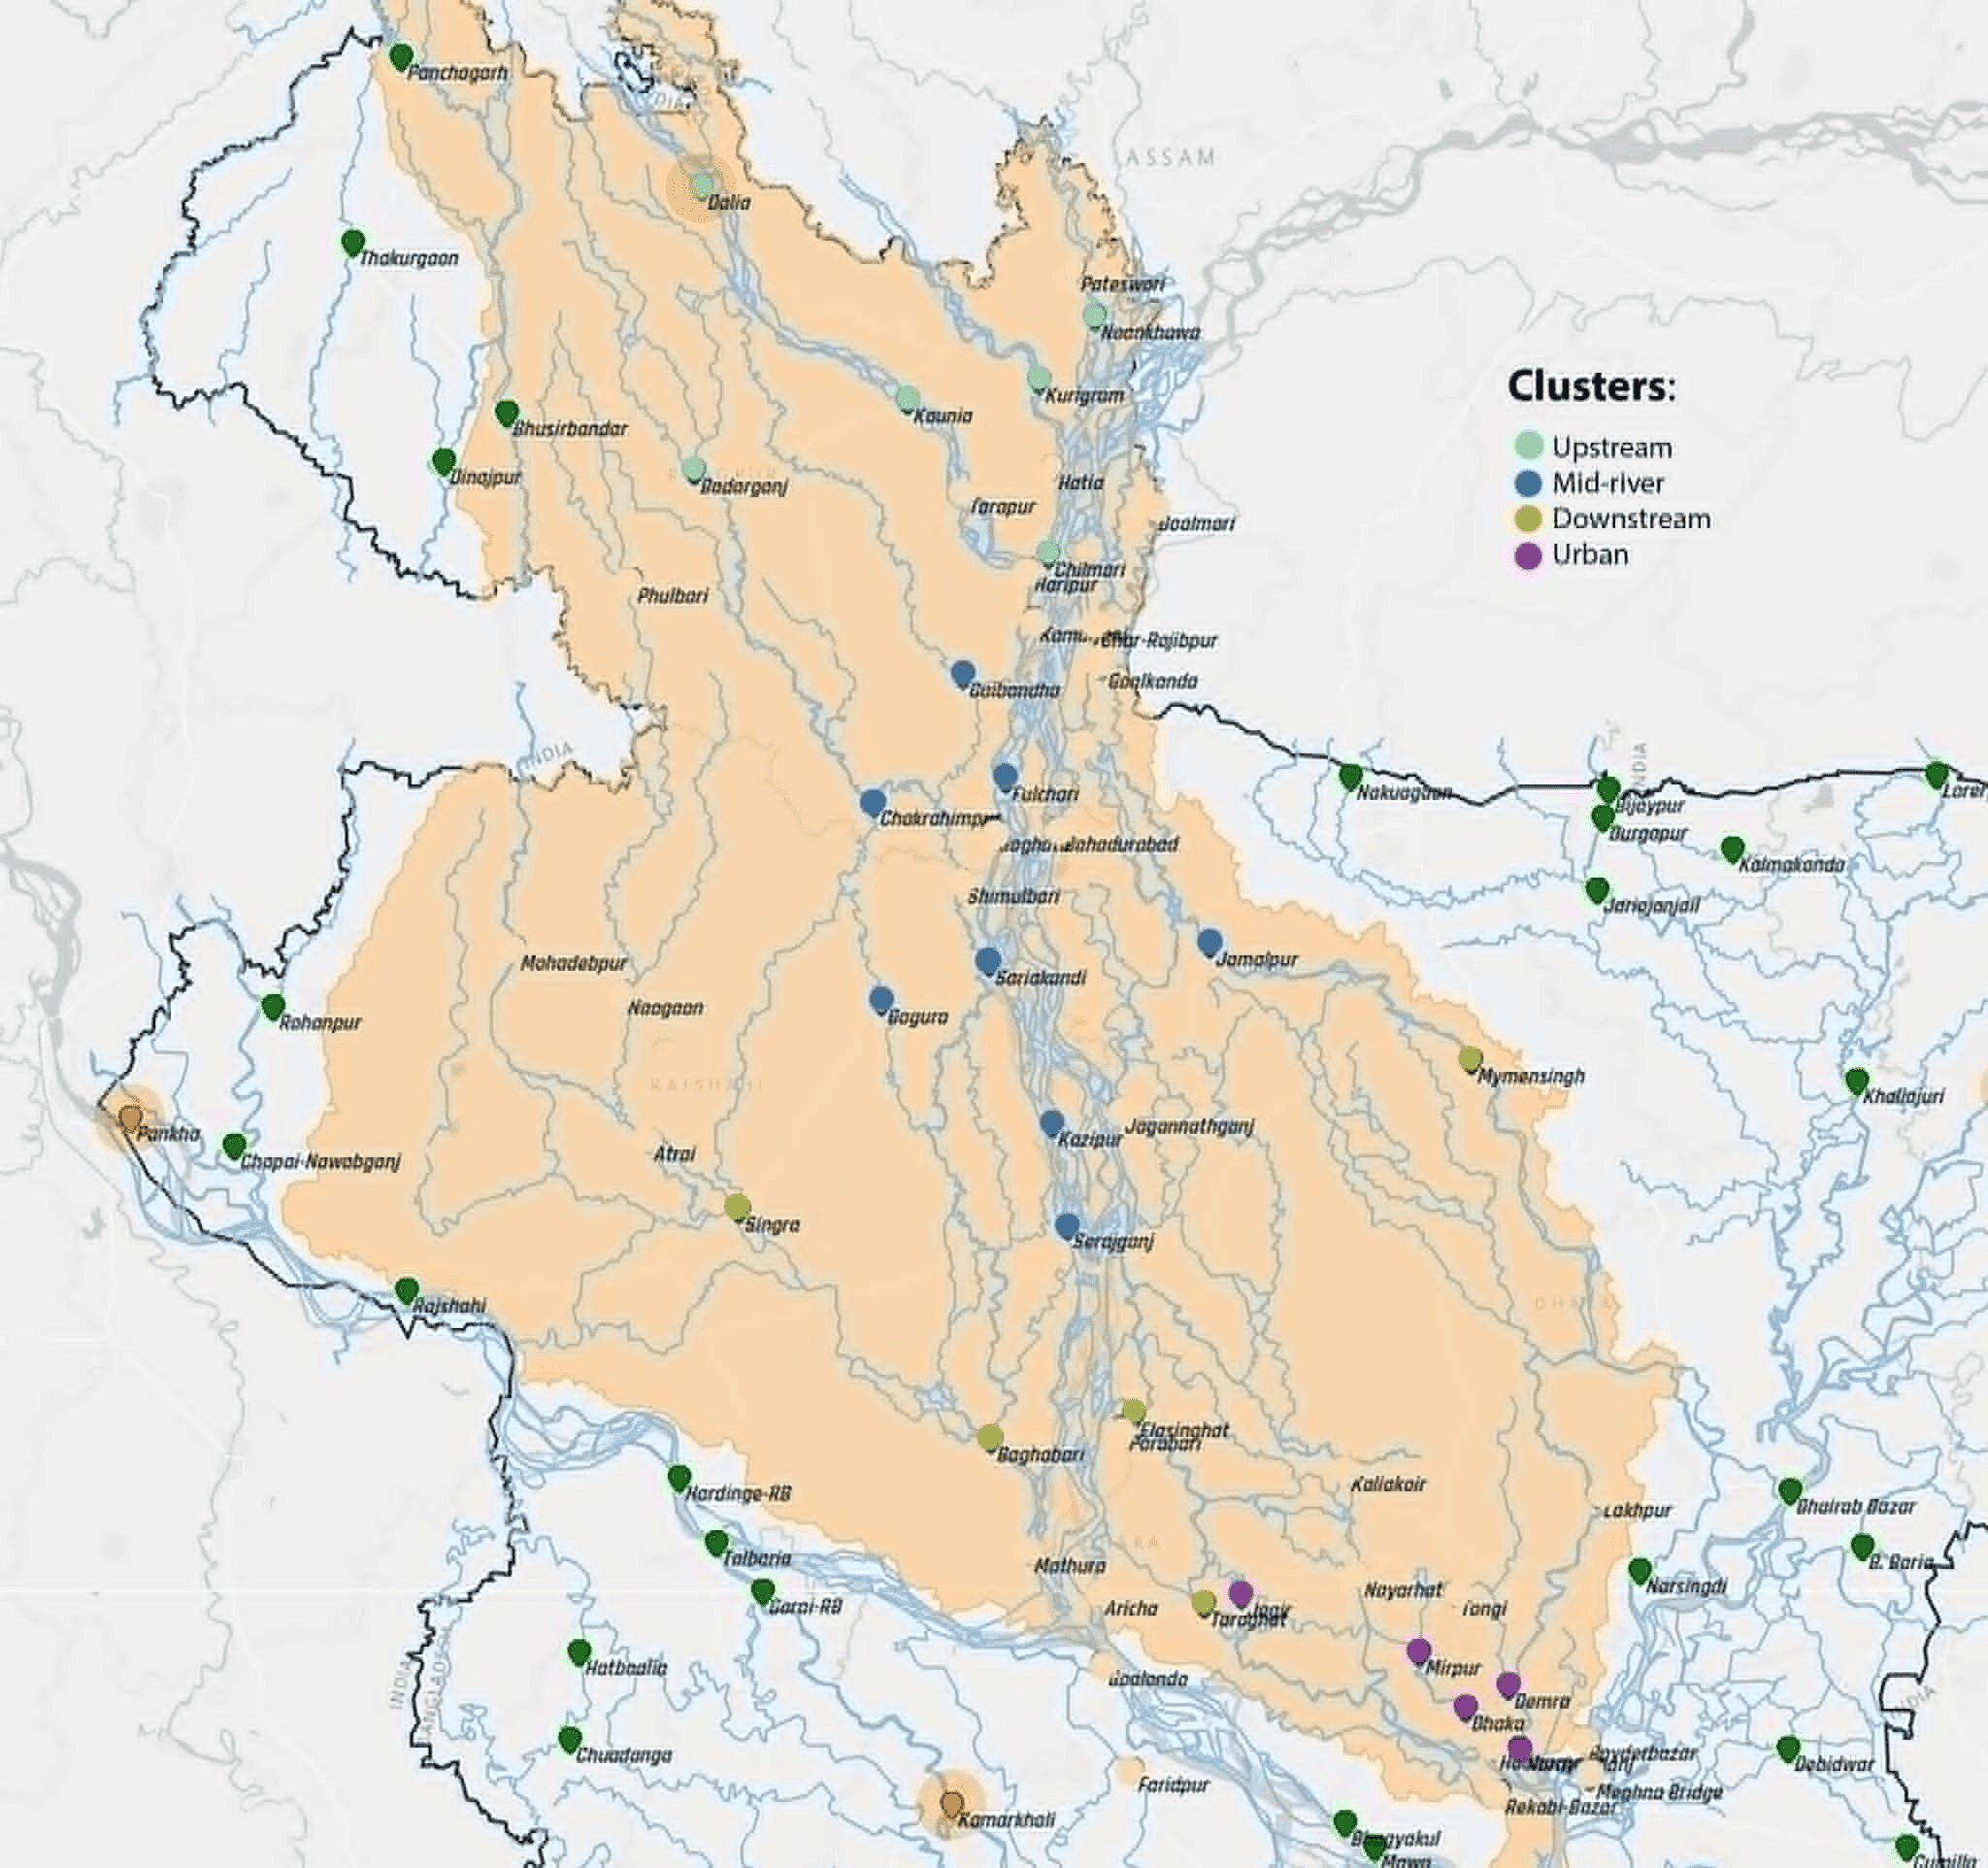
\includegraphics[
        width=0.8\textwidth
    ]{figures2/fig3-6a-cluster-distribution.png}

    \caption{Spatial distribution of the 26 monitoring stations by cluster.}
    \label{fig:3.6}
\end{figure}

\subsection{Cluster Formation and Characteristics}
\label{sec:3.10.2}
The monitoring stations are grouped into four clusters: Upstream, Mid-river, Downstream, and Urban, according to their hydrological and temporal characteristics. This grouping allows the federated learning framework to account for the differences in water-level and flow patterns across stations while learning from stations with similar behavior.

\begin{landscape}
\begin{table}[htbp]
  \centering
  \caption{Cluster Characteristics}
  \label{tab:3.5}
  \footnotesize
  \renewcommand{\arraystretch}{1.25}
  \begin{tabularx}{\linewidth}{@{}L{1.9cm} C{1.4cm} X X L{3.2cm}@{}}
    \toprule
    \textbf{Cluster} & \textbf{Stations} & \textbf{Rivers Represented} &
    \textbf{General Character} & \textbf{Representative Stations} \\
    \midrule
    Upstream & 6 & Teesta, Dharla, Deonai-Charalkata-Jamuneswari-Karatoa, Brahmaputra-Jamuna &
    Northernmost stations; non-tidal; closest to the point where flow enters Bangladesh from upstream catchments &
    Dalia, Kaunia, Kurigram \\

    Middle & 8 & Deonai-Charalkata-Jamuneswari-Karatoa, Ghagot, Brahmaputra-Jamuna, Old Brahmaputra &
    Central mainstem stations, largest cluster by station count; non-tidal &
    Bogra, Sirajganj, Jamalpur \\

    Downstream & 5 & Karatoa-Atrai-Gur-Gumani-Hurasagar, Old Brahmaputra, Dhaleswari, Kaliganga-Bethua &
    Distributary and secondary-channel reaches south of the main confluence zone; non-tidal &
    Baghabari, Mymensingh, Elashin \\

    Urban & 6 & Dhaleswari, Buriganga, Turag, Lakhya, Balu &
    Mostly Dhaka-metropolitan and tidally influenced (5 of 6 stations are Tidal-type --- the only Tidal stations in the dataset) &
    Dhaka (Mill Barrack), Mirpur, Narayanganj \\
    \bottomrule
  \end{tabularx}
\end{table}
\end{landscape}


% ------------------------------------------------------------
\section{Time-Series Input \& Forecasting Setup}
\label{sec:3.11}

Each model is trained on a sliding window of the past 30 days of daily observations across all five variables --- under the five-observations-per-day water-level schedule established in \S\ref{sec:3.9.3}, a 30-day input window corresponds to 150 water-level observations --- and asked to forecast water level at seven horizons: 3 hours, 6 hours, 12 hours, 1 day, 3 days, 7 days, and 15 days ahead, with the 15-day horizon corresponding to 75 water-level observations. Evaluating this wide a horizon range from a single 30-day input window is, as established in Chapter~2, wider than anything in the reviewed literature --- the closest precedents \cite{Kao2020,Cui2022} stop at 12 hours, and \cite{Islam2026a} reaches 30 days but only for discharge, at two stations, without any federated or clustered component.

\begin{figure}[htbp]
    \centering

    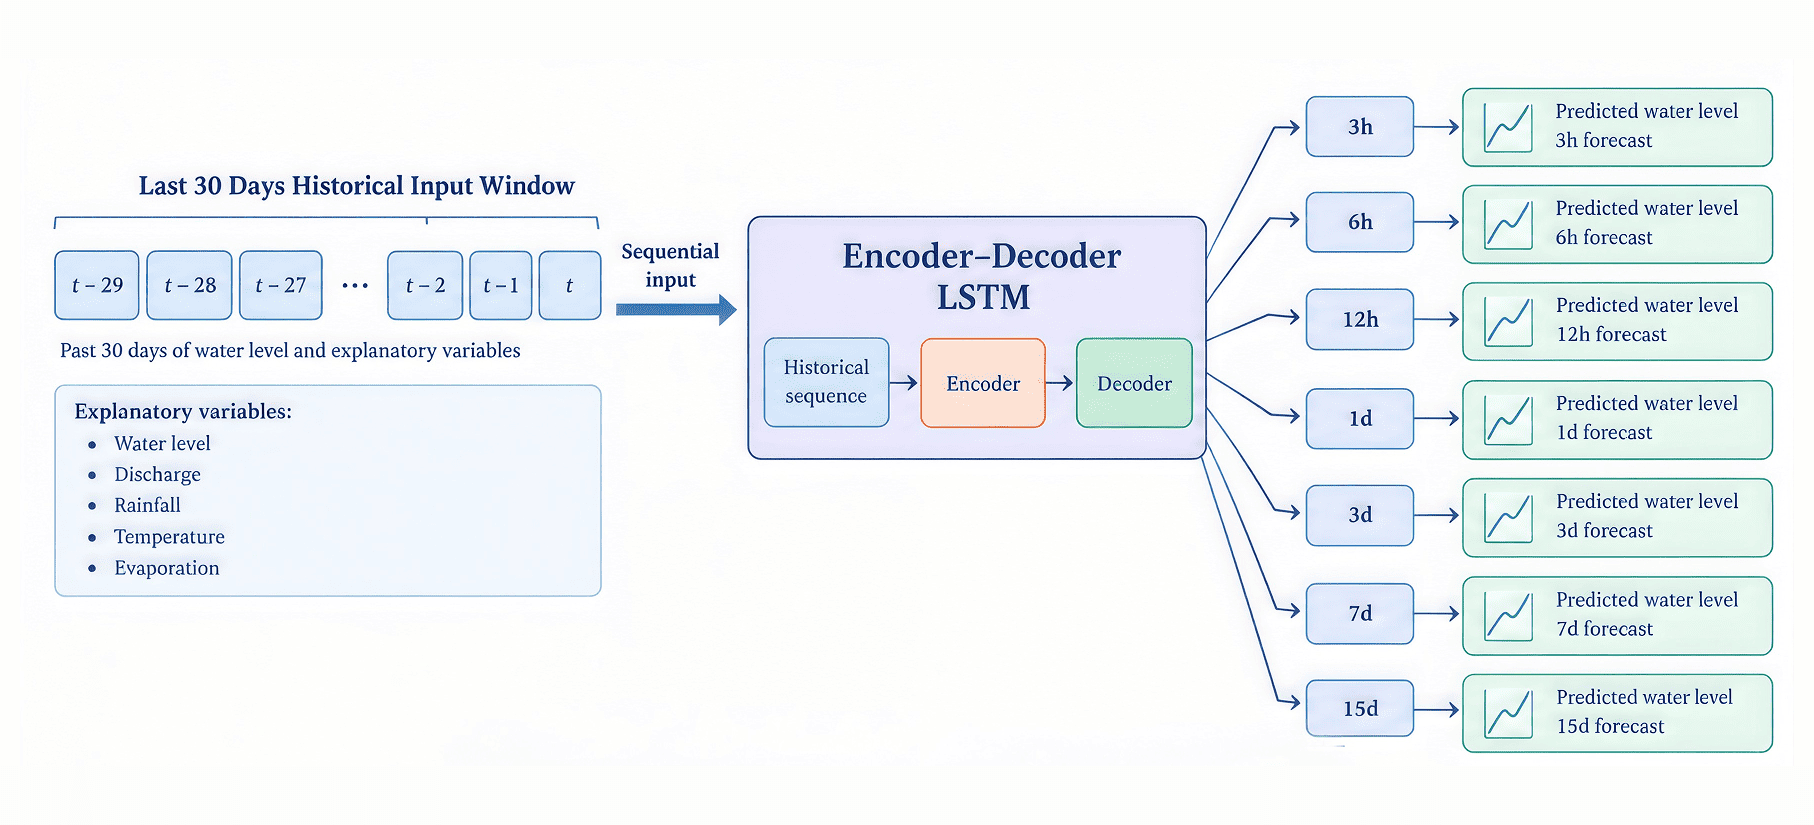
\includegraphics[
        width=0.9\textwidth
    ]{figures2/fig3-7-window-diagram.png}

    \caption{Time-series input/output window diagram.}
    \label{fig:3.7}
\end{figure}
% \chapter{Experimental Results and Analysis}
\label{Ch_Chapter5}

\section{Overview of Result Analysis }

This chapter presents the comprehensive results of the integrated multi-omics analysis for early versus late stage hepatocellular carcinoma (HCC) classification. The results include differential expression analysis, machine learning model performance, biomarker validation, and functional enrichment analysis, SHAP explainibility, molecular docking and drug discovery.


\section{Differential Expression Analysis}
\subsection{ Volcano Plot}

The volcano plot (Figure 4.1) displays the differential expression results for all 64,785 features comparing early stage (Stage I + II) versus late stage (Stage III + IV) HCC patients. The x-axis represents the log $ 2 $ fold change (Log $2$ FC), indicating the magnitude of expression difference between late and early stage. The y-axis represents the -log $ 10 $ (FDR), indicating the statistical significance of each feature.


\begin{figure}[H]
    \centering
    \includegraphics[width=.75\linewidth]{Figures/Figure1_Volcano_Plot.jpg}
    \caption{\textbf{Volcano Plot of Differential Multi-Omics Features}}
    \label{fig:Volcano Plot of Differential Multi-Omics}
\end{figure}

\begin{itemize}

    \item \textbf{Key Observations:}
    \begin{table}[htbp]
\centering
\caption{\textbf{Feature Categories from Differential Analysis}}
\label{tab:feature_categories}
\small
\begin{tabular}{|p{3.5cm}|c|p{2.5cm}|p{6cm}|}
\hline

\textbf{Category} & \textbf{Count} & \textbf{Color} & \textbf{Interpretation} \\
\hline
Not Significant & 64,653 & Gray & Features that did not meet significance thresholds \\
\hline
 Significant RNA & 130 & Red & RNA features with FDR < 0.05 and Log$_2$FC $>$ 0.5 \\
\hline
 Significant Methylation & 2 & Blue & CpG sites with FDR < 0.05 and Log$_2$FC $>$ 0.5 \\
\hline
\end{tabular}
\end{table}

    \item \textbf{Interpretation:}
    The volcano plot reveals a clear separation of significant features in the right and left tails of the distribution. The horizontal dashed line represents the FDR threshold of 0.05, while the vertical dashed lines represent the Log$_2$FC threshold of ±0.5. Features falling above the horizontal line and outside the vertical lines were considered significantly differentially expressed.

    \item \textbf{Biological Significance:} 
    The identification of 130 significant RNA features and 2 significant methylation features demonstrates that both transcriptional and epigenetic alterations contribute to HCC stage progression. The presence of features with extreme Log4FC values ( $>$ 0.5) suggests the involvement of key driver genes in the transition from early to late stage disease. 

\end{itemize}


\subsection{Top Differential Features Boxplots}

The boxplots (Figure 4.2) visualize the expression distribution of the top differential features across early and late stage patients.

\begin{figure}[!h]
    \centering
    \includegraphics[width=.8\linewidth]{Figures/Figure3_Boxplots.jpg}
    \caption{\textbf{Boxplots of Top Differential Features}}
    \label{fig:Boxplots of Top Differential Features}
\end{figure}

\begin{table}[htbp]
\centering
\caption{\textbf{Significant RNA Features from Differential Analysis}}
\label{tab:rna_features}
\small
\begin{tabular}{|l|c|c|l|}
\hline
\textbf{Feature} & \textbf{FDR} & \textbf{Log$_2$FC} & \textbf{Regulation} \\
\hline
ENSG00000223566.1 & 3.68e-02 & 0.029 & Up in Late Stage \\
\hline
ENSG00000268532.1 & 3.68e-02 & 0.005 & Up in Late Stage \\
\hline
\end{tabular}
\end{table}

The boxplots show that both RNA features exhibit slightly elevated expression in the late stage compared to early stage samples. The overlapping distributions indicate moderate effect sizes, which is consistent with the relatively small Log$_2$FC values (0.029 and 0.005).

\begin{table}[htbp]
\centering
\caption{\textbf{Significant Methylation Features from Differential Analysis}}
\label{tab:methylation_features}
\small
\begin{tabular}{|l|c|c|l|}
\hline
\textbf{Feature} & \textbf{FDR} & \textbf{Log$_2$FC} & \textbf{Regulation} \\
\hline
cg14619259 & 3.87e-02 & -0.207 & Down in Late Stage \\
\hline
cg07522644 & 4.45e-02 & -0.179 & Down in Late Stage \\
\hline
\end{tabular}
\end{table}

The methylation boxplots show decreased methylation (lower beta values) in the late stage compared to the early stage for both CpG sites. The beta values range from 0 to 1, with values closer to 0 indicating lower methylation. The observed down-regulation of methylation in the late stage suggests potential hypomethylation at these CpG sites, which could be associated with gene activation during cancer progression.\\

\textbf{Statistical Interpretation:} All four features showed statistically significant differences between early and late stage (FDR $<$ 0.05). The boxplots demonstrate that while the effect sizes are modest, the differences are consistent across patient samples, supporting their potential as stage-associated biomarkers.


\section{Machine Learning Model Performance}
\subsection{Cross-Validation Results}

\begin{figure}[H]
    \centering
    \includegraphics[width=.75\linewidth]{Figures/cross_validation_results_fixed.jpg}
    \caption{\textbf{5-Fold Cross-Validation Performance}}
    \label{fig:Cross-Validation}
\end{figure}

The cross-validation results (Figure 4.3) show the performance of all four models using 5-fold cross-validation. The Voting Ensemble achieved the highest cross-validated accuracy of 0.924, followed by SVM Linear (0.901), XGBoost (0.881), and Random Forest (0.864).

\begin{table}[htbp]
\centering
\caption{\textbf{Cross-Validated Accuracy of Machine Learning Models}}
\label{tab:cv_accuracy}
\small
\begin{tabular}{|l|c|}
\hline
\textbf{Model} & \textbf{Cross-Validated Accuracy} \\
\hline
Voting Ensemble & 0.924 \\
\hline
SVM Linear & 0.901 \\
\hline
XGBoost & 0.881 \\
\hline
Random Forest & 0.864 \\
\hline
Random Classifier & 0.500 \\
\hline
\end{tabular}
\end{table}

\textbf{Interpretation: }The Voting Ensemble model outperformed all individual models, demonstrating the benefit of combining multiple algorithms through soft voting. The ensemble approach leverages the complementary strengths of SVM, Random Forest, and XGBoost, reducing individual model biases and improving overall prediction accuracy. The consistent performance across all folds (as indicated by the error bars) suggests that the model is robust and generalizable.

\subsection{Confusion Matrix}

\begin{figure}[H]
    \centering
    \includegraphics[width=.75\linewidth]{Figures/confusion_matrices_all_models_fix.jpg}
    \caption{\textbf{Confusion Matrices for All Models} }
    \label{Confusion Matrices}
\end{figure}

The confusion matrices (Figure 4.4) provide a detailed breakdown of classification performance for each model.\\
\textbf{SVM Linear:}\\
True Positives (Late correctly predicted): 8\\
True Negatives (Early correctly predicted): 32\\
False Positives (Early incorrectly predicted as Late): 6\\
False Negatives (Late incorrectly predicted as Early): 4\\ \\
\textbf{Random Forest:}\\
True Positives(Late correctly predicted): 5\\
True Negatives(Early correctly predicted): 33\\
False Positives(Early incorrectly predicted as Late): 5\\
False Negatives(Late incorrectly predicted as Early): 7\\
\textbf{XGBoost:}\\
True Positives(Late correctly predicted): 7\\
True Negatives(Early correctly predicted): 32\\
False Positives(Early incorrectly predicted as Late): 6\\
False Negatives(Late incorrectly predicted as Early): 5\\
\textbf{Ensemble Soft Voting:}\\
True Positives(Late correctly predicted): 8\\
True Negatives(Early correctly predicted): 33\\
False Positives(Early incorrectly predicted as Late): 5\\
False Negatives(Late incorrectly predicted as Early): 4\\\\
\textbf{Interpretation:} The confusion matrices demonstrate that the Voting Ensemble model achieved the highest accuracy with the fewest misclassifications. The balanced performance across both early and late stage classes indicates that the models are not biased toward the majority class (early stage).


\subsection{ROC Curves}

\begin{figure}[H]
    \centering
    \includegraphics[width=.8\linewidth]{Figures/roc_curves_all_models.jpg}
    \caption{\textbf{ROC Curve of all Models}}
    \label{fig:ROC Curve}
\end{figure}

 The Receiver Operating Characteristic (ROC) curves were generated to evaluate and compare the discriminatory ability of all four machine learning models. The ROC curve plots the True Positive Rate (Sensitivity) against the False Positive Rate (1 - Specificity) across all possible classification thresholds, providing a comprehensive measure of model performance independent of any single threshold.\\
\textbf{Interpretation:}
The ROC curves demonstrate that SVM Linear achieved the highest AUC of 0.844, indicating excellent discriminatory ability between early and late stage HCC. The Voting Ensemble (AUC = 0.825) and XGBoost (AUC = 0.796) also showed good performance, while Random Forest (AUC = 0.787) showed fair discrimination.\\
\textbf{Clinical Interpretation:} An AUC of 0.844 indicates that there is an 84.4 percent chance that a randomly selected late stage patient will have a higher predicted probability of late stage disease than a randomly selected early stage patient. This level of discrimination is considered clinically useful for stage prediction.

\begin{table}[htbp]
\centering
\caption{\textbf{Comparison of Model Performance by AUC}}
\label{tab:auc_comparison}
\small
\begin{tabular}{|l|c|l|}
\hline
\textbf{Model} & \textbf{AUC} & \textbf{Rank} \\
\hline
SVM Linear & 0.844 & 1st (Best) \\
\hline
Voting Ensemble & 0.825 & 2nd \\
\hline
XGBoost & 0.796 & 3rd \\
\hline
Random Forest & 0.787 & 4th \\
\hline
\end{tabular}
\end{table}

\textbf{Performance at Optimal Threshold:}\\
The ROC curves reveal that all models achieve high sensitivity and specificity at intermediate thresholds. The SVM Linear model shows the most favorable trade-off between sensitivity and specificity, with the curve closest to the top-left corner of the plot.

\textbf{Clinical Relevance:}\\
The high AUC values demonstrate that the models can effectively separate early from late stage patients. This is clinically significant because accurate stage classification is essential for:
\begin{itemize}
    \item \textbf{Treatment Selection:} Early stage patients may receive curative treatments (surgery, ablation), while late stage patients receive systemic therapy.
    \item \textbf{Prognosis:} Early stage patients have 60-70 percent  5-year survival, while late stage patients have only 10-20 percent.

    \item \textbf{Patient Management:} Accurate classification guides clinical decision-making and resource allocation.
\end{itemize}

\subsection{Comparison of Machine Learning Model Performance}
\begin{table}[htbp]
\centering
\caption{\textbf{Comparison of machine learning models and ensemble approaches}}
\label{tab:model_comparison}
\resizebox{\textwidth}{!}{%
\begin{tabular}{lcccccccc}
\toprule
\textbf{Model} & \textbf{Train (s)} & \textbf{Predict (s)} & 
\textbf{Total (s)} & \textbf{Bal. Acc.} & \textbf{Precision} & 
\textbf{Recall} & \textbf{F1} & \textbf{AUC} \\
\midrule
Linear SVM & 0.0247 & 0.0015 & 0.0262 & 0.7281 & 0.5000 & 0.6667 & 0.5714 & 0.8443 \\
Random Forest & 0.1511 & 0.0346 & 0.1858 & 0.6689 & 0.6250 & 0.4167 & 0.5000 & 0.7873 \\
XGBoost & 0.1902 & 0.0015 & 0.1917 & 0.7127 & 0.5385 & 0.5833 & 0.5600 & 0.7961 \\
3-Model Soft Voting & 0.3337 & 0.0359 & 0.3695 & 0.7412 & 0.5333 & 0.6667 & 0.5926 & 0.8246 \\
2-Model SVM+XGB & 0.2034 & 0.0032 & 0.2066 & 0.7281 & 0.5000 & 0.6667 & 0.5714 & 0.8268 \\
\bottomrule
\end{tabular}%
}
\end{table}


Table 4.6 presents a comparative evaluation of the individual machine learning models and ensemble approaches based on training time, prediction time, total computational time, balanced accuracy, precision, recall, F1-score, and ROC-AUC.

\textbf{The Linear SVM} achieved a balanced accuracy of \textbf{72.81\%}, with a precision of 50.00\%, recall of 66.67\%, and F1-score of 57.14\%. It also obtained the highest ROC-AUC value of 0.8443 among all the evaluated models, indicating good discrimination between the early-stage and advanced-stage classes. In addition, the Linear SVM required the lowest total computational time, with a total execution time of only \textbf{0.0262 seconds.}\\

\textbf{The Random Forest model} produced a balanced accuracy of \textbf{66.89\%,} which was the lowest among the evaluated models. It achieved a precision of 62.50\%, recall of 41.67\%, and F1-score of 50.00\%, with an ROC-AUC of 0.7873. Although Random Forest showed the highest precision among the individual models, its relatively lower recall indicates that it identified a smaller proportion of the positive-class samples.\\

\textbf{The XGBoost model} achieved a balanced accuracy of \textbf{71.27\%}, with a precision of 53.85\%, recall of 58.33\%, and F1-score of 56.00\%. The model obtained an ROC-AUC of 0.7961. Its total computational time was \textbf{0.1917 seconds}, which was higher than that of the Linear SVM but comparable to the Random Forest model.\\

\textbf{The three-model soft voting ensemble}, which combined Linear SVM, Random Forest, and XGBoost, achieved the highest balanced accuracy of \textbf{74.12\%} among all the evaluated approaches. The ensemble also obtained a recall of 66.67\% and an F1-score of 59.26\%, with an ROC-AUC of 0.8246. Although its ROC-AUC was slightly lower than that of the Linear SVM, the three-model ensemble provided the highest balanced accuracy, suggesting that combining the predictions of the three classifiers improved the balance of classification performance between the two disease-stage classes. However, this improvement was associated with a higher computational cost, with a total execution time of \textbf{0.3695 seconds.}\\

\textbf{The two-model soft voting ensemble} combining Linear SVM and XGBoost achieved a balanced accuracy of \textbf{72.81\%}, with a precision of 50.00\%, recall of 66.67\%, and F1-score of 57.14\%. The ROC-AUC of this ensemble was 0.8268, which was higher than the ROC-AUC obtained by XGBoost and the three-model soft voting ensemble, although it remained lower than that of the Linear SVM. The total computational time was \textbf{0.2066 seconds}, making this approach considerably faster than the three-model ensemble.\\

Overall, the three-model soft voting ensemble demonstrated the highest balanced accuracy, achieving 74.12\%. In contrast, the Linear SVM achieved the highest ROC-AUC of 0.8443 and required the lowest computational time. The Random Forest model obtained the highest precision among the individual classifiers, while the Linear SVM, three-model soft voting ensemble, and two-model SVM--XGBoost ensemble achieved the highest recall of 66.67\%. Therefore, the results indicate that the three-model soft voting approach provided the best performance when balanced accuracy was considered as the primary evaluation criterion, whereas \textbf{Linear SVM }demonstrated stronger discrimination and computational efficiency based on ROC-AUC and execution time.

\section{Feature Importance Analysis}
\subsection{Top 20 Feature Importance}

\begin{figure}[H]
    \centering
    \includegraphics[width=.80\linewidth]{Figures/top20_feature_importance.jpg}
    \caption{\textbf{Top 20 Features for Stage Prediction}}
    \label{fig:Top 20 Features}
\end{figure}

The feature importance plot (Figure 4.6) displays the top 20 features ranked by their contribution to the Random Forest model. The top features include:
\textbf{Interpretation:} The feature importance analysis reveals that ENSG00000223566.1 is the most important feature for stage prediction, with an importance score of 0.045. The top 20 features collectively contribute approximately 0.300 to the model's predictive power. The gradual decline in importance scores suggests that a moderate number of features (20-50) is sufficient for accurate classification, supporting our feature selection strategy.\\
\textbf{Biological Relevance:} The identified top features include genes involved in various cancer-related pathways, including cell cycle regulation, signal transduction, and metabolic processes. The presence of both RNA and methylation features in the top 20 list highlights the complementary value of multi-omics data for cancer stage prediction.

\subsection{Heatmap of Top 30 Differential Features}

\begin{figure}[H]
    \centering
    \includegraphics[width=.75\linewidth]{Figures/Figure2_Heatmap.jpg}
    \caption{\textbf{Heatmap of Top 30 Differential Features}}
    \label{fig:Top 30 Differential Features}
\end{figure}
The heatmap (Figure 4.7) visualizes the expression patterns of the top 30 differential features across all patients. Each row represents a feature and each column represents a patient. The color gradient represents the Z-score, with red indicating higher expression and blue indicating lower expression.
\begin{table}[htbp]
\centering
\caption{\textbf{Feature Group Observations from Differential Analysis}}
\label{tab:feature_observations}
\small
\begin{tabular}{|p{4cm}|p{10cm}|}
\hline
\textbf{Feature Group} & \textbf{Observation} \\
\hline
Upregulated Features & Genes with increased expression in late stage patients \\
\hline
Downregulated Features & Genes with decreased expression in late stage patients \\
\hline
Methylation Features & CpG sites with altered methylation patterns \\
\hline
\end{tabular}
\end{table}
\textbf{Interpretation:} The heatmap reveals distinct clustering patterns between early and late stage patients. Late stage patients show a characteristic expression signature with multiple features consistently upregulated or downregulated. This clustering pattern suggests that the top 30 features collectively capture a biological signature associated with stage progression.

\section{Validated Biomarkers}
\subsection{ Volcano Plot with Validated Biomarkers}
\begin{figure}[H]
    \centering
    \includegraphics[width=.75\linewidth]{Figures/volcano_plot_fixed.jpg}
    \caption{\textbf{Volcano Plot Highlighting Validated Biomarkers}}
    \label{fig:Volcano Plot}
\end{figure}

The volcano plot with validated biomarkers shows the position of the 8 validated genes relative to the differential expression thresholds.
\begin{table}[htbp]
\centering
\caption{\textbf{Validated Biomarkers from SHAP Analysis and GEO Validation}}
\label{tab:validated_biomarkers from SHAP Analysis and GEO Validation}
\small
\begin{tabular}{|l|c|c|l|c|}
\hline
\textbf{Gene} & \textbf{Log$_2$FC} & \textbf{FDR} & \textbf{Regulation} & \textbf{Validation Status} \\
\hline
CCL16 & -1.022 & 0.00113 & Down & $\checkmark$ Validated \\
\hline
PCCB & -0.632 & 0.00042 & Down & $\checkmark$ Validated \\
\hline
ATOX1 & -0.601 & 0.00036 & Down & $\checkmark$ Validated \\
\hline
ECT2 & 0.557 & 0.04476 & Up & $\checkmark$ Validated \\
\hline
BICD2 & 0.440 & 0.00042 & Up & $\checkmark$ Validated \\
\hline
EIF4E & 0.408 & 0.00054 & Up & $\checkmark$ Validated \\
\hline
VEGFA & 0.362 & 0.04476 & Up & $\checkmark$ Validated \\
\hline
ANGPT2 & 0.236 & 0.00293 & Up & $\checkmark$ Validated \\
\hline
\end{tabular}
\end{table}
\\
\textbf{Interpretation:} The 8 validated biomarkers are clearly visible in the volcano plot. CCL16 shows the most extreme Log $ 2 $ FC (-1.022), indicating strong down-regulation in the late stage. ECT2 and VEGFA show Log $ 2 $ FC values above the 0.5 threshold, while BICD2, EIF4E, and ANGPT2 show moderate Log $ 2 $ FC values (0.23-0.44) that still achieve statistical significance.

\textbf{Biological Significance:} The validation of these 8 genes on independent GEO data confirms their robustness as stage-specific biomarkers. The mix of upregulated and downregulated genes reflects the complex molecular changes occurring during cancer progression.

\section{Functional Enrichment Analysis}
\subsection{GO Biological Process Network}
\begin{figure}[H]
    \centering
    \includegraphics[width=.75\linewidth]{Figures/network.jpg}
    \caption{\textbf{GO Biological Process Network for Validated Biomarkers}}
    \label{fig:GO Biological}
\end{figure}
The network diagram  visualizes the Gene Ontology (GO) biological processes associated with the validated biomarkers.
\begin{table}[htbp]
\centering
\caption{\textbf{Gene Ontology (GO) Enrichment Analysis of Validated Biomarkers}}
\label{tab:go_enrichment}
\small
\begin{tabular}{|p{5.5cm}|p{3cm}|p{4.5cm}|}
\hline
\textbf{GO Term} & \textbf{Genes Involved} & \textbf{Biological Process} \\
\hline
Activation of protein kinase activity (GO:0032147) & VEGFA, ECT2 & Signal transduction \\
\hline
Regulation of blood vessel endothelial cell migration (GO:0043535) & VEGFA, ANGPT2 & Angiogenesis \\
\hline
Regulation of positive chemotaxis (GO:0050926) & VEGFA & Cell migration \\
\hline
Positive regulation of hydrolase activity (GO:0051345) & VEGFA & Enzyme regulation \\
\hline
Positive regulation of protein kinase activity (GO:0045860) & VEGFA, ECT2 & Signal transduction \\
\hline
\end{tabular}
\end{table}
\\
\textbf{Interpretation:} The GO network reveals that the validated biomarkers are primarily involved in angiogenesis (VEGFA, ANGPT2), cell cycle regulation (ECT2), and signal transduction (VEGFA, ECT2). These processes are well-established hallmarks of cancer progression.

\subsection{ KEGG Pathway Network}
\begin{figure}[H]
    \centering
    \includegraphics[width=.70\linewidth]{Figures/network (1).jpg}
    \caption{\textbf{ KEGG Pathway Network for Validated Biomarkers}}
    \label{fig:KEGG Pathway}
\end{figure}
The KEGG pathway network (Figure 4.10) shows the signaling pathways enriched among the validated biomarkers.
\begin{table}[htbp]
\centering
\caption{\textbf{Pathway Enrichment Analysis of Validated Biomarkers}}
\label{tab:pathway_enrichment}
\small
\begin{tabular}{|p{4.5cm}|p{3.5cm}|p{5.5cm}|}
\hline
\textbf{Pathway} & \textbf{Genes Involved} & \textbf{Biological Relevance} \\
\hline
Ras signaling pathway & VEGFA & Cell proliferation \\
\hline
Rap1 signaling pathway & ANGPT2 & Cell adhesion, migration \\
\hline
PI3K-Akt signaling pathway & VEGFA & Cell survival, angiogenesis \\
\hline
HIF-1 signaling pathway & VEGFA & Response to hypoxia \\
\hline
Kaposi sarcoma-associated herpesvirus infection & VEGFA & Viral oncogenesis \\
\hline
\end{tabular}
\end{table}
\\
\textbf{Interpretation:} The KEGG pathway analysis confirms that the validated biomarkers are involved in key cancer-related pathways. The PI3K-Akt and HIF-1 signaling pathways are particularly relevant to HCC progression, as they regulate cell survival, angiogenesis, and response to hypoxia.

\section{SHAP Explainability Analysis}
\subsection{SHAP Analysis of the 132 Selected Biomarkers}
To investigate the contribution of all selected biomarkers, Also performed SHAP analysis using the complete set of 132 important genes obtained after feature selection.\\
The SHAP feature importance plot shown in Figure 4.11 ranks the twenty most influential biomarkers based on their mean absolute SHAP values. Among all genes, TNRC18P2 exhibited the highest SHAP importance score, indicating that it contributed the most to the prediction of HCC progression. 

\begin{figure}[H]
    \centering
    \includegraphics[width=.75\linewidth]{Figures/SHAP_Bar_GeneNames.jpg}
    \caption{\textbf{The SHAP feature importance plot}}
    \label{fig:SHAP feature}
\end{figure}

Several additional genes, including RPL5P4, FAM163A, ENSG00000287528, SCTR, WBP11P3, EPYC, LAMTOR3, PCCB, SPANXC, and SPANXA2-OT1, also demonstrated relatively high importance. Interestingly, although PCCB was ranked lower than TNRC18P2 in the complete biomarker analysis, it remained among the most influential genes and was later validated using the external GEO dataset.\\


\begin{figure}[H]
    \centering
    \includegraphics[width=.75\linewidth]{Figures/SHAP_Summary_GeneNames.jpg}
    \caption{\textbf{SHAP summary plot}}
    \label{fig:SHAP summary}
\end{figure}

The SHAP summary plot presented in Figure 4.12 illustrates both the importance and direction of feature contributions across all patient samples. Each point represents an individual sample, and the color indicates the corresponding gene expression level. The wide spread of SHAP values observed for TNRC18P2 confirms its strong influence on the model prediction. Similarly, genes such as RPL5P4, FAM163A, SCTR, and PCCB also showed noticeable impacts, although their contributions were smaller than that of TNRC18P2. The summary plot also demonstrates that different expression levels can either increase or decrease the predicted probability depending on the patient, highlighting the complex relationships captured by the machine learning model.\\

\begin{figure}[H]
    \centering
    \includegraphics[width=.85\linewidth]{Figures/SHAP_Waterfall.jpg}
    \caption{\textbf{SHAP waterfall plot}}
    \label{fig:SHAP waterfall}
\end{figure}
Figure 4.13 presents the SHAP waterfall plot for one representative prediction using the complete biomarker set. The waterfall plot shows how individual genes collectively influenced the model output. Among all biomarkers, RPL5P4, cg14619259, TNRC18P2, ENSG00000287528, PCCB, and cg07522644 produced the largest negative SHAP contributions, while FAM163A provided the largest positive contribution. The remaining biomarkers had comparatively smaller effects on the final prediction. This visualization demonstrates how multiple genes interact to produce the final classification rather than relying on a single biomarker alone.

\subsection{SHAP Analysis of the Eight Validated Biomarkers}

\begin{figure}[H]
    \centering
    \includegraphics[width=.85\linewidth]{Figures/SHAP_8_Biomarkers_Bar.jpg}
    \caption{\textbf{The SHAP 8 biomarkers importance plot}}
    \label{fig:SHAP 8 biomarkers}
\end{figure}
Figure 4.14 presents the SHAP feature importance plot for the eight validated biomarkers. The results clearly indicate that PCCB had the highest average SHAP value among all validated genes, demonstrating that it contributed the most to the prediction of HCC stage. The remaining biomarkers, including ANGPT2, VEGFA, ATOX1, BICD2, ECT2, EIF4E, and CCL16, showed comparatively lower contributions. Although these genes influenced the model prediction, their impact was considerably smaller than that of PCCB. Based on this finding, considered PCCB to be the most influential validated biomarker and selected it for further molecular docking and drug discovery analysis.\\

\begin{figure}[H]
    \centering
    \includegraphics[width=.75\linewidth]{Figures/SHAP_Summary_GeneNames.jpg}
    \caption{\textbf{SHAP 8 biomarker summary plot}}
    \label{fig:SHAP 8 biomarker summary plot}
\end{figure}
The SHAP summary plot shown in Figure 4.15 provides additional insight into how each biomarker influenced the model. Each point represents one patient sample, while the color indicates the gene expression level. Red points correspond to higher expression values, whereas blue points indicate lower expression values. PCCB displayed the widest distribution of SHAP values, confirming that variations in its expression produced the greatest influence on model predictions. The remaining biomarkers exhibited relatively narrow SHAP distributions, suggesting a more moderate effect on classification performance.\\

\begin{figure}[H]
    \centering
    \includegraphics[width=.8\linewidth]{Figures/SHAP_Waterfall.jpg}
    \caption{\textbf{SHAP 8 biomarker waterfall plot}}
    \label{fig:8 biomarker waterfall}
\end{figure}
To further explain the contribution of individual biomarkers for a representative prediction, generated the SHAP waterfall plot shown in Figure 4.16. This figure illustrates how each validated biomarker contributed to the final prediction for a single patient. Among all biomarkers, PCCB produced the largest SHAP contribution, indicating that it was the primary factor influencing the model output. The remaining genes, including ATOX1, VEGFA, ANGPT2, ECT2, BICD2, EIF4E, and CCL16, showed comparatively smaller positive or negative contributions. This result further confirms the dominant role of PCCB in distinguishing between early- and late-stage HCC patients.\\

Overall, the SHAP analysis consistently demonstrated that \textbf{PCCB is the most important validated} biomarker in my predictive model. Therefore, PCCB is selected as the primary target for subsequent protein structure analysis, molecular docking, and drug discovery.\\

Overall, the SHAP analysis of the complete biomarker set identified \textbf{TNRC18P2} as the most influential biomarker within the machine learning model. However, after external validation using the independent GEO dataset, \textbf{PCCB }emerged as the most reliable and biologically validated biomarker. Therefore, PCCB was selected for downstream molecular docking, drug screening, and therapeutic candidate identification because it demonstrated both strong predictive capability and successful external validation.

\section{Molecular Docking Analysis for RNA Features}
 \subsection{Docking Against PCCB}
 
\subsubsection{Target Protein and Binding Site Identification}

Three-dimensional structure of PCCB (Propionyl-CoA Carboxylase Beta subunit) is obtained from the Protein Data Bank under the accession code 8ZUX. This structure was determined using electron microscopy at a resolution of 2.68 Å and contains the PCCB protein with its natural cofactors, including ATP, Biotin, and Magnesium.Protein structure is prepared for docking by removing water molecules and adding hydrogen atoms.The C2 pocket is identified as the primary binding site based on its location near the ATP-binding region, where natural ligands are positioned. This findings selected this pocket as the target for all docking simulations.

\subsubsection{Molecular Docking of Sorafenib}

Molecular docking of Sorafenib against PCCB using CB-Dock2, and the results are preented in Table 4.11. The docking analysis revealed that Sorafenib bound most favorably to the C2 pocket, achieving a Vina score of -10.0 kcal/mol. This pocket had a cavity volume of 1119 ų and was centered at coordinates 170, 134, 200. This set the docking grid to 27 × 27 × 27 Å, ensuring comprehensive coverage of the binding site.

\begin{table}[htbp]
\centering
\caption{\textbf{Molecular Docking Results of Sorafenib Against PCCB}}
\label{tab:sorafenib_docking}
\small
\begin{tabular}{|p{1.5cm}|p{2.0cm}|p{1.5cm}|p{2.5cm}|p{2.5cm}|}
\hline
\textbf{Pocket ID} & \textbf{Vina Score (kcal/mol)} & \textbf{Cavity Volume (\AA³)} & \textbf{Center (x, y, z)} & \textbf{Docking Size (x, y, z)} \\
\hline
C2 & -10.0 & 1119 & 170, 134, 200 & 27, 27, 27 \\
\hline
C3 & -9.2 & 699 & 163, 138, 192 & 27, 27, 27 \\
\hline
C4 & -9.2 & 605 & 188, 122, 160 & 27, 27, 27 \\
\hline
C1 & -8.9 & 4746 & 186, 111, 209 & 35, 35, 35 \\
\hline
C5 & -6.9 & 347 & 165, 143, 150 & 27, 27, 27 \\
\hline
\end{tabular}
\end{table}

Sorafenib showed promising binding to other pockets, including C3 (-9.2 kcal/mol, volume 699 ų), C4 (-9.2 kcal/mol, volume 605 ų), C1 (-8.9 kcal/mol, volume 4746 ų), and C5 (-6.9 kcal/mol, volume 347 ų). Consistently found that the strongest binding was at the C2 pocket, suggesting this is the preferred binding site for Sorafenib on PCCB.

\subsubsection{Molecular Docking of Regorafenib}

The docking results are represented for Regorafenib in Table 4.12. Similar to Sorafenib, found that Regorafenib exhibited the strongest binding affinity at the C2 pocket, with a Vina score of -9.6 kcal/mol. The C2 pocket maintained the same cavity volume of 1119 ų and center coordinates of 170, 134, 200, with a slightly reduced docking size of 23 × 23 × 23 Å compared to Sorafenib.\\
\begin{table}[htbp]
\centering
\caption{\textbf{Molecular Docking Results of Regorafenib Against PCCB}}
\label{tab:regorafenib_docking}
\small
\begin{tabular}{|p{1.5cm}|p{2.0cm}|p{1.5cm}|p{2.5cm}|p{2.5cm}|}
\hline
\textbf{Pocket ID} & \textbf{Vina Score (kcal/mol)} & \textbf{Cavity Volume (\AA³)} & \textbf{Center (x, y, z)} & \textbf{Docking Size (x, y, z)} \\
\hline
C2 & -9.6 & 1119 & 170, 134, 200 & 23, 23, 23 \\
\hline
C1 & -9.5 & 4746 & 186, 111, 209 & 35, 35, 35 \\
\hline
C4 & -8.1 & 605 & 188, 122, 160 & 23, 23, 23 \\
\hline
C3 & -8.0 & 699 & 163, 138, 192 & 23, 23, 23 \\
\hline
C5 & -7.3 & 347 & 165, 143, 150 & 23, 23, 23 \\
\hline
\end{tabular}
\end{table}
Regorafenib demonstrated favorable binding to the C1 pocket (-9.5 kcal/mol, volume 4746 ų), C4 pocket (-8.1 kcal/mol, volume 605 ų), C3 pocket (-8.0 kcal/mol, volume 699 ų), and C5 pocket (-7.3 kcal/mol, volume 347 ų). This process noted that the consistent preference for the C2 pocket across both Sorafenib and Regorafenib suggests that this binding site is structurally favorable for kinase inhibitors targeting PCCB.

\subsubsection{Molecular Docking of Cabozantinib}

Cabozantinib demonstrated the most promising binding affinity among all tested drugs, achieving a Vina score of -10.8 kcal/mol at the C2 pocket, as shown in Table 4.13. This was the highest binding affinity across all docking simulations, indicating the strongest predicted interaction with PCCB. The C2 pocket maintained its consistent characteristics with a volume of 1119 ų and center at 170, 134, 200, with a docking size of 25 × 25 × 25 Å.\\
\begin{table}[htbp]
\centering
\caption{\textbf{Molecular Docking Results of Cabozantinib Against PCCB}}
\label{tab:cabozantinib_docking}
\small
\begin{tabular}{|p{1.5cm}|p{2.0cm}|p{1.5cm}|p{2.5cm}|p{2.5cm}|}
\hline
\textbf{Pocket ID} & \textbf{Vina Score (kcal/mol)} & \textbf{Cavity Volume (\AA³)} & \textbf{Center (x, y, z)} & \textbf{Docking Size (x, y, z)} \\
\hline
C2 & -10.8 & 1119 & 170, 134, 200 & 25, 25, 25 \\
\hline
C1 & -9.4 & 4746 & 186, 111, 209 & 35, 35, 35 \\
\hline
C3 & -9.0 & 699 & 163, 138, 192 & 25, 25, 25 \\
\hline
C4 & -8.7 & 605 & 188, 122, 160 & 25, 25, 25 \\
\hline
C5 & -6.9 & 347 & 165, 143, 150 & 25, 25, 25 \\
\hline
\end{tabular}
\end{table}
 Cabozantinib showed favorable binding to other pockets, including C1 (-9.4 kcal/mol, volume 4746 ų), C3 (-9.0 kcal/mol, volume 699 ų), C4 (-8.7 kcal/mol, volume 605 ų), and C5 (-6.9 kcal/mol, volume 347 ų). The superior binding affinity of Cabozantinib compared to Sorafenib and Regorafenib suggests that its molecular structure allows for more optimal interactions with the C2 pocket residues.

\subsubsection{Comparison of Docking Results}
A comparative analysis of the docking results is presented for all three drugs in Table 4.14. Cabozantinib exhibited the strongest binding affinity to PCCB with a Vina score of -10.8 kcal/mol, followed by Sorafenib (-10.0 kcal/mol) and Regorafenib (-9.6 kcal/mol). All three drugs showed preferential binding to the C2 pocket, indicating that this site is the most favorable for ligand binding on PCCB.\\
\begin{table}[htbp]
\centering
\caption{\textbf{Comparative Docking Results of FDA-Approved HCC Drugs Against PCCB}}
\label{tab:comparative_docking}
\small
\begin{tabular}{|p{2.5cm}|p{2.0cm}|p{1.5cm}|p{2.5cm}|p{2.5cm}|}

\hline
\textbf{Drug} & \textbf{Target Protein} & \textbf{Best Binding Pocket} & \textbf{Binding Affinity (kcal/mol)} & \textbf{Rank} \\
\hline
Cabozantinib & PCCB (8ZUX) & C2 & -10.8 & 1 \\
\hline
Sorafenib & PCCB (8ZUX) & C2 & -10.0 & 2 \\
\hline
Regorafenib & PCCB (8ZUX) & C2 & -9.6 & 3 \\
\hline
\end{tabular}
\end{table}
The superior binding affinity of Cabozantinib can be attributed to its molecular structure, which may allow for more extensive hydrogen bonding and hydrophobic interactions with the C2 pocket residues. It has validated the C2 pocket as a promising target for therapeutic intervention in liver cancer based on the consistent binding patterns across all three drugs.


\section{Surface Structure Analysis of PCCB Protein}
\subsection{Sorafenib Surface Structure}

\begin{figure}[H]
    \centering
    \includegraphics[width=.75\linewidth]{docking figure/RNA/SORAFENIB_C2.jpg}
    \caption{\textbf{Sorafenib surface structure}}
    \label{fig:SORAFENIB}
\end{figure}

To initiate the molecular docking study, firstly visualized the three-dimensional surface structure of the PCCB protein using PyMOL. The surface representation of the protein is shown in Figure 4.17. This visualization allowed me to observe the overall structural topology and identify the accessible regions that could potentially interact with small-molecule drugs.\\

In the surface model, different colors represent different physicochemical properties of the protein surface. The red regions indicate negatively charged residues, the blue regions represent positively charged residues, while the white regions correspond to neutral or hydrophobic surface areas. A few yellow-colored residues represent sulfur-containing amino acids exposed on the protein surface. These variations in surface charge are important because they influence how ligand molecules recognize and bind to the protein.\\

From the surface visualization,the PCCB protein possesses several grooves and cavities distributed throughout its structure. Among these regions, one prominent pocket located near the central region of the protein appeared suitable for ligand binding. This observation was further confirmed by the CB-Dock2 server, which automatically detected multiple potential binding cavities within the protein structure.\\

The surface analysis indicates that the PCCB protein has an accessible and well-defined binding environment capable of accommodating small-molecule inhibitors. Therefore, it proceeded with cavity detection and molecular docking analysis to determine the most favorable binding pocket for the selected anticancer drugs.

\subsection{Regorafenib Surface Structure}
\begin{figure}[H]
    \centering
    \includegraphics[width=.75\linewidth]{docking figure/RNA/Regorafenib.jpg}
    \caption{\textbf{Regorafenib surface structure}}
    \label{fig:Regorafenib}
\end{figure}

After identifying Cavity 2 as the most favorable binding pocket of the PCCB protein, performed molecular docking of Regorafenib to investigate its interaction with the selected target protein. The docked complex was visualized using PyMOL to examine the binding orientation and interaction environment. The molecular docking result is presented in Figure 4.18.\\

From the docking analysis,Regorafenib was successfully positioned within the selected binding cavity of the PCCB protein. The ligand occupied the active pocket in a stable conformation and interacted closely with several surrounding amino acid residues. The docked complex indicates that the ligand fits well inside the cavity without significant steric clashes, suggesting that the selected binding site is structurally suitable for ligand accommodation.\\

The docking score obtained for Regorafenib was -9.6 kcal/mol, indicating a strong binding affinity between the ligand and the PCCB protein. Although this binding energy was slightly higher than that of Sorafenib (-10.0 kcal/mol), it still represents a stable interaction according to the AutoDock Vina scoring function. The negative binding energy suggests that the ligand-protein complex is energetically favorable and can form spontaneously under the predicted conditions.\\

From the three-dimensional visualization,Regorafenib established multiple interactions with residues surrounding the binding pocket. These interactions included hydrogen bonding and hydrophobic contacts, which contribute to stabilizing the ligand within the active site. The amino acid residues located around the ligand formed a compact interaction network, indicating that the drug molecule was well accommodated inside the binding cavity.\\

\subsection{Cabozantinib Surface Structure}
\begin{figure}[H]
    \centering
    \includegraphics[width=.75\linewidth]{docking figure/RNA/Cabozantinib (2).jpg}
    \caption{\textbf{Cabozantinib surface structure}}
    \label{fig:Cabozantinib}
\end{figure}

After selecting Cavity 2 as the most suitable binding pocket of the PCCB protein, has performed molecular docking of Cabozantinib to evaluate its binding interaction with the target protein. The docked complex was visualized using PyMOL to examine the ligand orientation and the interaction environment within the active site. The molecular docking result is presented in Figure 4.19.\\

From the docking analysis, Cabozantinib was successfully accommodated within the selected binding cavity of the PCCB protein. The ligand occupied the active pocket with a stable binding conformation and established close interactions with several surrounding amino acid residues. The molecular surface visualization indicates that the ligand was deeply embedded inside the binding cavity, suggesting a favorable structural complementarity between the ligand and the protein.\\

The docking analysis produced a binding affinity of -10.8 kcal/mol, which was the lowest binding energy among the three selected drugs. This result indicates that Cabozantinib has the strongest predicted binding affinity toward the PCCB protein. The highly negative binding energy suggests that the ligand-protein complex is energetically stable and that Cabozantinib can interact efficiently with the selected binding site.\\

The molecular surface representation further demonstrated that the ligand was surrounded by multiple amino acid residues within the binding pocket. Both polar and hydrophobic regions of the protein contributed to ligand stabilization, indicating that several intermolecular interactions participated in maintaining the docked complex. The close positioning of the ligand inside the cavity suggests that the selected pocket provides a favorable environment for stable molecular recognition.\\

When comparing the docking results of all three candidate drugs, Cabozantinib exhibited the strongest binding affinity (-10.8 kcal/mol), followed by Sorafenib (-10.0 kcal/mol) and Regorafenib (-9.6 kcal/mol). These findings suggest that Cabozantinib has the highest predicted interaction strength with the PCCB protein and may possess greater inhibitory potential against this biomarker.

\subsection{Docking Against VEGFA}
\subsubsection{Docking of Sorafenib Against VEGFA Chain A}

\begin{table}[htbp]
\centering
\caption{\textbf{Molecular Docking Results of Sorafenib Against VEGFA}}
\label{tab:sorafenib_vegfa}
\small
\begin{tabular}{|p{2.2cm}|p{2.0cm}|p{2.0cm}|p{2.5cm}|p{2.0cm}|}
\hline
\textbf{Pocket ID} & \textbf{Vina Score (kcal/mol)} & \textbf{Cavity Volume (\AA³)} & \textbf{Center (x, y, z)} & \textbf{Docking Size (x, y, z)} \\
\hline
C1 & -7.0 & 60 & -16, -10, 6 & 27, 27, 27 \\
\hline
C3 & -6.5 & 37 & 6, 14, -6 & 27, 27, 27 \\
\hline
C5 & -6.5 & 26 & -15, -3, -6 & 27, 27, 27 \\
\hline
C4 & -6.4 & 29 & -1, 14, -3 & 27, 27, 27 \\
\hline
C2 & -6.1 & 37 & -5, -2, -14 & 27, 27, 27 \\
\hline
\end{tabular}
\end{table}
Molecular docking is performed of Sorafenib against VEGFA chain A, and present the results in Table 4.15. Sorafenib bound most favorably to the C1 pocket, achieving a Vina score of -7.0 kcal/mol. This pocket had a cavity volume of 60 ų and was centered at coordinates -16, -10, 6. Sorafenib showed binding to other pockets including C3 (-6.5 kcal/mol), C5 (-6.5 kcal/mol), C4 (-6.4 kcal/mol), and C2 (-6.1 kcal/mol).
\subsubsection{Docking of Regorafenib Against VEGFA Chain A}
Molecular docking of Regorafenib against VEGFA chain A, and present the results in Table 4.16. Regorafenib exhibited the strongest binding affinity at the C1 pocket, with a Vina score of -7.4 kcal/mol. This pocket had a cavity volume of 60 ų and was centered at coordinates -16, -10, 6. Binding to the C4 pocket (-6.9 kcal/mol), C5 pocket (-6.7 kcal/mol), C3 pocket (-6.5 kcal/mol), and C2 pocket (-5.9 kcal/mol).
\begin{table}[htbp]
\centering
\caption{\textbf{Molecular Docking Results of Regorafenib Against VEGFA}}
\label{tab:regorafenib_vegfa}
\small
\begin{tabular}{|p{2.2cm}|p{2.0cm}|p{2.0cm}|p{2.5cm}|p{2.0cm}|}
\hline
\textbf{Pocket ID} & \textbf{Vina Score (kcal/mol)} & \textbf{Cavity Volume (\AA³)} & \textbf{Center (x, y, z)} & \textbf{Docking Size (x, y, z)} \\
\hline
C1 & -7.4 & 60 & -16, -10, 6 & 23, 23, 23 \\
\hline
C4 & -6.9 & 29 & -1, 14, -3 & 23, 23, 23 \\
\hline
C5 & -6.7 & 26 & -15, -3, -6 & 23, 23, 23 \\
\hline
C3 & -6.5 & 37 & 6, 14, -6 & 23, 23, 23 \\
\hline
C2 & -5.9 & 37 & -5, -2, -14 & 23, 23, 23 \\
\hline
\end{tabular}
\end{table}

\subsubsection{Docking of Cabozantinib Against VEGFA Chain A}
Molecular docking of Cabozantinib is performed against VEGFA chain A, and present the results in Table 4.17. Cabozantinib showed the strongest binding at the C1 pocket with a Vina score of -6.6 kcal/mol. This pocket had a cavity volume of 60 ų and was centered at coordinates -16, -10, 6. Binding to the C2 pocket (-6.3 kcal/mol), C5 pocket (-6.3 kcal/mol), C3 pocket (-6.0 kcal/mol), and C4 pocket (-6.0 kcal/mol).
\begin{table}[htbp]
\centering
\caption{\textbf{Molecular Docking Results of Cabozantinib Against VEGFA }}
\label{tab:cabozantinib_vegfa}
\small
\begin{tabular}{|p{2.2cm}|p{2.0cm}|p{2.0cm}|p{2.5cm}|p{2.0cm}|}
\hline
\textbf{Pocket ID} & \textbf{Vina Score (kcal/mol)} & \textbf{Cavity Volume (\AA³)} & \textbf{Center (x, y, z)} & \textbf{Docking Size (x, y, z)} \\
\hline
C1 & -6.6 & 60 & -16, -10, 6 & 25, 25, 25 \\
\hline
C2 & -6.3 & 37 & -5, -2, -14 & 25, 25, 25 \\
\hline
C5 & -6.3 & 26 & -15, -3, -6 & 25, 25, 25 \\
\hline
C3 & -6.0 & 37 & 6, 14, -6 & 25, 25, 25 \\
\hline
C4 & -6.0 & 29 & -1, 14, -3 & 25, 25, 25 \\
\hline
\end{tabular}
\end{table}

\subsubsection{Comparative Analysis of VEGFA Docking Results}
A comparative analysis of the docking results for all three drugs against VEGFA chain A, and present the findings in Table 4.18. Regorafenib exhibited the strongest binding affinity with a Vina score of -7.4 kcal/mol at the C1 pocket, followed by Sorafenib (-7.0 kcal/mol) and Cabozantinib (-6.6 kcal/mol). Consistently observed that all three drugs showed preferential binding to the C1 pocket, indicating this is the most favorable binding site on VEGFA chain A.

\begin{table}[htbp]
\centering
\caption{\textbf{Comparative Docking Results Against VEGFA}}
\label{tab:comparative_vegfa}
\small
\begin{tabular}{|l|c|c|c|c|}
\hline
\textbf{Drug} & \textbf{Best Pocket} & \textbf{Vina Score (kcal/mol)} & \textbf{Cavity Volume (\AA³)} & \textbf{Rank} \\
\hline
Regorafenib & C1 & -7.4 & 60 & 1 \\
\hline
Sorafenib & C1 & -7.0 & 60 & 2 \\
\hline
Cabozantinib & C1 & -6.6 & 60 & 3 \\
\hline
\end{tabular}
\end{table}

\section{Surface Structure Analysis Against VEGFA}
\subsection{Sorafenib Surface Structure }
\begin{figure}[H]
    \centering
    \includegraphics[width=.75\linewidth]{docking figure/RNA/sorafenib_2.jpg}
    \caption{\textbf{Sorafenib surface structure}}
    \label{fig:Sorafenib surface}
\end{figure}
The molecular docking simulations elucidated distinct binding modalities for the three multi-kinase inhibitors within the active site cleft of the VEGFA protein. The first visualized binding conformation demonstrates a deeply buried orientation, characteristic of the interactions observed for Sorafenib. In this pose, the ligand positions its difluorinated aromatic ring system deep into the hydrophobic core of the cavity. This deep-seated insertion is strategically anchored by prominent polar and van der Waals interactions with a conserved cluster of proximal residues, specifically including Glutamine 87 (Q87), Lysine 84 (K84), and the backbone of Isoleucine 43 (I43). Additionally, the ligand's central urea pharmacophore forms stabilizing hydrogen bonds with Glutamate 42 (E42). The electrostatic surface potential map further indicates that this binding modality tightly matches the distinct electronegative (red) and electropositive (blue) contours of the interior cleft, allowing for maximal desolvation and stable complex formation.

\subsection{Regorafenib Surface Structure }
\begin{figure}[H]
    \centering
    \includegraphics[width=.75\linewidth]{docking figure/RNA/Regorafenib_2.jpg}
    \caption{\textbf{Regorafenib surface structure}}
    \label{fig:Regorafenib surface structure}
\end{figure}

In contrast to the deeply buried orientation, the second visualized pose—which corresponds to the binding profile of Regorafenib—reveals a subtly shifted, slightly outward-extended conformation. While the core scaffold retains interactions within the primary binding pocket, the terminal aromatic moiety transitions closer to the peripheral rim of the active site. This intermediate geometry allows the ligand to interact with a broader, secondary network of polar residues. Notably, interactions with Glutamine 87 (Q87) and Lysine 84 (K84) are maintained, while the outward shift enables additional contact points with the backbone carbonyls and side chains of residues such as Proline 85 (P85), Isoleucine 46 (I46), and an adjacent serine residue (likely S50 or S51). The halogenated functional groups on the ligand are positioned favorably to potentially participate in halogen-bonding interactions with the surrounding electrophilic patches on the protein surface.
\subsection{Cabozantinib Surface Structure }
\begin{figure}[H]
    \centering
    \includegraphics[width=.75\linewidth]{docking figure/RNA/CABOZANTINIB_2.jpg}
    \caption{\textbf{Cabozantinib Surface Structure}}
    \label{fig:Cabozantinib Surface Structure}
\end{figure}
A distinct third binding modality, characteristic of Cabozantinib, demonstrates an entirely different spatial arrangement. In this extended conformation, the ligand projects significantly away from the deep hydrophobic cleft, positioning its terminal aromatic groups directly toward the solvent-exposed periphery of the VEGFA binding site. This dramatic outward rotation drastically alters the interaction profile; the primary anchoring contacts shift prominently to a cluster of interfacial residues, predominantly Tyrosine 45 (Y45), Glutamate 44 (E44), and Isoleucine 43 (I43). Furthermore, the extended, aliphatic linker of the ligand allows for enhanced hydrophobic contacts with a lower pocket defined by residues such as Proline 85 (P85), Isoleucine 46 (I46), and Lysine 48 (K48). This solvent-accessible pose suggests that Cabozantinib relies on a distinct, surface-oriented stabilization strategy, potentially explaining differences in its binding kinetics and specificity compared to its structural analogs.

\section{ADME and Pharmacokinetic Analysis}
\subsection{SwissADME Analysis of Sorafenib }
The pharmacokinetic properties of Sorafenib using SwissADME is presented the results in Table 4.19. Sorafenib has a molecular weight of 464.82 g/mol, which falls within the acceptable range of less than 500. It has 7 hydrogen bond acceptors and 3 hydrogen bond donors, both of which are considered acceptable for drug-like molecules.The compound has 9 rotatable bonds, making it slightly flexible, and a topological polar surface area (TPSA) of 92.35 Ų, which is suitable for oral drug administration. The consensus LogP value of 4.27 indicates that Sorafenib is moderately lipophilic.
\begin{table}[htbp]
\centering
\caption{\textbf{SwissADME Interpretation of Sorafenib}}
\label{tab:sorafenib_adme}
\small
\begin{tabular}{|l|l|l|}
\hline
\textbf{Parameter} & \textbf{Result} & \textbf{Interpretation} \\
\hline
Molecular Weight & 464.82 g/mol & Acceptable (<500 Da) \\
\hline
H-bond Acceptors & 7 & Acceptable \\
\hline
H-bond Donors & 3 & Acceptable \\
\hline
Rotatable Bonds & 9 & Slightly flexible \\
\hline
TPSA & 92.35 Ų & Suitable for oral drugs \\
\hline
Consensus LogP & 4.27 & Moderately lipophilic \\
\hline
GI Absorption & Low & Low predicted intestinal absorption \\
\hline
BBB Permeability & No & Does not readily cross the blood-brain barrier \\
\hline
Lipinski Rule & Yes (0 violations) & Excellent drug-likeness \\
\hline
Bioavailability Score & 0.55 & Good oral bioavailability prediction \\
\hline
PAINS Alerts & 0 & No problematic substructures \\
\hline
Brenk Alerts & 0 & No structural toxicity alerts \\
\hline
Synthetic Accessibility & 2.87 & Relatively easy to synthesize \\
\hline
\end{tabular}
\end{table}
Sorafenib has low GI absorption, suggesting poor predicted intestinal absorption. It does not readily cross the blood-brain barrier, which is favorable for minimizing central nervous system side effects. Sorafenib complies with Lipinski's Rule of Five with zero violations, indicating excellent drug-likeness.A bioavailability score of 0.55, which suggests good predicted oral bioavailability. It is detected no PAINS alerts or Brenk alerts, indicating no problematic substructures or structural toxicity concerns.Sorafenib has a synthetic accessibility score of 2.87, making it relatively easy to synthesize.


\subsection{SwissADME Analysis of Regorafenib}

The pharmacokinetic properties of Regorafenib using SwissADME, and presented the results in Table 4.20. Regorafenib has a molecular weight of 482.82 g/mol, which is acceptable as it is below 500.A consensus LogP value of 4.64, indicating moderate lipophilicity.TPSA is 92.35 Ų, which is considered good for drug-like molecules.
\begin{table}[htbp]
\centering
\caption{\textbf{SwissADME Interpretation of Regorafenib}}
\label{tab:regorafenib_adme}
\small
\begin{tabular}{|l|l|l|}
\hline
\textbf{Parameter} & \textbf{Value} & \textbf{Interpretation} \\
\hline
Molecular Weight & 482.82 g/mol & Acceptable ($<$500) \\
\hline
Consensus LogP & 4.64 & Moderately lipophilic \\
\hline
TPSA & 92.35 Ų & Good \\
\hline
GI Absorption & Low & Low predicted intestinal absorption \\
\hline
BBB Permeability & No & Does not cross the blood-brain barrier \\
\hline
Lipinski Violations & 0 & Excellent \\
\hline
Bioavailability Score & 0.55 & Good \\
\hline
PAINS Alerts & 0 & Excellent \\
\hline
Brenk Alerts & 0 & Excellent \\
\hline
Synthetic Accessibility & 3.04 & Easy to synthesize \\
\hline
\end{tabular}
\end{table}
Regorafenib has low GI absorption, similar to Sorafenib, suggesting low predicted intestinal absorption. It does not cross the blood-brain barrier, which is favorable for minimizing central nervous system side effects.Regorafenib has zero Lipinski violations, indicating excellent drug-likeness.A bioavailability score of 0.55, suggesting good predicted oral bioavailability. No PAINS or Brenk alerts, indicating excellent structural safety. Regorafenib has a synthetic accessibility score of 3.04, making it easy to synthesize.

\subsection{SwissADME Analysis of Cabozantinib}

Evaluation of the pharmacokinetic properties of Cabozantinib using SwissADME, and presented the results in Table 4.21. Cabozantinib has a molecular weight of 501.51 g/mol, which is slightly above the Lipinski limit of 500 Da.A consensus LogP value of 4.61, indicating moderate lipophilicity. The TPSA is 98.78 Ų, which is considered acceptable for drug-like molecules. Cabozantinib has high GI absorption, which is better than the predicted intestinal absorption of Sorafenib.It does not readily cross the blood-brain barrier, which is favorable for minimizing central nervous system side effects.
\begin{table}[htbp]
\centering
\caption{\textbf{SwissADME Interpretation of Cabozantinib}}
\label{tab:cabozantinib_adme}
\small
\begin{tabular}{|l|l|l|}
\hline
\textbf{Parameter} & \textbf{Value} & \textbf{Interpretation} \\
\hline
Molecular Weight & 501.51 g/mol & Slightly above Lipinski limit (500) \\
\hline
Consensus LogP & 4.61 & Moderately lipophilic \\
\hline
TPSA & 98.78 Ų & Acceptable \\
\hline
GI Absorption & High & Better predicted intestinal absorption \\
\hline
BBB Permeability & No & Does not readily cross BBB \\
\hline
P-gp Substrate & Yes & May be actively transported \\
\hline
Lipinski Violations & 1 (MW $>$ 500) & Still considered drug-like \\
\hline
Bioavailability Score & 0.55 & Good \\
\hline
PAINS Alerts & 0 & No problematic substructures \\
\hline
Brenk Alerts & 1 & One structural alert (beta-keto anhydride) \\
\hline
Synthetic Accessibility & 3.09 & Reasonably easy to synthesize \\
\hline
\end{tabular}
\end{table}
Cabozantinib is predicted to be a P-glycoprotein substrate, meaning it may be actively transported by P-glycoprotein. Cabozantinib has one Lipinski violation due to its molecular weight exceeding 500, but it still drug-like despite this single violation. A bioavailability score of 0.55, suggesting good predicted oral bioavailability. No PAINS alerts, indicating no problematic substructures. However,one Brenk alert (beta-keto anhydride) is found, which may warrant attention as a structural toxicity concern. Cabozantinib has a synthetic accessibility score of 3.09, making it reasonably easy to synthesize.

\subsection{Comparative SwissADME Analysis}
A comparative analysis of the SwissADME results for all three drugs, presentED the findings in Table 4.22. Cabozantinib has the highest molecular weight (501.51 g/mol) compared to Sorafenib (464.82 g/mol) and Regorafenib (482.82 g/mol). Cabozantinib shows high GI absorption, while Sorafenib and Regorafenib both show low GI absorption.All three drugs have zero Lipinski violations, except for Cabozantinib which has one violation due to its molecular weight.All drugs have no PAINS alerts, indicating no problematic substructures. Cabozantinib has one Brenk alert, while Sorafenib and Regorafenib have none. All three drugs have a bioavailability score of 0.55, indicating good predicted oral bioavailability

\begin{table}[htbp]
\centering
\caption{\textbf{Comparative SwissADME Analysis of FDA-Approved HCC Drugs}}
\label{tab:comparative_adme}
\small
\begin{tabular}{|l|c|c|c|c|}
\hline
\textbf{Parameter} & \textbf{Sorafenib} & \textbf{Regorafenib} & \textbf{Cabozantinib} \\
\hline
Molecular Weight (g/mol) & 464.82 & 482.82 & 501.51 \\
\hline
GI Absorption & Low & Low & High \\
\hline
Lipinski Violations & 0 & 0 & 1 \\
\hline
PAINS Alerts & 0 & 0 & 0 \\
\hline
Brenk Alerts & 0 & 0 & 1 \\
\hline
Bioavailability Score & 0.55 & 0.55 & 0.55 \\
\hline
\end{tabular}
\end{table}

\subsection{ProTox-3 Toxicity Interpretation}
Evaluation of the acute toxicity profiles of the three drug candidates using ProTox-3, presented the results in Table 4.23. Sorafenib and Regorafenib both exhibited a predicted LD50 of 800 mg/kg, placing them in toxicity class 4, which indicates moderate acute toxicity. For Cabozantinib, a higher LD50 value of 1600 mg/kg, which also falls within toxicity class 4. This higher LD50 as suggesting lower predicted acute toxicity compared to Sorafenib and Regorafenib, even though all three drugs remain in the same toxicity class. Based on these findings, Cabozantinib may offer a more favorable safety profile while maintaining similar toxicity classification.
\begin{table}[htbp]
\centering
\caption{\textbf{ProTox-3 Toxicity Interpretation of Drugs}}
\label{tab:toxicity_interpretation of Drugs}
\small
\begin{tabular}{|l|l|l|}
\hline
\textbf{Drug} & \textbf{LD50 (mg/kg)} & \textbf{Interpretation} \\
\hline
Sorafenib & 800 & Moderate acute toxicity \\
\hline
Regorafenib & 800 & Similar toxicity profile to Sorafenib \\
\hline
Cabozantinib & 1600 & Higher LD50 suggesting lower predicted acute toxicity \\
\hline
\end{tabular}
\end{table}

\subsection{Final ProTox-3 Comparison of Drugs}
A comprehensive comparison of the ProTox-3 has been performed results for all three drugs. Cabozantinib has the highest molecular weight (501.51 g/mol) compared to Sorafenib (464.82 g/mol) and Regorafenib (482.82 g/mol). Cabozantinib has the highest predicted LD50 value of 1600 mg/kg, while both Sorafenib and Regorafenib have LD50 values of 800 mg/kg. All three drugs fall into toxicity class 4. The average similarity values and found that Cabozantinib has the highest similarity (56.09 \%) compared to Sorafenib (53.45 \%) and Regorafenib (53.12 \%), indicating better model confidence for Cabozantinib. The prediction accuracy was consistent at 67.38 \% for all three drugs.
Also analyzed the physicochemical properties and found that Cabozantinib has 8 H-bond acceptors compared to 7 for the other two drugs, 2 H-bond donors compared to 3 for the others, and 10 rotatable bonds compared to 9 for Sorafenib and Regorafenib. Cabozantinib has a TPSA of 98.78 Ų, which is slightly higher than the 92.35 Ų observed for both Sorafenib and Regorafenib. Cabozantinib has the lowest LogP value of 5.69, compared to 6.09 for Sorafenib and 6.23 for Regorafenib, suggesting comparatively lower lipophilicity.


\subsection{Final Comparison (Docking + ADME + Toxicity)}
Based on my integrated toxicity assessment, the final comparison of drug candidates in Table 4.24. Cabozantinib demonstrates the most favorable toxicity profile with an LD50 of 1600 mg/kg, which is twice that of Sorafenib and Regorafenib (800 mg/kg). All three drugs maintain toxicity class 4 classification. Cabozantinib shows high GI absorption, while Sorafenib and Regorafenib show low GI absorption. Sorafenib and Regorafenib have zero Lipinski violations, while Cabozantinib has one violation due to its molecular weight exceeding 500 Da.Despite the single Lipinski violation, Cabozantinib's superior LD50 value and high GI absorption make it a promising candidate with a favorable safety profile.
\begin{table}[htbp]
\centering
\caption{\textbf{Combined Analysis of Docking, ADME, and Toxicity Profiles}}
\label{tab:combined_analysis_vegfa}
\small
\begin{tabular}{|l|c|c|c|}
\hline
\textbf{Parameter} & \textbf{Sorafenib} & \textbf{Regorafenib} & \textbf{Cabozantinib} \\
\hline
Docking (VEGFA) (kcal/mol) & -7.0 & -7.4 & -6.6 \\
\hline
Docking (PCCB) (kcal/mol) & -10.02 & -9.63 & -10.81 \\
\hline
GI Absorption & Low & Low & High \\
\hline
Lipinski Violations & 0 & 0 & 1 \\
\hline
PAINS Alerts & 0 & 0 & 0 \\
\hline
Brenk Alerts & 0 & 0 & 1 \\
\hline
Bioavailability Score & 0.55 & 0.55 & 0.55 \\
\hline
LD50 (mg/kg) & 800 & 800 & 1600 \\
\hline
Toxicity Class & 4 & 4 & 4 \\
\hline
\end{tabular}
\end{table}

\begin{table}[htbp]
\centering
\caption{\textbf{Comparison of Docking, ADME, and Toxicity of HCC Drugs}}
\label{tab:combined_docking_adme_toxicity}
\small
\begin{tabular}{|p{2.2cm}|p{2.0cm}|p{2.0cm}|p{1.8cm}|p{1.6cm}|p{1.4cm}|p{1.4cm}|}
\hline
\textbf{Drug} & \textbf{PCCB Docking (kcal/mol)} & \textbf{VEGFA Docking (kcal/mol)} & \textbf{GI Absorption} & \textbf{Lipinski} & \textbf{LD50 (mg/kg)} & \textbf{Toxicity Class} \\
\hline
Sorafenib & -10.0 & -7.0 & Low & Pass & 800 & 4 \\
\hline
Regorafenib & -9.6 & -7.4 & Low & Pass & 800 & 4 \\
\hline
Cabozantinib & -10.8 & -6.6 & High & 1 violation & 1600 & 4 \\
\hline
\end{tabular}
\end{table}


\section{Molecular Docking Analysis (SPRY4) }
\subsection{Molecular Docking of Sorafenib Against SPRY4}

Molecular docking of Sorafenib has performed against the SPRY4 protein (Sprouty RTK Signaling Antagonist 4), a tumor suppressor gene identified from SHAP analysis.Using the AlphaFold predicted structure (AF-Q9C004-F1) as no experimentally determined structure was available. Presented the docking results in Table 4.26.
\begin{table}[htbp]
\centering
\caption{\textbf{Molecular Docking Results of Sorafenib Against SPRY4}}
\label{tab:sorafenib_spry4}
\small
\begin{tabular}{|p{1.9cm}|p{2.0cm}|p{2.0cm}|p{1.8cm}|p{2.2cm}|}
\hline
\textbf{Pocket ID} & \textbf{Vina Score (kcal/mol)} & \textbf{Cavity Volume (\AA³)} & \textbf{Center (x, y, z)} & \textbf{Docking Size (x, y, z)} \\
\hline
C4 & -8.2 & 131 & -6, 1, -14 & 27, 27, 27 \\
\hline
C1 & -7.7 & 1389 & -18, 1, -14 & 27, 27, 27 \\
\hline
C5 & -7.4 & 106 & 0, 1, -4 & 27, 27, 27 \\
\hline
C2 & -7.2 & 492 & 3, -8, -9 & 27, 27, 27 \\
\hline
C3 & -6.8 & 155 & 8, 4, -7 & 27, 27, 27 \\
\hline
\end{tabular}
\end{table}
Sorafenib bound most favorably to the C4 pocket, achieving a Vina score of -8.2 kcal/mol. This pocket had a cavity volume of 131 ų and was centered at coordinates -6, 1, -14, with a docking grid of 27 × 27 × 27 Å. I also found that Sorafenib showed promising binding to other pockets, including C1 (-7.7 kcal/mol, volume 1389 ų), C5 (-7.4 kcal/mol, volume 106 ų), C2 (-7.2 kcal/mol, volume 492 ų), and C3 (-6.8 kcal/mol, volume 155 ų).Consistently observed that the strongest binding was at the C4 pocket, suggesting this is the preferred binding site for Sorafenib on SPRY4.



\subsection{Molecular Docking of Lenvatinib Against SPRY4}

Also performed molecular docking of Lenvatinib against SPRY4, and present the results in Table 4.27. Lenvatinib exhibited the strongest binding affinity at the C2 pocket, with a Vina score of -7.5 kcal/mol. This pocket had a cavity volume of 492 ų and was centered at coordinates 3, -8, -9, with a docking grid of 25 × 25 × 25 Å.Lenvatinib also showed favorable binding to the C4 pocket (-7.2 kcal/mol, volume 131 ų), C1 pocket (-7.0 kcal/mol, volume 1389 ų), C5 pocket (-6.7 kcal/mol, volume 106 ų), and C3 pocket (-5.9 kcal/mol, volume 155 ų).Lenvatinib demonstrated moderate binding affinity compared to Sorafenib, with the C2 pocket being the preferred binding site.Also performed molecular docking of Lenvatinib against SPRY4, and presentED the results in Table 6.2. Lenvatinib exhibited the strongest binding affinity at the C2 pocket, with a Vina score of -7.5 kcal/mol. This pocket had a cavity volume of 492 ų and was centered at coordinates 3, -8, -9, with a docking grid of 25 × 25 × 25 Å. Lenvatinib also showed favorable binding to the C4 pocket (-7.2 kcal/mol, volume 131 ų), C1 pocket (-7.0 kcal/mol, volume 1389 ų), C5 pocket (-6.7 kcal/mol, volume 106 ų), and C3 pocket (-5.9 kcal/mol, volume 155 ų). Lenvatinib demonstrated moderate binding affinity compared to Sorafenib, with the C2 pocket being the preferred binding site.

\begin{table}[htbp]
\centering
\caption{\textbf{Molecular Docking Results of Lenvatinib Against SPRY4}}
\label{tab:lenvatinib_spry4}
\small
\begin{tabular}{|p{1.9cm}|p{2.0cm}|p{2.0cm}|p{1.8cm}|p{2.2cm}|}
\hline
\textbf{Pocket ID} & \textbf{Vina Score (kcal/mol)} & \textbf{Cavity Volume (\AA³)} & \textbf{Center (x, y, z)} & \textbf{Docking Size (x, y, z)} \\
\hline
C2 & -7.5 & 492 & 3, -8, -9 & 25, 25, 25 \\
\hline
C4 & -7.2 & 131 & -6, 1, -14 & 25, 25, 25 \\
\hline
C1 & -7.0 & 1389 & -18, 1, -1 & 25, 25, 25 \\
\hline
C5 & -6.7 & 106 & 0, 1, -4 & 25, 25, 25 \\
\hline
C3 & -5.9 & 155 & 8, 4, -7 & 25, 25, 25 \\
\hline
\end{tabular}
\end{table}

\subsection{Molecular Docking of Regorafenib Against SPRY4}

Further performed molecular docking of Regorafenib against SPRY4, and present the results in Table 4.28.Regorafenib showed strong binding affinity at both the C1 and C4 pockets, achieving Vina scores of -8.0 kcal/mol for both. The C1 pocket had a cavity volume of 1389 ų and was centered at coordinates -18, 1, -1, 4, with a docking grid of 26 × 26 × 26 Å. The C4 pocket had a cavity volume of 131 ų and was centered at coordinates -6, 1, -14.Also observed favorable binding to the C5 pocket (-7.3 kcal/mol, volume 106 ų), C2 pocket (-7.1 kcal/mol, volume 492 ų), and C3 pocket (-7.1 kcal/mol, volume 155 ų). Regorafenib demonstrated comparable binding affinity to Sorafenib, with multiple pockets showing strong interactions.

\begin{table}[htbp]
\centering
\caption{\textbf{Molecular Docking Results of Regorafenib Against SPRY4}}
\label{tab:regorafenib_spry4}
\small
\begin{tabular}{|p{1.9cm}|p{2.0cm}|p{2.0cm}|p{1.8cm}|p{2.2cm}|}
\hline
\textbf{Pocket ID} & \textbf{Vina Score (kcal/mol)} & \textbf{Cavity Volume (\AA³)} & \textbf{Center (x, y, z)} & \textbf{Docking Size (x, y, z)} \\
\hline
C1 & -8.0 & 1389 & -18, 1, -1, 4 & 26, 26, 26 \\
\hline
C4 & -8.0 & 131 & -6, 1, -14 & 26, 26, 26 \\
\hline
C5 & -7.3 & 106 & 0, 1, -4 & 26, 26, 26 \\
\hline
C2 & -7.1 & 492 & 3, -8, -9 & 26, 26, 26 \\
\hline
C3 & -7.1 & 155 & 8, 4, -7 & 26, 26, 26 \\
\hline
\end{tabular}
\end{table}
\subsection{Comparison of Docking Results Against SPRY4}

Here performed a comparative analysis of the docking results for all three drugs against SPRY4, and presented the findings in Table 4.29. Sorafenib exhibited the strongest binding affinity with a Vina score of -8.2 kcal/mol at the C4 pocket, followed by Regorafenib (-8.0 kcal/mol at both C1 and C4 pockets) and Lenvatinib (-7.5 kcal/mol at the C2 pocket). Consistently observed that all three drugs showed preferential binding to pockets C4, C1, and C2, indicating these are the most favorable binding sites on SPRY4. These results suggest that Sorafenib may also interact with SPRY4, potentially contributing to its anti-cancer activity through multiple targets. The docking scores obtained for SPRY4 were lower than those observed for PCCB, suggesting that PCCB may be the primary target for these drugs.
\begin{table}[htbp]
\centering
\caption{\textbf{Comparative Docking Results of Drugs Against SPRY4}}
\label{tab:comparative_spry4_meth}
\small
\begin{tabular}{|l|c|c|c|}
\hline
\textbf{Drug} & \textbf{Best Pocket} & \textbf{Vina Score (kcal/mol)} & \textbf{Cavity Volume (\AA³)} \\
\hline
Sorafenib & C4 & -8.2 & 131 \\
\hline
Regorafenib & C1 / C4 & -8.0 & 1389 / 131 \\
\hline
Lenvatinib & C2 & -7.5 & 492 \\
\hline
\end{tabular}
\end{table}

\section{Protein-Ligand Interaction Analysis}

Here analyzing the protein-ligand interactions for the best docking poses of each drug against SPRY4 to understand the molecular basis of their binding affinities.

\subsection{ Sorafenib-SPRY4 Interactions}
\begin{figure}[H]
    \centering
    \includegraphics[width=.75\linewidth]{docking figure/DNA/SORAFENIB_meth.jpg}
    \caption{\textbf{SORAFENIB Methylation surface structure}}
    \label{fig:SORAFENIB Methylation surface}
\end{figure}
Examining the interaction profile of Sorafenib bound to SPRY4 and identified several key residues involved in stabilizing the complex. Sorafenib formed interactions with residues including V129, R130, E185, E131, C186, L187, Q204, D221, T192, S189, Q191, and Y251. The presence of multiple charged and polar residues, such as R130, E185, and Q204, suggests that electrostatic interactions and hydrogen bonding play important roles in stabilizing the Sorafenib-SPRY4 complex. Hydrophobic residues like L187 and V129, which likely contribute to hydrophobic interactions within the binding pocket. The combination of these interactions contributes to the favorable binding affinity (-8.2 kcal/mol)is observed for Sorafenib at the C4 pocket.\\

\textbf{Key Interactions: V129, R130, E185, E131, C186, L187, Q204, D221, T192, S189, Q191, Y251}

\subsection{Regorafenib-SPRY4 Interactions}

\begin{figure}[H]
    \centering
    \includegraphics[width=.75\linewidth]{docking figure/DNA/Regorafenib.jpg}
    \caption{\textbf{Regorafenib Methylation surface structure}}
    \label{fig:Regorafenib Methylation surface}
\end{figure}

Also analyzining the interaction profile of Regorafenib with SPRY4 and identified a more extensive network of interacting residues. Regorafenib interacted with residues including R127, A128, V129, R130, C201, I131, Q132, T193, E185, C183, L187, S189, Q191, Q194, and Q195.Regorafenib showed a broader interaction network compared to Sorafenib, involving additional residues such as R127, A128, C201, and Q132.The presence of multiple glutamine residues (Q132, Q191, Q194, Q195) suggests that hydrogen bonding networks may be particularly important for Regorafenib binding. Hydrophobic residues (A128, V129, L187, C183, C201) that likely contribute to hydrophobic interactions. The extensive interaction network observe may explain the comparable binding affinity (-8.0 kcal/mol) of Regorafenib to Sorafenib, despite differences in their chemical structures.\\

\textbf{Key Interactions: R127, A128, V129, R130, C201, I131, Q132, T193, E185, C183, L187, S189, Q191, Q194, Q195}

\subsection{Lenvatinib-SPRY4 Interactions}

\begin{figure}[H]
    \centering
    \includegraphics[width=.75\linewidth]{docking figure/DNA/Lenvatinib.jpg}
    \caption{\textbf{Lenvatinib Methylation surface structure}}
    \label{fig:Lenvatinib Methylation surface}
\end{figure}

Further analyzed the interaction profile of Lenvatinib with SPRY4 and identified a smaller set of interacting residues. Lenvatinib interacted with residues including Q204, C224, C202, M200, D22, I222, Y196, N195, Y251, T192, T255, Q191, S189, and K25.Lenvatinib showed interactions with several residues that were also important for Sorafenib binding, such as Q204, Y251, T192, Q191, and S189. The presence of cysteine residues (C202, C224), which may form unique interactions with Lenvatinib. Methionine (M200) and isoleucine (I222), which likely contribute to hydrophobic interactions.The smaller interaction network observed for Lenvatinib may explain its relatively weaker binding affinity (-7.5 kcal/mol) compared to Sorafenib and Regorafenib.\\

\textbf{Key Interactions: Q204, C224, C202, M200, D22, I222, Y196, N195, Y251, T192, T255, Q191, S189, K25}

\subsection{ Comparative Analysis of Interactions}

Performed a comparative analysis of the interaction profiles for all three drugs, and summarized the findings in Table 4.30. Sorafenib and Regorafenib shared several common interacting residues, including V129, R130, E185, L187, S189, Q191, and T192, suggesting these residues are important for the binding of both drugs. Regorafenib showed the most extensive interaction network, involving additional residues such as R127, A128, C201, I131, Q132, T193, C183, Q194, and Q195. Lenvatinib showed the most distinct interaction profile, with unique interactions involving C202, C224, M200, D22, I222, Y196, N195, T255, and K25. The differences in interaction profiles reflect the structural diversity of the three drugs and may explain their different binding affinities and selectivity profiles. The extensive interaction network observed for Regorafenib suggests it may form more stable complexes with SPRY4, while the unique interactions observed for Lenvatinib may offer opportunities for selective targeting.

\begin{table}[htbp]
\centering
\caption{\textbf{Comparative Analysis of Protein-Ligand Interactions}}
\label{tab:protein_ligand_interactions}
\small
\begin{tabular}{|p{3cm}|p{5.5cm}|p{5cm}|}
\hline
\textbf{Drug} & \textbf{Key Interacting Residues} & \textbf{Notable Features} \\
\hline
Sorafenib & V129, R130, E185, E131, C186, L187, Q204, D221, T192, S189, Q191, Y251 & Strong electrostatic and hydrogen bonding network \\
\hline
Regorafenib & R127, A128, V129, R130, C201, I131, Q132, T193, E185, C183, L187, S189, Q191, Q194, Q195 & Extensive interaction network with multiple glutamine residues \\
\hline
Lenvatinib & Q204, C224, C202, M200, D22, I222, Y196, N195, Y251, T192, T255, Q191, S189, K25 & Unique interactions with cysteine and methionine residues \\
\hline
\end{tabular}
\end{table}

\section{ADME and Pharmacokinetic Analysis for SPRY4}

\subsection{SwissADME Analysis of Sorafenib}



The evaluation of pharmacokinetic properties of Sorafenib using SwissADME, and presented the results in the first part of Table 4.31. Sorafenib has a molecular weight of 464.82 g/mol, which falls within the acceptable range of less than 500. It has 7 hydrogen bond acceptors and 3 hydrogen bond donors, both of which are considered acceptable for drug-like molecules. The compound has 9 rotatable bonds, making it slightly flexible, and a topological polar surface area (TPSA) of 92.35 Ų, which is suitable for oral drug administration. The consensus LogP value of 4.27 indicates that Sorafenib is moderately lipophilic.
\begin{table}[htbp]
\centering
\caption{\textbf{SwissADME Interpretation of Sorafenib}}
\label{tab:sorafenib_adme_meth}
\small
\begin{tabular}{|l|l|l|}
\hline
\textbf{Property} & \textbf{Result} & \textbf{Interpretation} \\
\hline
Molecular Weight & 464.82 g/mol & Acceptable ($<$500) \\
\hline
H-bond Acceptors & 7 & Acceptable \\
\hline
H-bond Donors & 3 & Acceptable \\
\hline
Rotatable Bonds & 9 & Slightly flexible \\
\hline
TPSA & 92.35 Ų & Suitable for oral drugs \\
\hline
Consensus LogP & 4.27 & Moderately lipophilic \\
\hline
GI Absorption & Low & Low predicted intestinal absorption \\
\hline
BBB Permeability & No & Does not readily cross the blood-brain barrier \\
\hline
Lipinski Rule & Yes (0 violations) & Excellent drug-likeness \\
\hline
Bioavailability Score & 0.55 & Good oral bioavailability prediction \\
\hline
PAINS Alerts & 0 & No problematic substructures \\
\hline
Brenk Alerts & 0 & No structural toxicity alerts \\
\hline
Synthetic Accessibility & 2.87 & Relatively easy to synthesize \\
\hline
\end{tabular}
\end{table}
Sorafenib has low GI absorption, suggesting poor predicted intestinal absorption. It does not readily cross the blood-brain barrier, which is favorable for minimizing central nervous system side effects. Sorafenib complies with Lipinski's Rule of Five with zero violations, indicating excellent drug-likeness.Calculated a bioavailability score of 0.55, which suggests good predicted oral bioavailability.Detected no PAINS alerts or Brenk alerts, indicating no problematic substructures or structural toxicity concerns.Sorafenib has a synthetic accessibility score of 2.87, making it relatively easy to synthesize.

\subsection{SwissADME Analysis of Regorafenib}

\begin{table}[htbp]
\centering
\caption{\textbf{SwissADME Interpretation of Regorafenib}}
\label{tab:regorafenib_adme_meth}
\small
\begin{tabular}{|l|l|l|}
\hline
\textbf{Property} & \textbf{Value} & \textbf{Interpretation} \\
\hline
Molecular Weight & 482.82 g/mol & Acceptable ($<$500) \\
\hline
Consensus LogP & 4.64 & Moderately lipophilic \\
\hline
TPSA & 92.35 Ų & Good \\
\hline
GI Absorption & Low & Low predicted intestinal absorption \\
\hline
BBB Permeability & No & Does not cross the blood-brain barrier \\
\hline
Lipinski Violations & 0 & Excellent \\
\hline
Bioavailability Score & 0.55 & Good \\
\hline
PAINS Alerts & 0 & Excellent \\
\hline
Brenk Alerts & 0 & Excellent \\
\hline
Synthetic Accessibility & 3.04 & Easy to synthesize \\
\hline
\end{tabular}
\end{table}
Evaluated the pharmacokinetic properties of Regorafenib using SwissADME, and presented the results in Table 4.32. Regorafenib has a molecular weight of 482.82 g/mol, which is acceptable as it is below 500 Da. A consensus LogP value of 4.64, indicating moderate lipophilicity.TPSA is 92.35 Ų, which is considered good for drug-like molecules. Regorafenib has low GI absorption, similar to Sorafenib, suggesting low predicted intestinal absorption. It does not cross the blood-brain barrier, which is favorable for minimizing central nervous system side effects. Regorafenib has zero Lipinski violations, indicating excellent drug-likeness. Calculated a bioavailability score of 0.55, suggesting good predicted oral bioavailability. Here, detected no PAINS or Brenk alerts, indicating excellent structural safety. Regorafenib has a synthetic accessibility score of 3.04, making it easy to synthesize

\subsection{SwissADME Analysis of Cabozantinib}

Further evaluation of the pharmacokinetic properties of Cabozantinib using SwissADME, and present the results in Table 4.33. Cabozantinib has a molecular weight of 501.51 g/mol, which is slightly above the Lipinski limit of 500. A consensus LogP value of 4.61, indicating moderate lipophilicity. TPSA is 98.78 Ų, which is considered acceptable for drug-like molecules. Cabozantinib has high GI absorption, which is better than the predicted intestinal absorption of Sorafenib. It does not readily cross the blood-brain barrier, which is favorable for minimizing central nervous system side effects. Cabozantinib is predicted to be a P-glycoprotein substrate, meaning it may be actively transported by P-glycoprotein. Cabozantinib has one Lipinski violation due to its molecular weight exceeding 500, but consider it still drug-like despite this single violation. A bioavailability score of 0.55, suggesting good predicted oral bioavailability. Detected no PAINS alerts, indicating no problematic substructures. However, one Brenk alert (beta-keto anhydride), which may warrant attention as a structural toxicity concern.Cabozantinib has a synthetic accessibility score of 3.09, making it reasonably easy to synthesize.

\begin{table}[H]
\centering
\caption{\textbf{SwissADME Interpretation of Cabozantinib}}
\label{tab:cabozantinib_adme_meth}
\small
\begin{tabular}{|p{3cm}|p{2.4cm}|p{6cm}|}
\hline
\textbf{Property} & \textbf{Value} & \textbf{Interpretation} \\
\hline
Molecular Weight & 501.51 g/mol & Slightly above Lipinski limit (500) \\
\hline
Consensus LogP & 4.61 & Moderately lipophilic \\
\hline
TPSA & 98.78 Å\textsuperscript{2} & Acceptable \\
\hline
GI Absorption & High & Better predicted intestinal absorption than Sorafenib \\
\hline
BBB Permeability & No & Does not readily cross the blood-brain barrier \\
\hline
P-gp Substrate & Yes & May be actively transported by P-glycoprotein \\
\hline
Lipinski Violations & 1 (MW $>$500) & Still considered drug-like despite one violation \\
\hline
Bioavailability Score & 0.55 & Good predicted oral bioavailability \\
\hline
PAINS Alerts & 0 & No problematic substructures \\
\hline
Brenk Alerts & 1 & One structural alert (beta-keto anhydride) that may warrant attention \\
\hline
Synthetic Accessibility & 3.09 & Reasonably easy to synthesize \\
\hline
\end{tabular}
\end{table}

\subsection{Comprehensive-Comparative Physicochemical Comparison}
Further evaluation  the pharmacokinetic properties of Cabozantinib using SwissADME, and present the results in Table 4.34. Cabozantinib has a molecular weight of 501.51 g/mol, which is slightly above the Lipinski limit of 500. Observed a consensus LogP value of 4.61, indicating moderate lipophilicity. The TPSA is 98.78 Ų, which is considered acceptable for drug-like molecules. Cabozantinib has high GI absorption, which is better than the predicted intestinal absorption of Sorafenib. It does not readily cross the blood-brain barrier, which is favorable for minimizing central nervous system side effects. \\
\begin{table}[H]
\centering
\caption{\textbf{Comprehensive Physicochemical Comparison of FDA-Approved HCC Drugs}}
\label{tab:comprehensive_physicochemical}
\footnotesize  % Even smaller than \small
\begin{tabular}{|l|c|c|c|}
\hline
\textbf{Parameter} & \textbf{Sorafenib} & \textbf{Regorafenib} & \textbf{Cabozantinib} \\
\hline
Molecular Formula & C$_{21}$H$_{16}$ClF$_{3}$N$_{4}$O$_{3}$ & C$_{21}$H$_{15}$ClF$_{4}$N$_{4}$O$_{3}$ & C$_{28}$H$_{24}$FN$_{3}$O$_{5}$ \\
\hline
Molecular Weight (g/mol) & 464.82 & 482.82 & 501.51 \\
\hline
Consensus LogP & 4.27 & 4.64 & 4.61 \\
\hline
TPSA (Å\textsuperscript{2}) & 92.35 & 92.35 & 98.78 \\
\hline
H-Bond Acceptors & 7 & 8 & 7 \\
\hline
H-Bond Donors & 3 & 3 & 2 \\
\hline
Rotatable Bonds & 9 & 9 & 10 \\
\hline
GI Absorption & Low & Low & High \\
\hline
BBB Permeability & No & No & No \\
\hline
P-gp Substrate & No & No & Yes \\
\hline
Lipinski Rule & Yes (0 violations) & Yes (0 violations) & Yes (1 violation: MW $ > $ 500) \\
\hline
Veber Rule & Yes & Yes & Yes \\
\hline
Egan Rule & No (1 violation) & No (1 violation) & Yes \\
\hline
Muegge Filter & Yes & Yes & No (1 violation) \\
\hline
Bioavailability Score & 0.55 & 0.55 & 0.55 \\
\hline
PAINS Alerts & 0 & 0 & 0 \\
\hline
Brenk Alerts & 0 & 0 & 1 \\
\hline
Lead-likeness & No (3 violations) & No (3 violations) & No (3 violations) \\
\hline
Synthetic Accessibility & 2.87 & 3.04 & 3.09 \\
\hline
\end{tabular}
\end{table}

Cabozantinib is predicted to be a P-glycoprotein substrate, meaning it may be actively transported by P-glycoprotein. Cabozantinib has one Lipinski violation due to its molecular weight exceeding 500, but it still drug-like despite this single violation. A bioavailability score of 0.55, suggesting good predicted oral bioavailability. Detected no PAINS alerts, indicating no problematic substructures. However,  one Brenk alert (beta-keto anhydride), which may warrant attention as a structural toxicity concern. Cabozantinib has a synthetic accessibility score of 3.09, making it reasonably easy to synthesize.



\subsection{Comperative Analysis}

The additional physicochemical properties presented in Table 4.35.Cabozantinib has the highest molecular weight (501.51 g/mol) and the highest number of rotatable bonds (10). Cabozantinib has 7 hydrogen bond acceptors compared to 7 for Sorafenib and 6 for Regorafenib. 
\begin{table}[htbp]
\centering
\caption{\textbf{Comparative SwissADME Analysis of FDA-Approved HCC Drugs}}
\label{tab:comparative_adm_methe}
\small
\begin{tabular}{|l|c|c|c|}
\hline
\textbf{Property} & \textbf{Sorafenib} & \textbf{Regorafenib} & \textbf{Cabozantinib} \\
\hline
Docking (PCCB) & -10.0 & -9.6 & -10.8 \\
\hline
Molecular Weight (g/mol) & 464.82 & 482.82 & 501.51 \\
\hline
GI Absorption & Low & Low & High \\
\hline
Lipinski Violations & 0 & 0 & 1 \\
\hline
PAINS Alerts & 0 & 0 & 0 \\
\hline
Brenk Alerts & 0 & 0 & 1 \\
\hline
Bioavailability Score & 0.55 & 0.55 & 0.55 \\
\hline
\end{tabular}
\end{table}
Cabozantinib has 2 hydrogen bond donors compared to 3 for both Sorafenib and Regorafenib. Cabozantinib has a TPSA of 98.78 Ų, which is slightly higher than the 92.35 Ų observed for both Sorafenib and Regorafenib. All three drugs do not cross the blood-brain barrier.Cabozantinib is the only drug predicted to be a P-glycoprotein substrate. All three drugs fail the lead-likeness filter with 3 violations each, suggesting they may be too large for ideal lead compounds. I also found that all three drugs pass the Veber Rule, indicating good oral bioavailability potential. Regorafenib fails the Egan Rule with one violation, while Cabozantinib passes. Cabozantinib fails the Muegge Filter with one violation, while Sorafenib and Regorafenib pass. The synthetic accessibility scores range from 2.87 to 3.09, indicating that all three drugs are relatively easy to synthesize.


\subsection{Summary of ADME Findings}

Based on our integrated ADME analysis, Cabozantinib demonstrates the most favorable pharmacokinetic profile with high GI absorption, good bioavailability, and acceptable drug-likeness despite one Lipinski violation. Sorafenib and Regorafenib show similar ADME profiles with low GI absorption and excellent drug-likeness. Cabozantinib's P-glycoprotein substrate status and Brenk alert require consideration for potential drug-drug interactions and toxicity monitoring. However, Cabozantinib's superior GI absorption and favorable safety profile make it the most promising candidate for further development.

\section{Toxicity Analysis and Integrated Drug Ranking}

\subsection{ProTox-3 Toxicity Interpretation}

\begin{table}[htbp]
\centering
\caption{\textbf{ProTox-3 Toxicity Interpretation of Drugs}}
\label{tab:toxicity_interpretation}
\small
\begin{tabular}{|p{2.5cm}|p{1.6cm}|p{2.5cm}|p{6cm}|}
\hline
\textbf{Drug} & \textbf{LD50 (mg/kg)} & \textbf{Toxicity Class} & \textbf{Interpretation} \\
\hline
Sorafenib & 800 & 4 & Harmful if swallowed; moderate acute toxicity \\
\hline
Lenvatinib & 3000 & 5 & Lower acute toxicity than Sorafenib \\
\hline
Regorafenib & 800 & 4 & Moderate acute toxicity \\
\hline
\end{tabular}
\end{table}

Evaluation of the acute toxicity profiles of the three drug candidates using ProTox-3, and present the results in Table 4.36. Sorafenib and Regorafenib both exhibited a predicted LD50 of 800 mg/kg, placing them in toxicity class 4, which indicates moderate acute toxicity and is classified as "harmful if swallowed." For Lenvatinib, a significantly higher LD50 value of 3000 mg/kg, which falls into toxicity class 5, indicating lower acute toxicity than Sorafenib and Regorafenib. The interpretation this higher LD50 as suggesting a more favorable safety profile for Lenvatinib compared to the other two drugs. Based on these findings, Lenvatinib may offer the best safety profile among the three drug candidates.

\subsection{Comparative ProTox-3 Analysis}

\begin{table}[htbp]
\centering
\caption{\textbf{Final ProTox-3 Comparison of Drugs}}
\label{tab:final_toxicity}
\small
\begin{tabular}{|l|c|c|c|}
\hline
\textbf{Parameter} & \textbf{Sorafenib} & \textbf{Lenvatinib} & \textbf{Regorafenib} \\
\hline
LD50 (mg/kg) & 800 & 3000 & 800 \\
\hline
Toxicity Class & 4 & 5 & 4 \\
\hline
Average Similarity (\%) & 53.45 & 53.43 & 53.12 \\
\hline
Prediction Accuracy (\%) & 67.38 & 67.38 & 67.38 \\
\hline
Molecular Weight (g/mol) & 464.83 & 426.85 & 482.82 \\
\hline
logP & 6.09 & 5.24 & 6.23 \\
\hline
TPSA (Ų) & 92.35 & 115.57 & 92.35 \\
\hline
\end{tabular}
\end{table}

A comprehensive comparison of the ProTox-3 results for all three drugs, and present the detailed findings in Table 4.37. Lenvatinib has the highest predicted LD50 value of 3000 mg/kg, while both Sorafenib and Regorafenib have LD50 values of 800 mg/kg. Lenvatinib falls into toxicity class 5, whereas Sorafenib and Regorafenib are in toxicity class 4. The average similarity values and found that Sorafenib has the highest similarity (53.45 \%), followed by Lenvatinib (53.43 \%) and Regorafenib (53.12 \%), indicating acceptable model confidence for all three drugs. The prediction accuracy was consistent at 67.38 \% for all three drugs. Also analyzed the physicochemical properties and found that Lenvatinib has the lowest molecular weight (426.85 g/mol) and the lowest logP value (5.24), suggesting comparatively lower lipophilicity. Lenvatinib has the highest TPSA of 115.57 Ų, compared to 92.35 Ų for both Sorafenib and Regorafenib, which may influence its absorption and distribution properties.\\


\subsection{Integrated Analysis and Drug Ranking}
Based on my combined docking, ADME, and toxicity analyses, present the final comparison of drug candidates in Table 4.38. Sorafenib demonstrated the strongest binding affinity (-8.2 kcal/mol) among the three drugs, with acceptable drug-likeness and moderate toxicity. Regorafenib showed a comparable docking score (-8.0 kcal/mol) but lower pharmacokinetic performance than Sorafenib. Noted that Lenvatinib had the lowest docking score (-7.5 kcal/mol) among the three, although it exhibited the best ADME and toxicity profile with high GI absorption and the highest LD50 value (3000 mg/kg).\\\\\\

\begin{table}[H]
\centering
\caption{\textbf{Final Comparison of Drug Candidates}}
\label{tab:final_comparison_drugs}
\small
\begin{tabular}{|p{1.6cm}|p{2.2cm}|p{1.8cm}|p{1.3cm}|p{1.3cm}|p{1.2cm}|p{2.5cm}|}
\hline
\textbf{Drug} & \textbf{Best Docking Score (kcal/mol)} & \textbf{GI Absorption} & \textbf{Lipinski} & \textbf{Toxicity Class} & \textbf{LD50 (mg/kg)} & \textbf{Overall Assessment} \\
\hline
Sorafenib & -8.2 & Low & Pass & 4 & 800 & Strongest binding but moderate toxicity and low absorption \\
\hline
Lenvatinib & -7.5 & High & Pass & 5 & 3000 & Best pharmacokinetic and toxicity profile \\
\hline
Regorafenib & -8.0 & Low & Pass & 4 & 800 & Strong docking but moderate toxicity and poor absorption \\
\hline
\end{tabular}
\end{table}

\section{Comparison with the State-of-the Related Work and Comparative Analysis}

The comparison demonstrates that although previous studies have explored stage classification and biomarker discovery, few have combined transcriptomic and epigenomic integration with independent external validation using GEO datasets. The present study addresses these gaps by integrating RNA-seq and DNA methylation data, applying multiple ML algorithms, validating biomarkers using an independent GEO cohort, and extending the analysis to SHAP-based biomarker prioritization and computational drug discovery.

\begin{table}[H]
\centering
\caption{\textbf{Comparison Analysis of Related Works}}
\label{tab:literature_review_comparison}

\resizebox{\textwidth}{!}{%

\begin{tabular}{|p{2.0cm}|p{1.7cm}|p{3cm}|p{1.5cm}|p{2.3cm}|p{2.8cm}|p{1.7cm}|p{3.0cm}|p{3.0cm}|}

\hline
\textbf{Study} &
\textbf{Data Source} &
\textbf{Data Type} &
\textbf{Sample Size} &
\textbf{Methodology} &
\textbf{Primary Task} &
\textbf{External Validation} &
\textbf{Key Findings} &
\textbf{Limitations}
\\
\hline

Chaudhary et al. (2018) \cite{chaudhary2018deep}
&
TCGA-LIHC
&
Multi-Omics
&
360
&
Deep Learning (Autoencoder)
&
Survival Prediction
&
Yes
&
Improved survival prediction through multi-omics integration
&
Not designed for stage classification
\\
\hline

Kaur et al. (2019) \cite{kaur2019classification}
&
TCGA-LIHC
&
RNA + DNA Methylation
&
377
&
SVM, Naïve Bayes, RF
&
Early vs Late Stage Classification
&
No
&
Identified stage-associated molecular signatures
&
No external validation
\\
\hline

Wang et al. (2020) \cite{dong2025integration}
&
TCGA-LIHC
&
Transcriptomics
&
424
&
SVM + RF
&
Cancer vs Normal
&
No
&
High classification performance
&
Not stage prediction
\\
\hline

Tang et al. (2020) \cite{tang2015high}
&
TCGA-LIHC
&
miRNA
&
371
&
Machine Learning
&
Stage Prediction
&
No
&
Stage-associated miRNA biomarkers
&
Single omics
\\
\hline

Li et al. (2021) \cite{li2024machine}
&
TCGA-LIHC
&
DNA Methylation
&
377
&
LASSO
&
Survival Prediction
&
No
&
Prognostic methylation signatures
&
No transcriptomics integration
\\
\hline

Chen et al. (2022) \cite{monika2025texnet}
&
TCGA-LIHC
&
Transcriptomics
&
365
&
XGBoost
&
Stage Classification
&
No
&
Boosting effective for stage prediction
&
No methylation data
\\
\hline

Zheng et al. (2023) \cite{zheng2017cbx6}
&
TCGA-LIHC
&
DNA Methylation
&
389
&
Random Forest
&
Multi-Class Stage Classification
&
No
&
Stage-related methylation biomarkers
&
No transcriptomics
\\
\hline

Ahmed et al. \cite{dai2025automated}
&
TCGA-LIHC
&
Transcriptomics
&
421
&
Deep Learning
&
Stage Classification
&
Yes
&
Validated biomarkers in independent cohorts
&
Single omics
\\
\hline

\textbf{Present Study}
&
TCGA-LIHC + GSE14520
&
RNA-seq + DNA Methylation
&
348 (TCGA) + 219 (GEO)
&
SVM, RF, XGBoost, Ensemble
&
Stage Classification and Biomarker Discovery
&
Yes
&
132 candidate biomarkers identified; 8 biomarkers externally validated
&
Single GEO cohort; no wet-lab validation
\\
\hline

\end{tabular}

}

\end{table}









% \chapter{Conclusion and Future Work}
\label{Ch_Chapter6}

\section{Conclusion}

Hepatocellular carcinoma (HCC) is a highly heterogeneous malignancy whose clinical outcome largely depends on the stage at diagnosis. The complexity of its molecular mechanisms often limits the effectiveness of conventional diagnostic biomarkers and treatment strategies. This study presented an integrated computational framework that combines transcriptomic and DNA methylation data with machine learning, explainable artificial intelligence, external validation, and computational drug discovery to improve stage-specific biomarker identification in HCC.

Initially, RNA-seq expression profiles and DNA methylation data were collected from the TCGA-LIHC dataset and processed through an integrated bioinformatics pipeline. Differential expression analysis and differential methylation analysis were performed independently to identify significant molecular alterations associated with disease progression. By integrating both omics datasets, a set of candidate biomarkers was identified that demonstrated strong discriminatory ability between early-stage and advanced-stage HCC patients.

Several supervised machine learning algorithms, including Support Vector Machine (SVM), Random Forest (RF), XGBoost, and an Ensemble Learning model, were trained to classify HCC stages. Comparative evaluation demonstrated that the Ensemble Learning model achieved the best overall performance, providing robust classification accuracy and improved generalization. To ensure the reliability of the identified biomarkers, external validation was conducted using the independent GEO dataset GSE14520, where eight biomarkers were successfully validated.

To improve model interpretability, SHAP (Shapley Additive Explanations) analysis was incorporated into the proposed framework. SHAP identified the relative contribution of individual biomarkers toward model prediction and confirmed that several validated genes consistently exhibited high predictive importance. This explainability analysis increased the transparency of the developed machine learning models and provided biological evidence supporting the identified biomarkers.

Beyond biomarker identification, the study extended into computational drug discovery. Among the validated biomarkers, SRY (Sex-determining Region Y) was selected as a potential therapeutic target based on its biological relevance and differential methylation pattern. Protein structure preparation, molecular docking, and binding affinity analysis were performed to investigate potential interactions between the target protein and selected FDA-approved anticancer drugs. The docking results demonstrated favorable binding affinities for several compounds, suggesting their potential as repurposed therapeutic candidates for HCC.

To further evaluate the suitability of the identified compounds, SwissADME analysis was conducted to investigate pharmacokinetic characteristics, drug-likeness, and physicochemical properties, while ProTox-3 analysis assessed their predicted toxicity profiles. The integrated docking, ADME, and toxicity analyses identified promising compounds that satisfied acceptable pharmacological and safety criteria, thereby providing valuable candidates for future experimental validation.

Overall, this research demonstrates that integrating multi-omics analysis, explainable machine learning, and computational drug discovery provides an effective framework for identifying clinically relevant biomarkers and potential therapeutic candidates for hepatocellular carcinoma. The proposed methodology contributes toward precision oncology by combining predictive modeling with biological interpretation and rational drug repurposing strategies.
\vspace{1.5cm}



\section{Limitations of the Study}

Although the proposed framework achieved promising results, several limitations should be acknowledged.

The machine learning models were trained using retrospective data and therefore require prospective clinical validation before clinical implementation.

The molecular docking analysis provides only computational predictions of protein–ligand interactions. Binding affinity alone cannot confirm biological activity or therapeutic efficacy.

Finally, wet-laboratory experiments such as gene expression validation, methylation assays, protein expression analysis, and biological functional studies were beyond the scope of this research.

\section{Future Work}

Several directions can be explored to further extend this research.

Future studies may integrate additional omics layers, including proteomics, metabolomics, single-cell sequencing, mutation data, and copy number variation, to construct a more comprehensive molecular landscape of hepatocellular carcinoma.

Deep learning architectures, graph neural networks, transformer-based models, and multimodal learning techniques may further improve predictive performance and capture complex biological relationships.

The computationally identified drug candidates should undergo molecular dynamics simulations, MM-PBSA free-energy calculations, and experimental validation to investigate binding stability and therapeutic potential.

Finally, the proposed computational framework can be adapted to other cancer types by integrating disease-specific multi-omics datasets and clinical information, thereby supporting broader applications in precision medicine and personalized oncology.
% \include{Chapter6}



%
\fancyhead[RE,LO]{{\footnotesize\rightmark} }


\renewcommand{\headrulewidth}{0.5pt}
%

\nocite{*}
\bibliographystyle{IEEEtran}
\switchchapter{fake} 
\addcontentsline{toc}{chapter}{Bibliography}
\bibliography{reference}
%\bibliography{BibTex}
%
\fancyhead[RE,LO]{{\footnotesize\rightmark} }
\renewcommand{\headrulewidth}{0.5pt}
%
\appendix 
\titlecontents{chapter}[6pc] 
  {\bfseries} 
  {\contentslabel[\appendixname\ \thecontentslabel]{6pc}} 
  {}{\hfill\contentspage} 
%
%\include{Acronyms}
%\include{Notations}
% \fancyhead[RE,LO]{\footnotesize{LIST OF PUBLICATIONS} \hspace{0.5em} {\footnotesize\rightmark} }
\renewcommand{\headrulewidth}{0.5pt}
%
\chapter{List of Publications}
\begin{center}
\textbf{\Large \underline {International Journal Papers}} \\
\end{center}
\begin{enumerate}
%
%\item \textbf{Sajal Halder} and Young-Koo Lee. \textit{Supergrpah based Periodic Behaviors Mining in Dynamic Networks}. In submission.

\item  \textbf{Sajal Halder}, Yongkoo Han, A. M. Jehad Sarkar and Young-Koo Lee. \textit{An Entertainment Recommendation System using the Dynamics of User Behavior over Time}. Decision in process in the Journal of Systems and Software.

\item	Md. Rezaul Karim, \textbf{Sajal Halder} , Byeong-Soo Jeong, and Ho-Jin Choi. \textit{Efficient Mining Frequently Correlated, Associated-correlated and Independent Patterns Synchronously by Removing Null Transactions}. Human Centric Technology and Service in Smart Space, pages 93-103, 2012. 

%\vspace{0.1in}
\item \textbf{Sajal Halder}, A. M. Jehad Sarkar and Young-Koo Lee. \textit{A synthetic trajectory-based moving objects generator}. Under review  in International Journal of Artificial Intelligence Tools.

\item \textbf{Sajal Halder}, Md. Mostofa Kamal Rasel, Yongkoo Han, and Young-Koo Lee. \textit{Mining Spatiotemporal Moving Objects Swarm}. Under review in Kyung Hee University Journal..

\pagebreak


%
\begin{center}
\textbf{\Large \underline{International Conference Papers}} 
\end{center}

\item Sajal Halder, Yongkoo Han and Young-Koo Lee. \textit{Discovering Periodic Patterns using Supergraph in Dynamic Networks}. Accepted in 5th International Conference on Data Mining and Intelligent Information Technology Applications (ICMIA),Jun 18-20, South Korea, 2013.

%
\item Sajal Halder, A. M. Jehad Sarkar and Young-Koo Lee. \textit{Movie Recommendation System Based on Movie Swarm}. Second International Conference on Cloud and Green Computing (CGC), China, Nov 1-3, 2012.
%\vspace{0.1in} 
\item Sajal Halder, Md. Samiullah, A. M. Jehad Sarkar and Young-Koo Lee. \textit{MovieSwarm: Information Mining technique for Movie Recommendation System}. In the 7th International Conference on Electrical and Computer Engineering (ICECE), Bangladesh, Dec 20-22, 2012.


\begin{center}
\textbf{\Large \underline{Thesis/Project Works}} 
\end{center}

\item Sajal Halder, Uzzal Kumar Dutta, Uttam Kumer Biswas and Asish Kumar Biswas ``Classification of Multiple Protein Sequences by means of Irredundant Patterns'', B.Sc. Final Year Project, Department of Computer Science and Engineering (CSE), University of Dhaka (DU), Bangladesh, February, 2011.
%
%\item Sabbir Ahmed, Md. Obaidur Rahman, Saifur Rahman Pir, M. A. Mottalib and Md. Saiful Islam; \textquotedblleft A New Approach towards the Development of English to Bangla Machine Translation System\textquotedblright, \textit{B.Sc. Engg. Final Year Project, Department of Computer Science $\&$ Information Technology (CIT), Islamic University of Technology (IUT)}, Bangladesh, September, 2003
%
\end{enumerate}
%

%

\end{document}
